%
% file: localoperator.tex
% author: Victor Brena
% description: Briefly describes properties of the local operator.
%

\chapter{Appendix A}
\label{app:app01}

\textbf{\Large Model SB}
\begin{table}[!ht] \centering 
  \caption*{Summary Statistics} 
\begin{tabular}{@{\extracolsep{5pt}}lccccccc} 
\\[-1.8ex]\hline 
\hline \\[-1.8ex] 
Statistic & \multicolumn{1}{c}{N} & \multicolumn{1}{c}{Mean} & \multicolumn{1}{c}{St. Dev.} & \multicolumn{1}{c}{Min} & \multicolumn{1}{c}{Pctl(25)} & \multicolumn{1}{c}{Pctl(75)} & \multicolumn{1}{c}{Max} \\ 
\hline \\[-1.8ex] 
SalesGrowth & 160 & 0.080 & 0.268 & $-$0.666 & $-$0.001 & 0.138 & 0.667 \\ 
Bribes & 160 & 0.029 & 0.052 & 0.000 & 0.000 & 0.050 & 0.200 \\ 
InformalCompetition & 160 & 0.538 & 0.500 & 0 & 0 & 1 & 1 \\ 
PolicyObstacle & 160 & 0.975 & 0.738 & 0 & 0.2 & 1.5 & 4 \\ 
Sector & 160 & 0.431 & 0.497 & 0 & 0 & 1 & 1 \\ 
Small & 160 & 0.369 & 0.484 & 0 & 0 & 1 & 1 \\ 
Medium & 160 & 0.294 & 0.457 & 0 & 0 & 1 & 1 \\ 
Large & 160 & 0.338 & 0.474 & 0 & 0 & 1 & 1 \\ 
lnAge & 160 & 2.629 & 0.554 & 1.386 & 2.303 & 3.091 & 3.367 \\ 
lnExperience & 160 & 2.938 & 0.534 & 1.099 & 2.708 & 3.258 & 3.807 \\ 
Foreign & 160 & 0.085 & 0.268 & 0 & 0 & 0 & 1 \\ 
Export & 160 & 0.262 & 0.411 & 0 & 0 & 0.3 & 1 \\ 
TrainingEmployees & 160 & 0.375 & 0.486 & 0 & 0 & 1 & 1 \\ 
R\&D & 160 & 0.238 & 0.427 & 0 & 0 & 0 & 1 \\ 
\hline \\[-1.8ex] 
\end{tabular} 
\end{table} 
\FloatBarrier

\begin{figure}[H]{%
    \centering
    \begin{subfigure}
    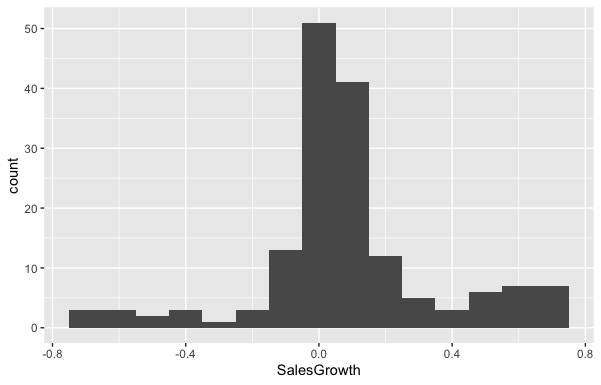
\includegraphics[width=7cm]{chinchilab-template/Pictures/Model1_hist_a.png}
    \end{subfigure}
    \begin{subfigure}
    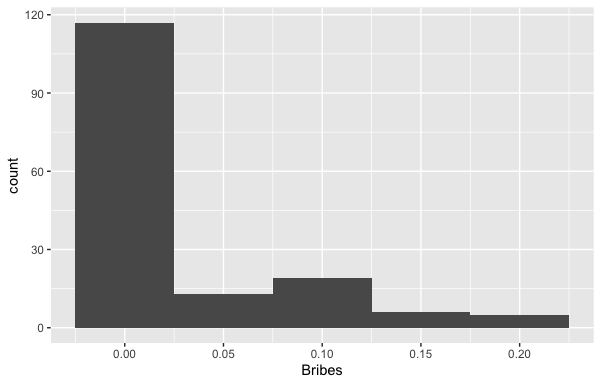
\includegraphics[width=7cm]{chinchilab-template/Pictures/Model1_hist_b.png}
    \end{subfigure}
    \begin{subfigure}
    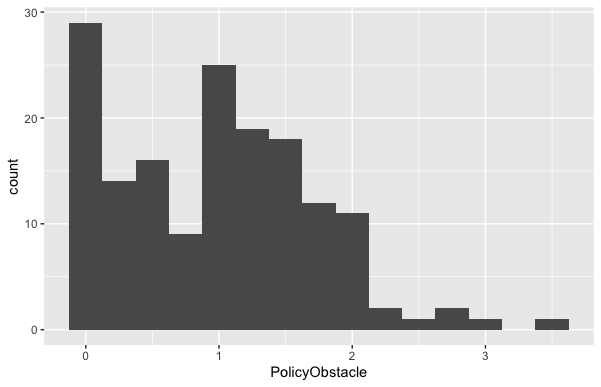
\includegraphics[width=7cm]{chinchilab-template/Pictures/Model1_hist_c.png}
    \end{subfigure}
    \begin{subfigure}
    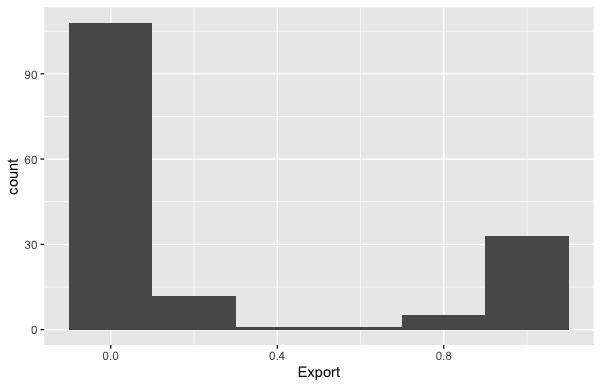
\includegraphics[width=7cm]{chinchilab-template/Pictures/Model1_hist_d.png}
    \end{subfigure}
    \caption*{Histogram of Continuous Variables}%
    \label{fig:example}}
\end{figure}

\begin{figure}[H]
    \centering
    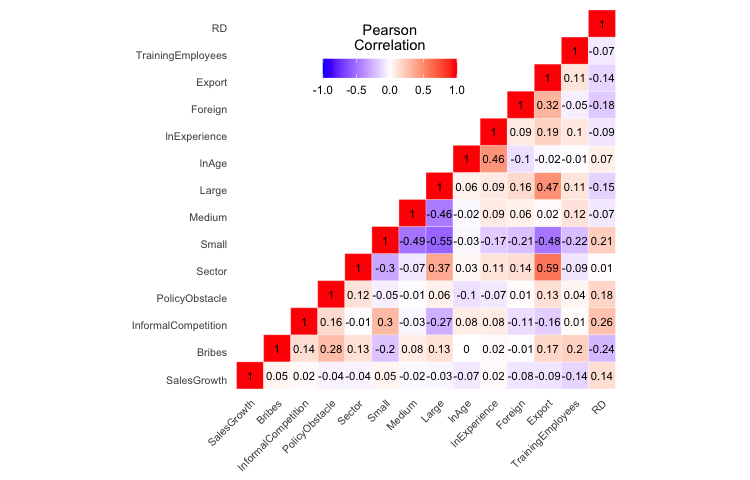
\includegraphics[scale=0.6]{chinchilab-template/Pictures/Model1_cor.png}
    \label{fig:my_label}
\end{figure}

\begin{table}[H]
\centering
\scalebox{0.7}{
\begin{tabular}{lllllll}
\hline
\multicolumn{7}{c}{Variance Inflation Factor (VIF)}                                          \\ \hline
Coefficients                & Baseline & Model 1 & Model 2a & Model 2b & Model 3a & Model 3b \\ \hline
Bribes                      &          & 1.12    & 1.24     & 6.31     & 1.21     & 3.62     \\
Policy Obstacle             &          &         & 1.21     & 1.57     &          &          \\
Bribes*Policy Obstacle      &          &         &          & 7.35     &          &          \\
Informal Competition        &          &         &          &          & 1.31     & 1.60     \\
Bribes*Informal Competition &          &         &          &          &          & 4.25    \\
Sector                      & 1.58     & 1.59    & 1.59     & 1.62     & 1.61     & 1.61     \\
Small                       & 2.02     & 2.02    & 2.02     & 2.07     & 2.24     & 2.25     \\
Medium                      & 1.50     & 1.50    & 1.50     & 1.53     & 1.54     & 1.54     \\
lnAge                       & 1.29     & 1.29    & 1.30     & 1.30     & 1.29     & 1.31     \\
lnExperience                & 1.34     & 1.34    & 1.34     & 1.34     & 1.34     & 1.38     \\
Foreign                     & 1.24     & 1.25    & 1.25     & 1.27     & 1.25     & 1.28     \\
Export                      & 2.06     & 2.06    & 2.11     & 2.13     & 2.07     & 2.07     \\
TrainingEmployees           & 1.12     & 1.15    & 1.15     & 1.16     & 1.16     & 1.16     \\
R\&D                        & 1.13     & 1.18    & 1.28     & 1.29     & 1.26     & 1.27 
\end{tabular}}
\end{table}

\begin{figure}[H]%
    \centering
    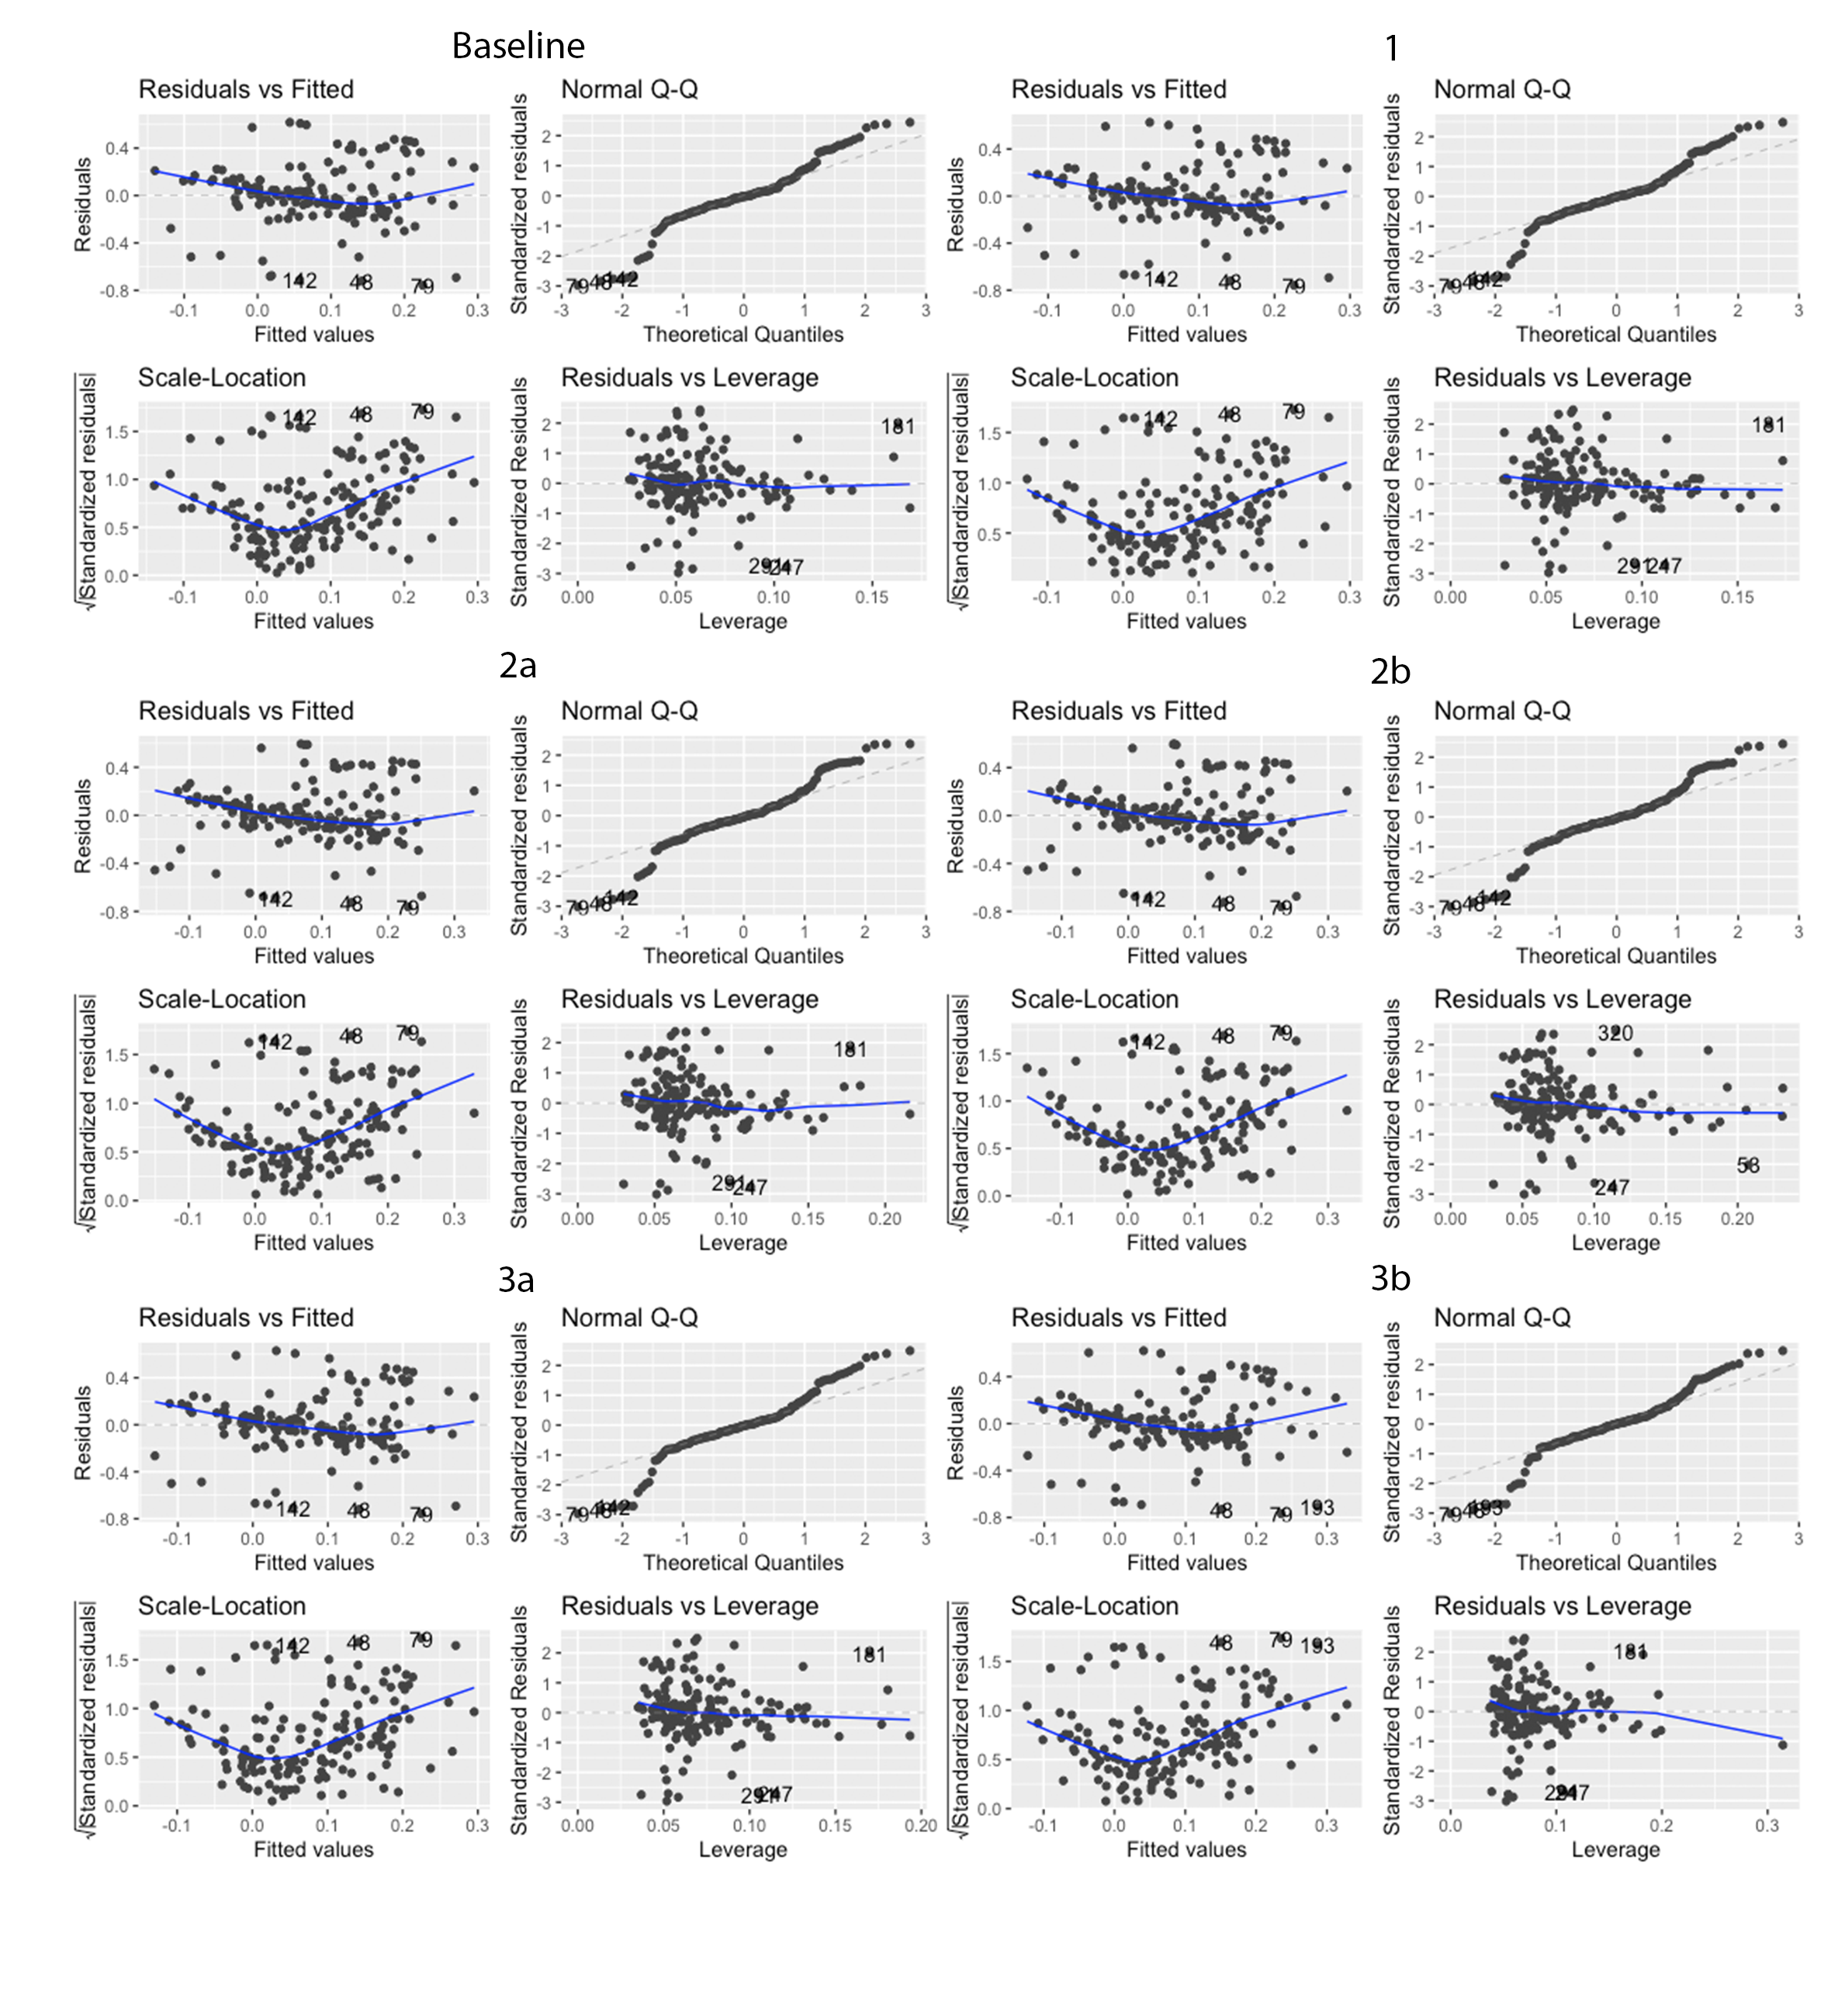
\includegraphics[scale=0.75]{chinchilab-template/Pictures/Model1_diag.png}
    \caption*{Diagnostic Plots}%
\end{figure}

\newpage

\textbf{\Large Model SBI}
\begin{table}[!htbp] \centering 
  \caption*{Summary Statistics} 
\begin{tabular}{@{\extracolsep{5pt}}lccccccc} 
\\[-1.8ex]\hline 
\hline \\[-1.8ex] 
Statistic & \multicolumn{1}{c}{N} & \multicolumn{1}{c}{Mean} & \multicolumn{1}{c}{St. Dev.} & \multicolumn{1}{c}{Min} & \multicolumn{1}{c}{Pctl(25)} & \multicolumn{1}{c}{Pctl(75)} & \multicolumn{1}{c}{Max} \\ 
\hline \\[-1.8ex] 
SalesGrowth & 244 & 0.073 & 0.250 & $-$0.666 & $-$0.016 & 0.108 & 0.667 \\ 
BribeIndex & 244 & 0.234 & 0.424 & 0 & 0 & 0 & 1 \\ 
InformalCompetition & 244 & 0.480 & 0.501 & 0 & 0 & 1 & 1 \\ 
PolicyObstacle & 244 & 1.075 & 0.784 & 0.000 & 0.500 & 1.750 & 3.500 \\ 
Sector & 244 & 0.430 & 0.496 & 0 & 0 & 1 & 1 \\ 
Small & 244 & 0.352 & 0.479 & 0 & 0 & 1 & 1 \\ 
Medium & 244 & 0.324 & 0.469 & 0 & 0 & 1 & 1 \\ 
Large & 244 & 0.324 & 0.469 & 0 & 0 & 1 & 1 \\ 
lnAge & 244 & 2.673 & 0.548 & 1.386 & 2.398 & 3.135 & 4.454 \\ 
lnExperience & 244 & 2.940 & 0.552 & 0.693 & 2.708 & 3.296 & 3.807 \\ 
Foreign & 244 & 0.088 & 0.276 & 0 & 0 & 0 & 1 \\ 
Export & 244 & 0.252 & 0.407 & 0 & 0 & 0.3 & 1 \\ 
TrainingEmployees & 244 & 0.439 & 0.497 & 0 & 0 & 1 & 1 \\ 
R\&D & 244 & 0.230 & 0.421 & 0 & 0 & 0 & 1 \\ 
\hline \\[-1.8ex] 
\end{tabular} 
\end{table} 

\begin{figure}[H]%
    \centering
    \begin{subfigure}
    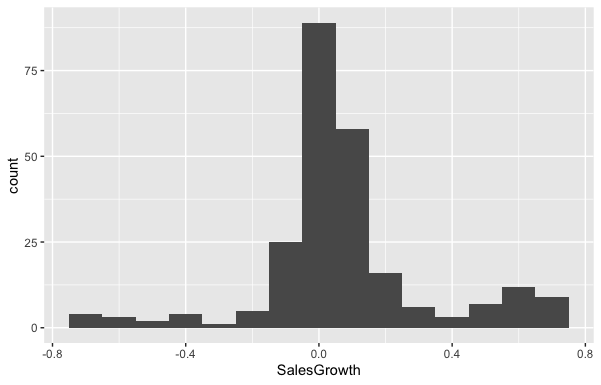
\includegraphics[width=7cm]{chinchilab-template/Pictures/Model1.2_hist_a.png}
    \end{subfigure}
    \begin{subfigure}
    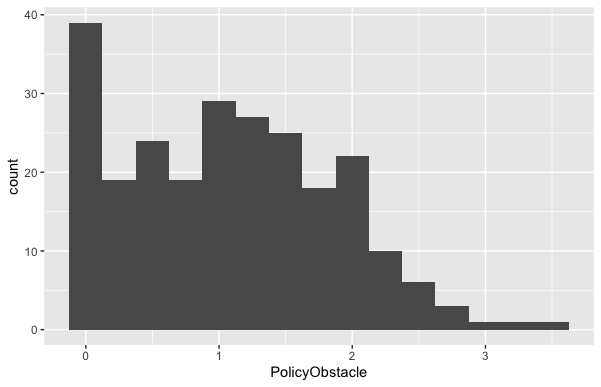
\includegraphics[width=7cm]{chinchilab-template/Pictures/Model1.2_hist_b.png}
    \end{subfigure}
    \begin{subfigure}
    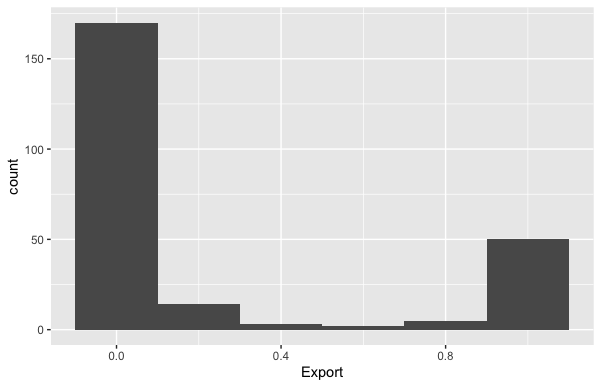
\includegraphics[width=7cm]{chinchilab-template/Pictures/Model1.2_hist_c.png}
    \end{subfigure}
    \begin{subfigure}
    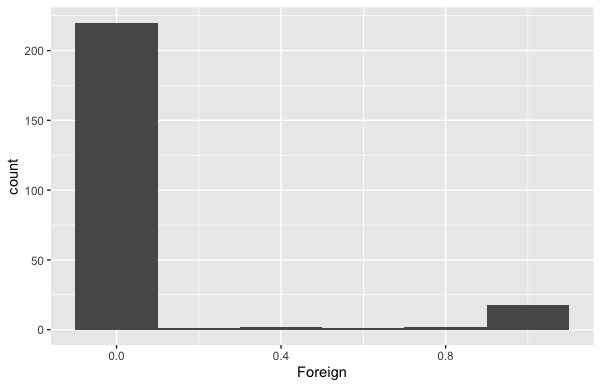
\includegraphics[width=7cm]{chinchilab-template/Pictures/Model1.2_hist_d.png}
    \end{subfigure}
    \caption*{Histogram of Continuous Variables}%
    \label{fig:example}%
\end{figure}

\begin{figure}[!t]
    \centering
    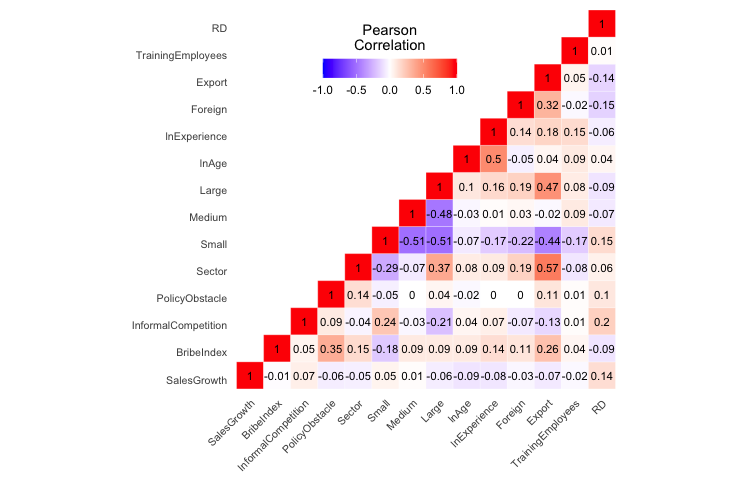
\includegraphics[scale=0.6]{chinchilab-template/Pictures/Model1.2_cor.png}
    \label{fig:my_label}
\end{figure}

\begin{table}[!h]
\centering
\scalebox{0.9}{%
\begin{tabular}{lllllll}
\hline
\multicolumn{7}{c}{Variance Inflation Factor (VIF)}                                          \\ \hline
Coefficients                & Baseline & Model 1 & Model 2a & Model 2b & Model 3a & Model 3b \\ \hline
BribeIndex                  &          & 1.10    & 1.23     & 5.87     & 1.11     & 2.23     \\
Policy Obstacle             &          &         & 1.17     & 1.45     &          &          \\
BribeIndex*Policy Obstacle      &          &         &          & 6.92     &          &          \\
Informal Competition        &          &         &          &          & 1.14     & 1.49     \\
BribeIndex*Informal Competition &          &         &          &          &          & 2.57    \\
Sector                      & 1.58     & 1.58    & 1.59     & 1.62     & 1.59     & 1.60     \\
Small                       & 2.02     & 2.02    & 2.03     & 2.04     & 2.13     & 2.13     \\
Medium                      & 1.58     & 1.59    & 1.59     & 1.62     & 1.61     & 1.61     \\
lnAge                       & 1.32     & 1.33    & 1.33     & 1.33     & 1.33     & 1.35     \\
lnExperience                & 1.35     & 1.35    & 1.35     & 1.36     & 1.36     & 1.38     \\
Foreign                     & 1.21     & 1.21    & 1.22     & 1.23     & 1.22     & 1.22     \\
Export                      & 2.05     & 2.11    & 2.12     & 2.20     & 2.12     & 2.12     \\
TrainingEmployees           & 1.09     & 1.09    & 1.09     & 1.09     & 1.09     & 1.09     \\
R\&D                        & 1.12     & 1.12    & 1.14     & 1.14     & 1.15     & 1.15     
\end{tabular}}
\end{table}

\begin{figure}[!tb]%
    \centering
    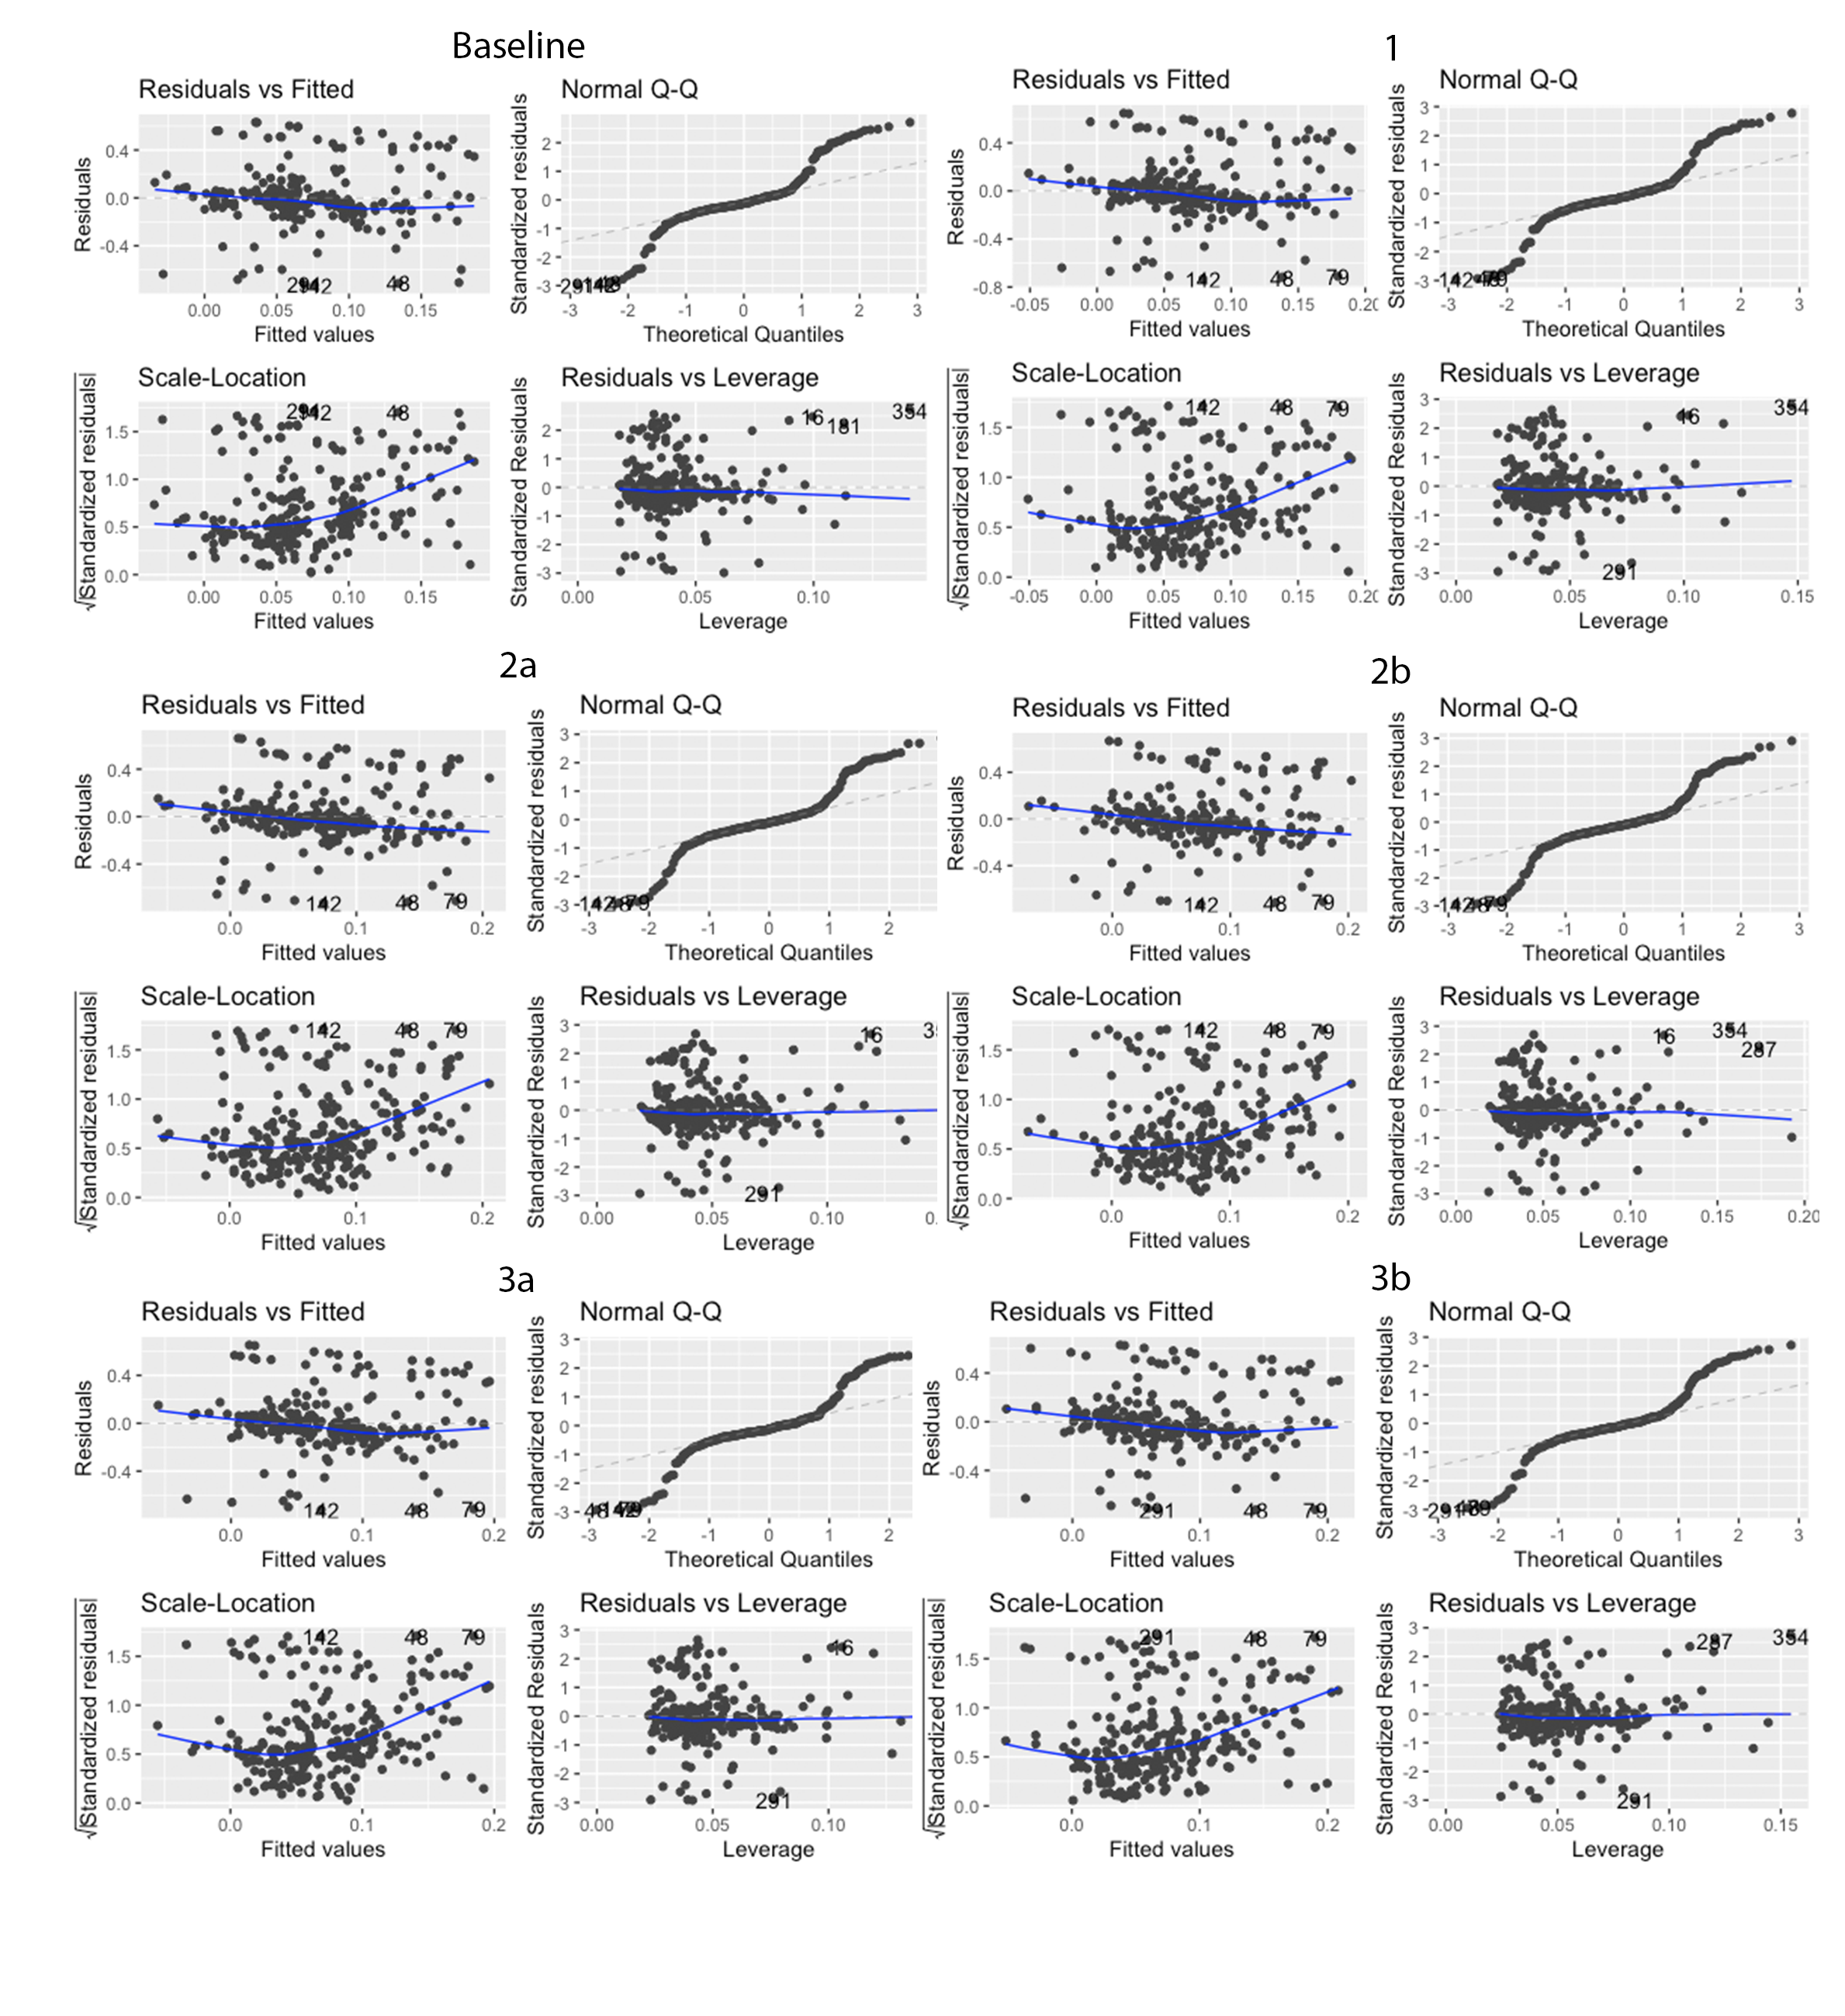
\includegraphics[scale=0.75]{chinchilab-template/Pictures/Model1.2_diag.png}
    \caption*{Diagnostic Plots}%
\end{figure}

\begin{landscape}
\thispagestyle{mylandscape}
\begin{table}[!htbp] \centering 
  \caption*{} 
  \begin{adjustbox}{width=\columnwidth,center}
\begin{tabular}{@{\extracolsep{5pt}}lD{.}{.}{-3} D{.}{.}{-3} D{.}{.}{-3} D{.}{.}{-3} D{.}{.}{-3} D{.}{.}{-3} } 
\\[-1.8ex]\hline 
\hline \\[-1.8ex] 
 & \multicolumn{6}{c}{\textit{Dependent variable:}} \\ 
\cline{2-7} 
\\[-1.8ex] & \multicolumn{6}{c}{SalesGrowth} \\ 
\\[-1.8ex] & \multicolumn{1}{c}{(1)} & \multicolumn{1}{c}{(2)} & \multicolumn{1}{c}{(3)} & \multicolumn{1}{c}{(4)} & \multicolumn{1}{c}{(5)} & \multicolumn{1}{c}{(6)}\\ 
\hline \\[-1.8ex] 
  BribeIndex &  & -0.025 & -0.005 & 0.029 & -0.027 & 0.013 \\ 
  &  & (0.040) & (0.042) & (0.092) & (0.040) & (0.057) \\ 
  PolicyObstacle &  &  & -0.032 & -0.028 &  &  \\ 
  &  &  & (0.022) & (0.025) &  &  \\ 
  BribeIndex $\times$ PolicyObstacle &  &  &  & -0.024 &  &  \\ 
  &  &  &  & (0.058) &  &  \\ 
  InformalCompetition &  &  &  &  & 0.021 & 0.040 \\ 
  &  &  &  &  & (0.034) & (0.039) \\ 
  BribeIndex $\times$ InformalCompetition &  &  &  &  &  & -0.080 \\ 
  &  &  &  &  &  & (0.079) \\ 
 Sector & -0.042 & -0.041 & -0.038 & -0.040 & -0.043 & -0.046 \\ 
  & (0.041) & (0.041) & (0.041) & (0.041) & (0.041) & (0.041) \\ 
  Small & 0.039 & 0.039 & 0.040 & 0.039 & 0.032 & 0.031 \\ 
  & (0.048) & (0.048) & (0.048) & (0.048) & (0.049) & (0.049) \\ 
  Medium & 0.045 & 0.048 & 0.048 & 0.046 & 0.045 & 0.047 \\ 
  & (0.043) & (0.043) & (0.043) & (0.044) & (0.044) & (0.044) \\ 
  lnAge & 0.0002 & 0.002 & -0.001 & -0.002 & 0.002 & -0.003 \\ 
  & (0.034) & (0.034) & (0.034) & (0.034) & (0.034) & (0.034) \\ 
  lnExperience & 0.025 & 0.025 & 0.024 & 0.022 & 0.023 & 0.028 \\ 
  & (0.034) & (0.034) & (0.034) & (0.034) & (0.034) & (0.034) \\ 
  Foreign & 0.043 & 0.043 & 0.040 & 0.037 & 0.043 & 0.045 \\ 
  & (0.064) & (0.064) & (0.064) & (0.065) & (0.064) & (0.064) \\ 
  Export & 0.040 & 0.046 & 0.050 & 0.055 & 0.048 & 0.046 \\ 
  & (0.057) & (0.057) & (0.057) & (0.059) & (0.058) & (0.058) \\ 
  TrainingEmployees & -0.042 & -0.042 & -0.041 & -0.041 & -0.042 & -0.041 \\ 
  & (0.034) & (0.034) & (0.034) & (0.034) & (0.034) & (0.034) \\ 
  R\&D & \cellcolor{yellow}0.081^{**} & \cellcolor{yellow}0.080^{**} & \cellcolor{yellow}0.087^{**} & \cellcolor{yellow}0.087^{**} & \cellcolor{yellow}0.076^{*} & \cellcolor{yellow}0.073^{*} \\ 
  & (0.040) & (0.040) & (0.041) & (0.041) & (0.041) & (0.041) \\ 
  Constant & -0.025 & -0.026 & 0.010 & 0.013 & -0.025 & -0.033 \\ 
  & (0.110) & (0.110) & (0.112) & (0.113) & (0.110) & (0.110) \\ 
 \hline \\[-1.8ex] 
Observations & \multicolumn{1}{c}{244} & \multicolumn{1}{c}{244} & \multicolumn{1}{c}{244} & \multicolumn{1}{c}{244} & \multicolumn{1}{c}{244} & \multicolumn{1}{c}{244} \\ 
R$^{2}$ & \multicolumn{1}{c}{0.033} & \multicolumn{1}{c}{0.034} & \multicolumn{1}{c}{0.043} & \multicolumn{1}{c}{0.044} & \multicolumn{1}{c}{0.036} & \multicolumn{1}{c}{0.040} \\ 
Adjusted R$^{2}$ & \multicolumn{1}{c}{-0.005} & \multicolumn{1}{c}{-0.007} & \multicolumn{1}{c}{-0.002} & \multicolumn{1}{c}{-0.006} & \multicolumn{1}{c}{-0.010} & \multicolumn{1}{c}{-0.010} \\ 
Residual Std. Error & \multicolumn{1}{c}{0.251 (df = 234)} & \multicolumn{1}{c}{0.251 (df = 233)} & \multicolumn{1}{c}{0.250 (df = 232)} & \multicolumn{1}{c}{0.251 (df = 231)} & \multicolumn{1}{c}{0.251 (df = 232)} & \multicolumn{1}{c}{0.251 (df = 231)} \\ 
F Statistic & \multicolumn{1}{c}{0.874 (df = 9; 234)} & \multicolumn{1}{c}{0.823 (df = 10; 233)} & \multicolumn{1}{c}{0.946 (df = 11; 232)} & \multicolumn{1}{c}{0.878 (df = 12; 231)} & \multicolumn{1}{c}{0.779 (df = 11; 232)} & \multicolumn{1}{c}{0.800 (df = 12; 231)} \\ 
\hline 
\hline \\[-1.8ex] 
\textit{Note:}  & \multicolumn{6}{r}{$^{*}$p$<$0.1; $^{**}$p$<$0.05; $^{***}$p$<$0.01} \\ 
\end{tabular} 
\end{adjustbox}
\end{table} 
\end{landscape}

\textbf{\Large Model SIB}

\begin{table}[!h] \centering 
  \caption*{Summary Statistics} 
\begin{tabular}{@{\extracolsep{5pt}}lccccccc} 
\\[-1.8ex]\hline 
\hline \\[-1.8ex] 
Statistic & \multicolumn{1}{c}{N} & \multicolumn{1}{c}{Mean} & \multicolumn{1}{c}{St. Dev.} & \multicolumn{1}{c}{Min} & \multicolumn{1}{c}{Pctl(25)} & \multicolumn{1}{c}{Pctl(75)} & \multicolumn{1}{c}{Max} \\ 
\hline \\[-1.8ex] 
SalesGrowth & 227 & 0.078 & 0.251 & $-$0.660 & $-$0.012 & 0.109 & 0.667 \\ 
Inspection.Bribe & 227 & 0.322 & 0.468 & 0 & 0 & 1 & 1 \\ 
InformalCompetition & 227 & 0.476 & 0.501 & 0 & 0 & 1 & 1 \\ 
PolicyObstacle & 227 & 1.080 & 0.783 & 0.000 & 0.500 & 1.750 & 3.500 \\ 
Sector & 227 & 0.432 & 0.496 & 0 & 0 & 1 & 1 \\ 
Small & 227 & 0.357 & 0.480 & 0 & 0 & 1 & 1 \\ 
Medium & 227 & 0.317 & 0.466 & 0 & 0 & 1 & 1 \\ 
Large & 227 & 0.326 & 0.470 & 0 & 0 & 1 & 1 \\ 
lnAge & 227 & 2.678 & 0.544 & 1.386 & 2.398 & 3.135 & 4.454 \\ 
lnExperience & 227 & 2.946 & 0.538 & 0.693 & 2.708 & 3.258 & 3.807 \\ 
Foreign & 227 & 0.077 & 0.262 & 0 & 0 & 0 & 1 \\ 
Export & 227 & 0.248 & 0.405 & 0 & 0 & 0.3 & 1 \\ 
TrainingEmployees & 227 & 0.458 & 0.499 & 0 & 0 & 1 & 1 \\ 
R\&D & 227 & 0.247 & 0.432 & 0 & 0 & 0 & 1 \\ 
\hline \\[-1.8ex] 
\end{tabular} 
\end{table} 

\begin{figure}[H]%
    \centering
    \begin{subfigure}
    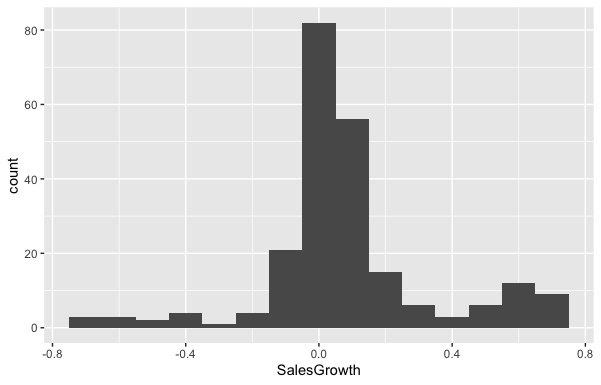
\includegraphics[width=7cm]{chinchilab-template/Pictures/Model1.3_hist_a.png}
    \end{subfigure}
    \begin{subfigure}
    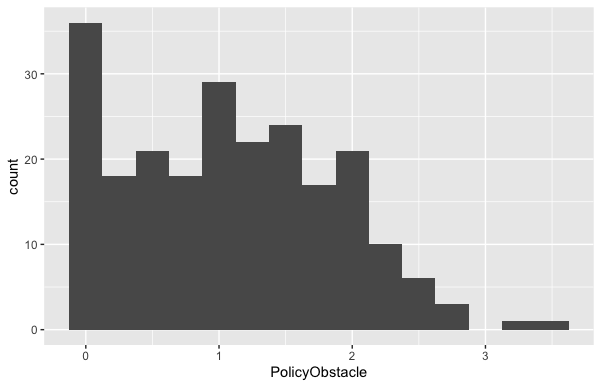
\includegraphics[width=7cm]{chinchilab-template/Pictures/Model1.3_hist_b.png}
    \end{subfigure}
    \begin{subfigure}
    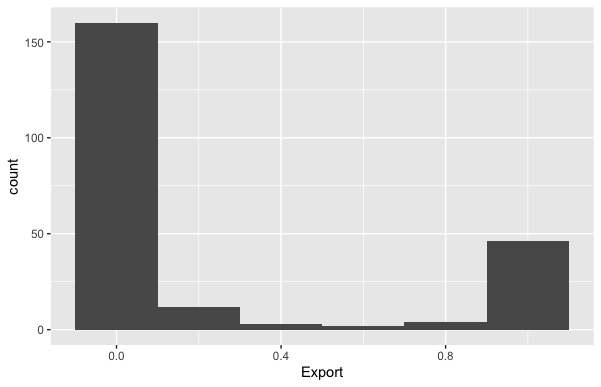
\includegraphics[width=7cm]{chinchilab-template/Pictures/Model1.3_hist_c.png}
    \end{subfigure}
    \begin{subfigure}
    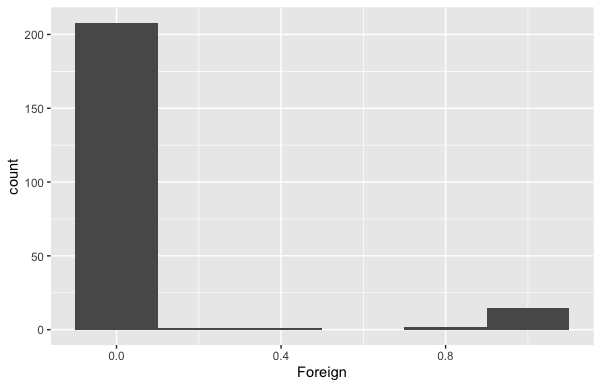
\includegraphics[width=7cm]{chinchilab-template/Pictures/Model1.3_hist_d.png}
    \end{subfigure}
    \caption*{Histogram of Continuous Variables}%
    \label{fig:example}%
\end{figure}

\begin{figure}[H]
    \centering
    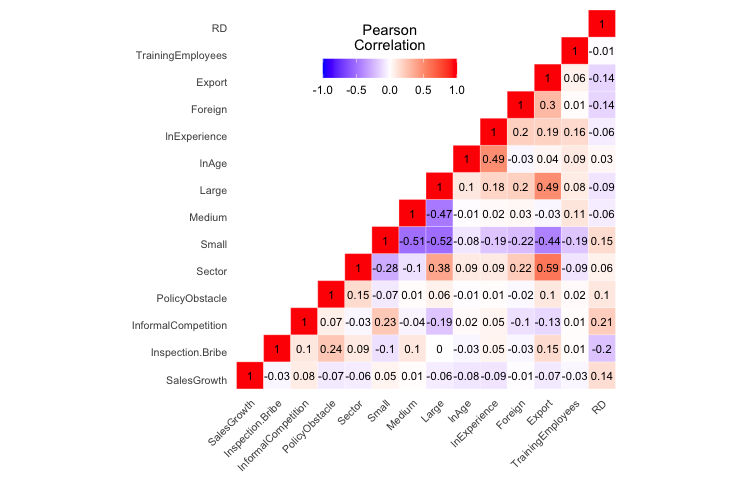
\includegraphics[scale=0.6]{chinchilab-template/Pictures/Model1.3_cor.png}
    \label{fig:my_label}
\end{figure}

\begin{table}[!h]
\centering
\scalebox{0.9}{%
\begin{tabular}{lllllll}
\hline
\multicolumn{7}{c}{Variance Inflation Factor (VIF)}                                          \\ \hline
Coefficients                & Baseline & Model 1 & Model 2a & Model 2b & Model 3a & Model 3b \\ \hline
Inspection.Bribe            &          & 1.08    & 1.14     & 3.92     & 1.10     & 2.18     \\
Policy Obstacle             &          &         & 1.10     & 1.61     &          &          \\
Inspection.Bribe*Policy Obstacle      &          &         &          & 4.96     &          &          \\
Informal Competition        &          &         &          &          & 1.15     & 1.71     \\
Inspection.Bribe*Informal Competition &          &         &          &          &          & 2.91    \\
Sector                      & 1.62     & 1.64    & 1.64     & 1.67     & 1.64     & 1.64     \\
Small                       & 2.06     & 2.06    & 2.06     & 2.06     & 2.14     & 2.15     \\
Medium                      & 1.62     & 1.63    & 1.63     & 1.64     & 1.64     & 1.64     \\
lnAge                       & 1.31     & 1.32    & 1.32     & 1.33     & 1.32     & 1.32     \\
lnExperience                & 1.34     & 1.35    & 1.35     & 1.36     & 1.36     & 1.37     \\
Foreign                     & 1.22     & 1.23    & 1.23     & 1.24     & 1.23     & 1.23     \\
Export                      & 2.10     & 2.10    & 2.11     & 2.16     & 2.11     & 2.11     \\
TrainingEmployees           & 1.09     & 1.09    & 1.09     & 1.12     & 1.09     & 1.14     \\
R\&D                        & 1.12     & 1.17    & 1.19     & 1.20     & 1.21     & 1.24     
\end{tabular}}
\end{table}

\begin{figure}[!t]%
    \centering
    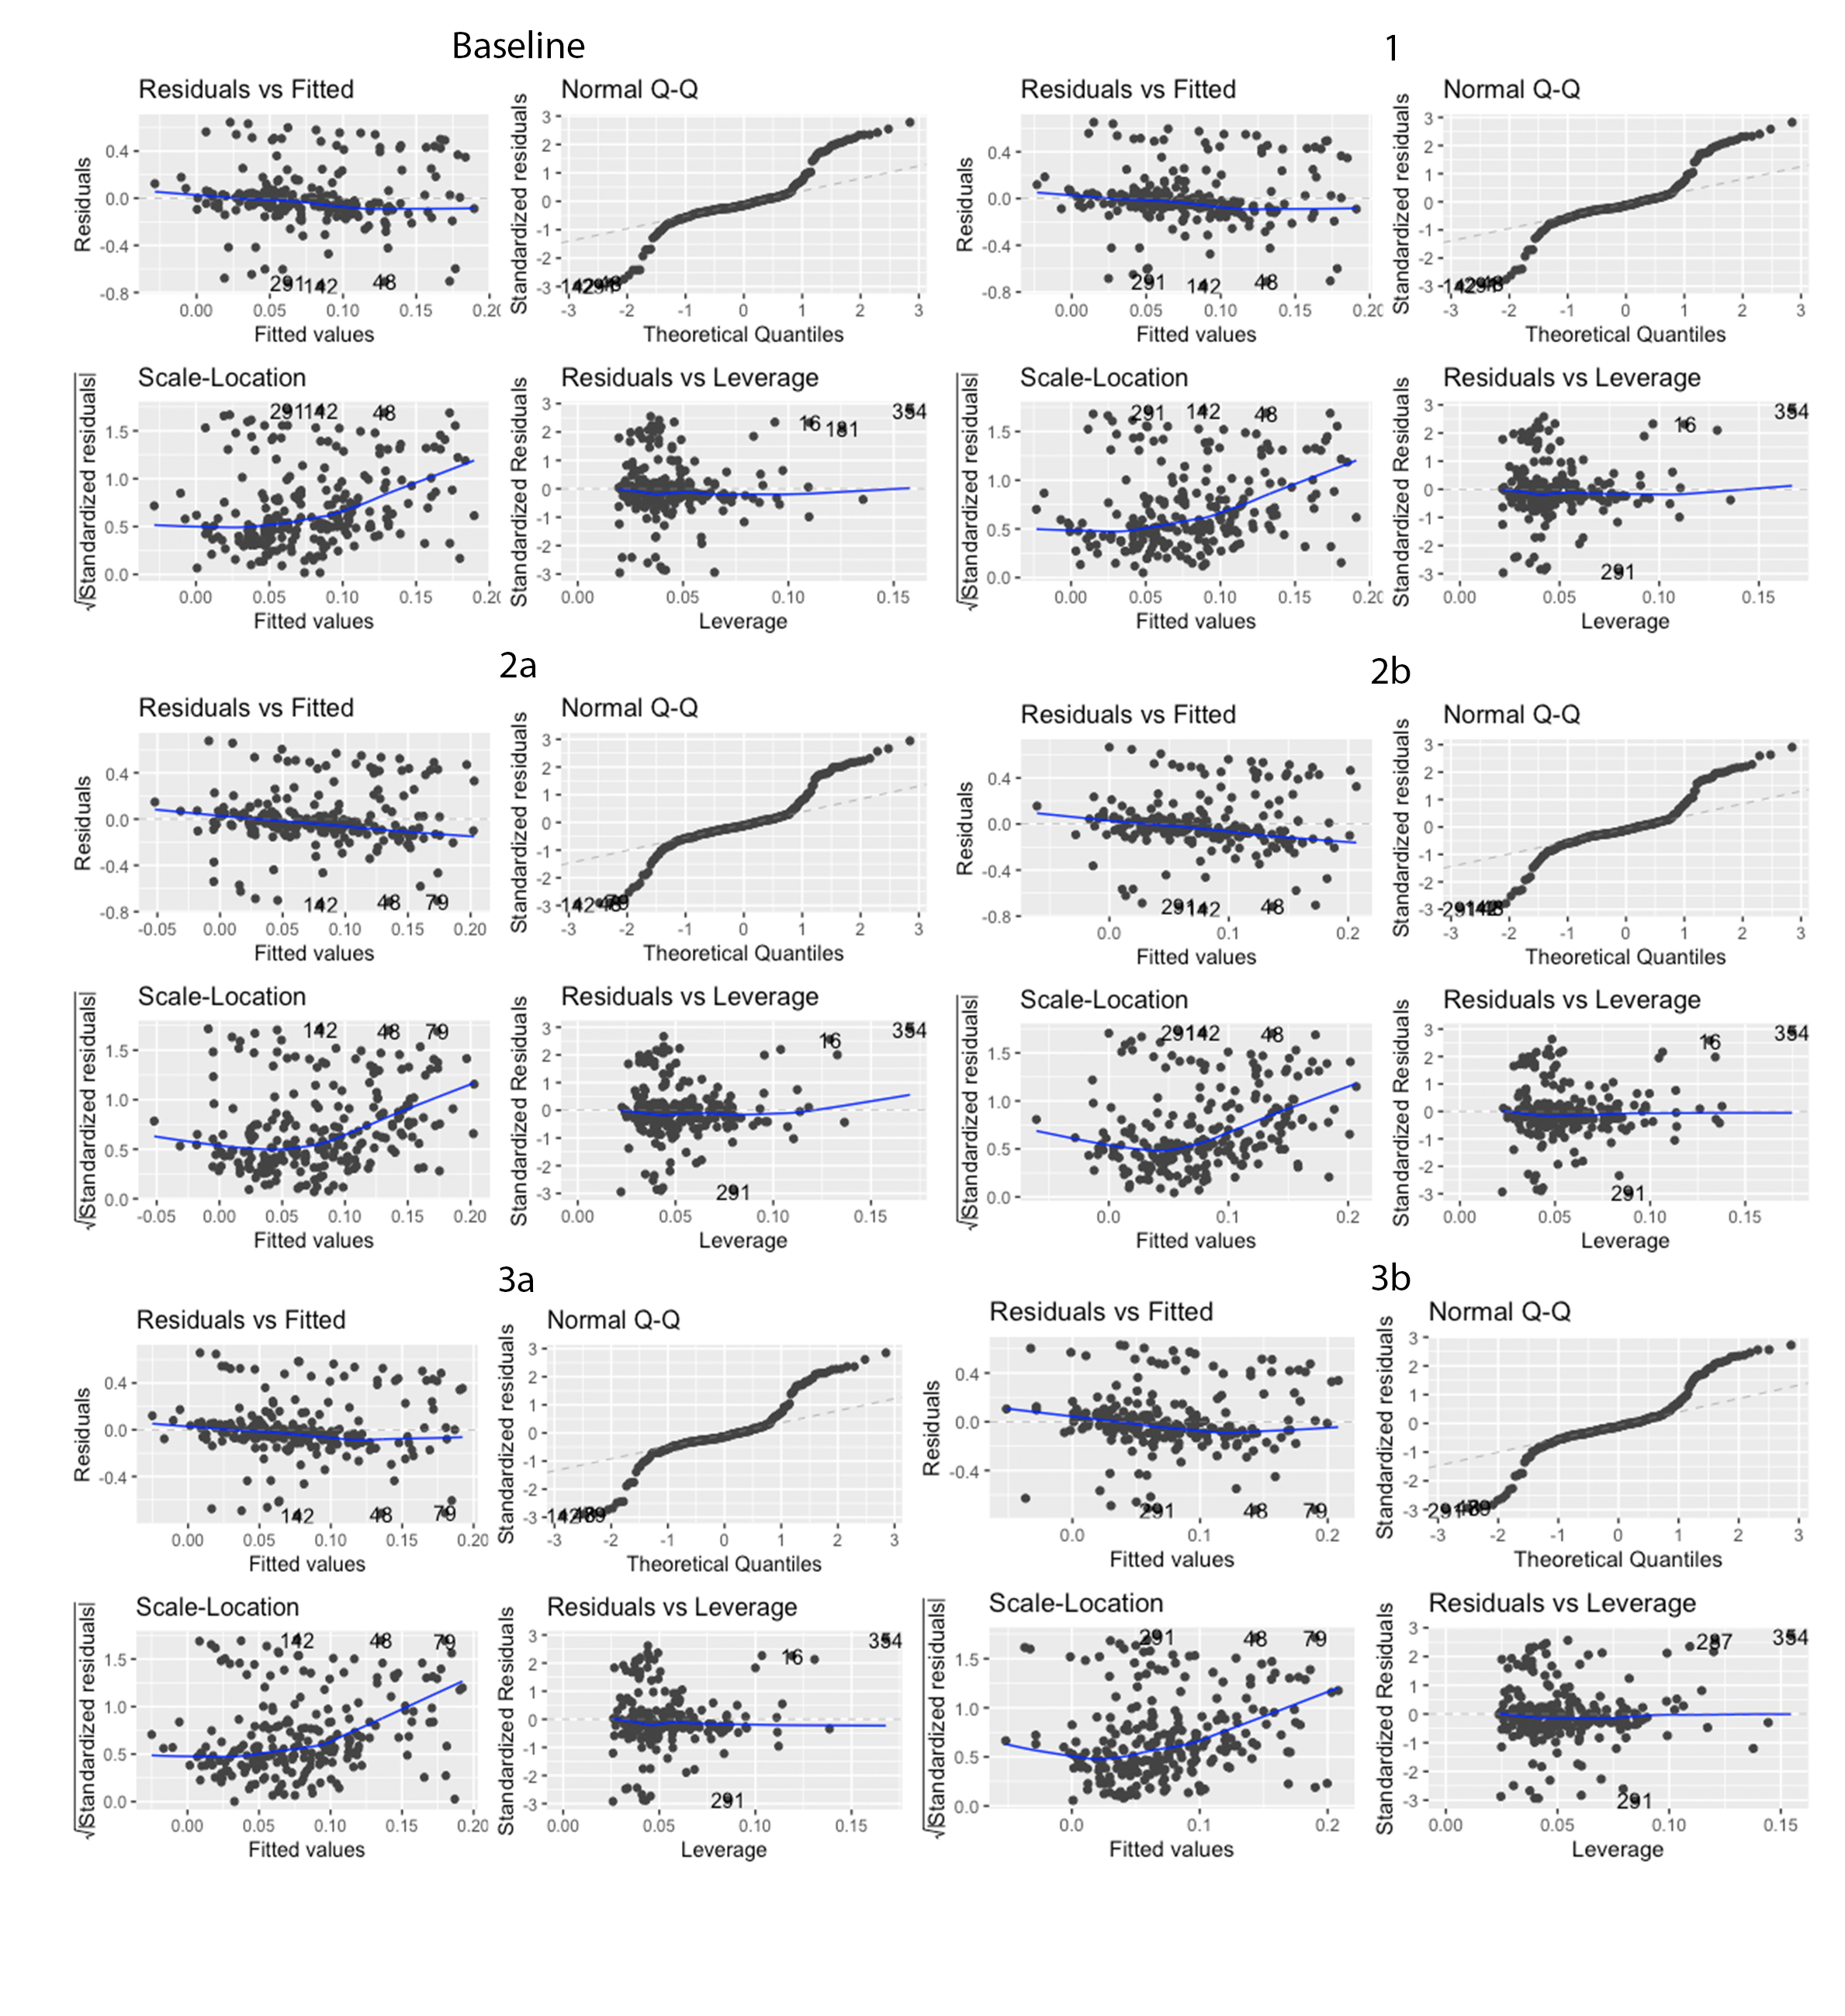
\includegraphics[scale=0.75]{chinchilab-template/Pictures/Model1.3_diag.png}
    \caption*{Diagnostic Plots}%
\end{figure}

\begin{landscape}
\thispagestyle{mylandscape}
\begin{table}[!h] \centering 
  \caption*{} 
  \begin{adjustbox}{width=\columnwidth,center}
\begin{tabular}{@{\extracolsep{5pt}}lD{.}{.}{-3} D{.}{.}{-3} D{.}{.}{-3} D{.}{.}{-3} D{.}{.}{-3} D{.}{.}{-3} } 
\\[-1.8ex]\hline 
\hline \\[-1.8ex] 
 & \multicolumn{6}{c}{\textit{Dependent variable:}} \\ 
\cline{2-7} 
\\[-1.8ex] & \multicolumn{6}{c}{SalesGrowth} \\ 
\\[-1.8ex] & \multicolumn{1}{c}{(1)} & \multicolumn{1}{c}{(2)} & \multicolumn{1}{c}{(3)} & \multicolumn{1}{c}{(4)} & \multicolumn{1}{c}{(5)} & \multicolumn{1}{c}{(6)}\\ 
\hline \\[-1.8ex] 
  Inspection.Bribe &  & -0.013 & 0.002 & -0.029 & -0.017 & 0.004 \\ 
  &  & (0.037) & (0.038) & (0.071) & (0.038) & (0.053) \\ 
  PolicyObstacle &  &  & -0.037 & -0.045 &  &  \\ 
  &  &  & (0.022) & (0.027) &  &  \\ 
  Inspection.Bribe $\times$ PolicyObstacle &  &  &  & 0.025 &  &  \\ 
  &  &  &  & (0.050) &  &  \\ 
  InformalCompetition &  &  &  &  & 0.026 & 0.040 \\ 
  &  &  &  &  & (0.036) & (0.044) \\ 
  Inspection.Bribe $\times$ InformalCompetition &  &  &  &  &  & -0.043 \\ 
  &  &  &  &  &  & (0.075) \\ 
 Sector & -0.044 & -0.043 & -0.038 & -0.036 & -0.044 & -0.045 \\ 
  & (0.043) & (0.043) & (0.043) & (0.044) & (0.044) & (0.044) \\ 
  Small & 0.026 & 0.026 & 0.025 & 0.025 & 0.019 & 0.020 \\ 
  & (0.050) & (0.050) & (0.050) & (0.050) & (0.051) & (0.052) \\ 
  Medium & 0.030 & 0.031 & 0.032 & 0.030 & 0.029 & 0.030 \\ 
  & (0.046) & (0.046) & (0.046) & (0.046) & (0.046) & (0.046) \\ 
  lnAge & -0.003 & -0.004 & -0.005 & -0.006 & -0.004 & -0.006 \\ 
  & (0.035) & (0.036) & (0.035) & (0.036) & (0.036) & (0.036) \\ 
  lnExperience & 0.023 & 0.024 & 0.022 & 0.023 & 0.021 & 0.022 \\ 
  & (0.036) & (0.036) & (0.036) & (0.036) & (0.037) & (0.037) \\ 
  Foreign & 0.075 & 0.073 & 0.069 & 0.071 & 0.073 & 0.073 \\ 
  & (0.071) & (0.071) & (0.071) & (0.071) & (0.071) & (0.071) \\ 
  Export & 0.021 & 0.021 & 0.028 & 0.024 & 0.023 & 0.023 \\ 
  & (0.060) & (0.060) & (0.060) & (0.061) & (0.060) & (0.061) \\ 
  TrainingEmployees & -0.041 & -0.041 & -0.040 & -0.037 & -0.042 & -0.038 \\ 
  & (0.035) & (0.035) & (0.035) & (0.036) & (0.035) & (0.036) \\ 
  R\&D & \cellcolor{yellow}0.073^{*} & \cellcolor{yellow}0.070^{*} & \cellcolor{yellow}0.080^{*} & \cellcolor{yellow}0.081^{*} & 0.064 & 0.060 \\ 
  & (0.041) & (0.042) & (0.042) & (0.043) & (0.043) & (0.044) \\ 
  Constant & 0.010 & 0.013 & 0.049 & 0.055 & 0.016 & 0.008 \\ 
  & (0.118) & (0.118) & (0.120) & (0.121) & (0.119) & (0.120) \\ 
 \hline \\[-1.8ex] 
Observations & \multicolumn{1}{c}{227} & \multicolumn{1}{c}{227} & \multicolumn{1}{c}{227} & \multicolumn{1}{c}{227} & \multicolumn{1}{c}{227} & \multicolumn{1}{c}{227} \\ 
R$^{2}$ & \multicolumn{1}{c}{0.030} & \multicolumn{1}{c}{0.031} & \multicolumn{1}{c}{0.043} & \multicolumn{1}{c}{0.044} & \multicolumn{1}{c}{0.033} & \multicolumn{1}{c}{0.035} \\ 
Adjusted R$^{2}$ & \multicolumn{1}{c}{-0.010} & \multicolumn{1}{c}{-0.014} & \multicolumn{1}{c}{-0.006} & \multicolumn{1}{c}{-0.009} & \multicolumn{1}{c}{-0.016} & \multicolumn{1}{c}{-0.019} \\ 
Residual Std. Error & \multicolumn{1}{c}{0.252 (df = 217)} & \multicolumn{1}{c}{0.253 (df = 216)} & \multicolumn{1}{c}{0.252 (df = 215)} & \multicolumn{1}{c}{0.252 (df = 214)} & \multicolumn{1}{c}{0.253 (df = 215)} & \multicolumn{1}{c}{0.254 (df = 214)} \\ 
F Statistic & \multicolumn{1}{c}{0.754 (df = 9; 217)} & \multicolumn{1}{c}{0.688 (df = 10; 216)} & \multicolumn{1}{c}{0.877 (df = 11; 215)} & \multicolumn{1}{c}{0.823 (df = 12; 214)} & \multicolumn{1}{c}{0.671 (df = 11; 215)} & \multicolumn{1}{c}{0.641 (df = 12; 214)} \\ 
\hline 
\hline \\[-1.8ex] 
\textit{Note:}  & \multicolumn{6}{r}{$^{*}$p$<$0.1; $^{**}$p$<$0.05; $^{***}$p$<$0.01} \\ 
\end{tabular} 
\end{adjustbox}
\end{table} 
\end{landscape}

\textbf{\Large Model EB}

\begin{table}[!ht] \centering 
  \caption*{Summary Statistics} 
  \scalebox{0.8}{%
\begin{tabular}{@{\extracolsep{5pt}}lccccccc} 
\\[-1.8ex]\hline 
\hline \\[-1.8ex] 
Statistic & \multicolumn{1}{c}{N} & \multicolumn{1}{c}{Mean} & \multicolumn{1}{c}{St. Dev.} & \multicolumn{1}{c}{Min} & \multicolumn{1}{c}{Pctl(25)} & \multicolumn{1}{c}{Pctl(75)} & \multicolumn{1}{c}{Max} \\ 
\hline \\[-1.8ex] 
EmploymentGrowth & 163 & 0.032 & 0.113 & $-$0.666 & 0.000 & 0.075 & 0.400 \\ 
Bribes & 163 & 0.030 & 0.054 & 0.000 & 0.000 & 0.050 & 0.200 \\ 
InformalCompetition & 163 & 0.552 & 0.499 & 0 & 0 & 1 & 1 \\ 
PolicyObstacle & 163 & 0.997 & 0.740 & 0 & 0.2 & 1.5 & 4 \\ 
Sector & 163 & 0.436 & 0.497 & 0 & 0 & 1 & 1 \\ 
Small & 163 & 0.380 & 0.487 & 0 & 0 & 1 & 1 \\ 
Medium & 163 & 0.294 & 0.457 & 0 & 0 & 1 & 1 \\ 
Large & 163 & 0.325 & 0.470 & 0 & 0 & 1 & 1 \\ 
lnAge & 163 & 2.620 & 0.553 & 1.386 & 2.250 & 3.091 & 3.367 \\ 
lnExperience & 163 & 2.932 & 0.540 & 1.099 & 2.674 & 3.277 & 3.807 \\ 
Foreign & 163 & 0.083 & 0.266 & 0 & 0 & 0 & 1 \\ 
Export & 163 & 0.265 & 0.415 & 0 & 0 & 0.5 & 1 \\ 
TrainingEmployees & 163 & 0.350 & 0.478 & 0 & 0 & 1 & 1 \\ 
R\&D & 163 & 0.239 & 0.428 & 0 & 0 & 0 & 1 \\ 
\hline \\[-1.8ex] 
\end{tabular}}
\end{table} 

\begin{figure}[scale=0.8]%
    \centering
    \begin{subfigure}
    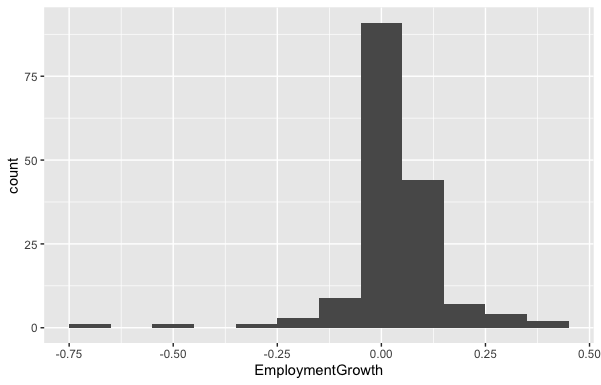
\includegraphics[width=7cm]{chinchilab-template/Pictures/Model2_hist_a.png}
    \end{subfigure}
    \begin{subfigure}
    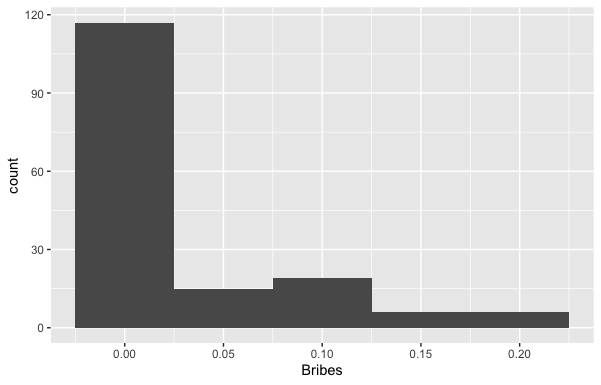
\includegraphics[width=7cm]{chinchilab-template/Pictures/Model2_hist_b.png}
    \end{subfigure}
    \begin{subfigure}
    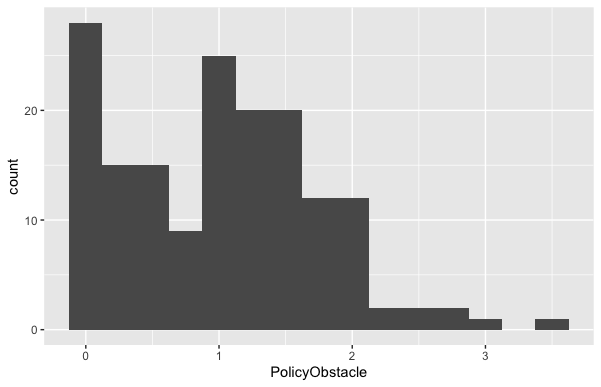
\includegraphics[width=7cm]{chinchilab-template/Pictures/Model2_hist_c.png}
    \end{subfigure}
    \begin{subfigure}
    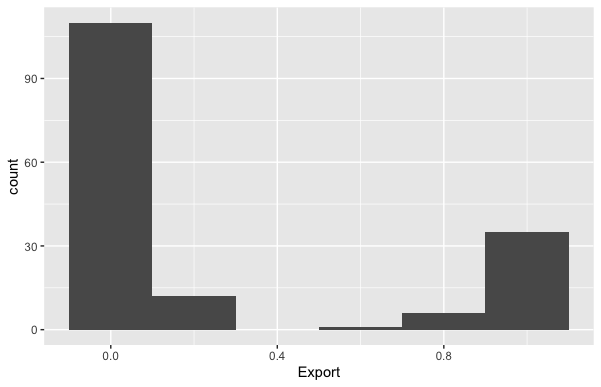
\includegraphics[width=7cm]{chinchilab-template/Pictures/Model2_hist_d.png}
    \end{subfigure}
    \begin{subfigure}
    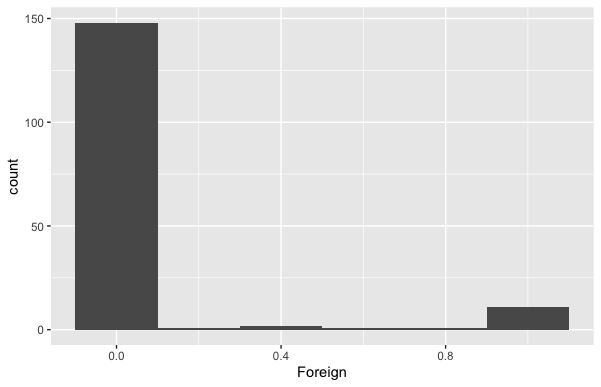
\includegraphics[width=7cm]{chinchilab-template/Pictures/Model2_hist_e.png}
    \end{subfigure}
    \caption*{Histogram of Continuous Variables}%
    \label{fig:example}%
\end{figure}

\begin{figure}[H]
    \centering
    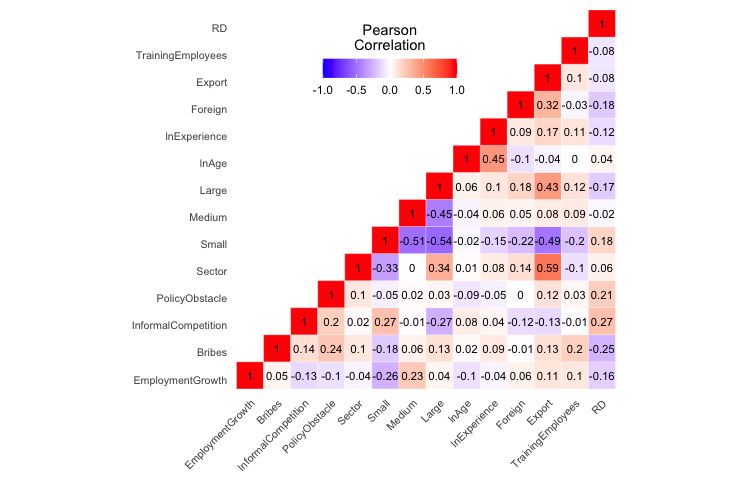
\includegraphics[scale=0.6]{chinchilab-template/Pictures/Model2_cor.png}
    \label{fig:my_label}
\end{figure}

\begin{table}[]
\centering
\scalebox{0.9}{%
\begin{tabular}{lllllll}
\hline
\multicolumn{7}{c}{Variance Inflation Factor (VIF)}                                          \\ \hline
Coefficients                & Baseline & Model 1 & Model 2a & Model 2b & Model 3a & Model 3b \\ \hline
Bribes                      &          & 1.12    & 1.23     & 6.28     & 1.19     & 2.98     \\
Policy Obstacle             &          &         & 1.20     & 1.59     &          &          \\
Bribes*Policy Obstacle      &          &         &          & 7.36     &          &          \\
Informal Competition        &          &         &          &          & 1.29     & 1.64     \\
Bribes*Informal Competition &          &         &          &          &          & 3.64  \\
Sector                      & 1.60     & 1.60    & 1.60     & 1.63     & 1.63     & 1.63     \\
Small                       & 2.06     & 2.06    & 2.06     & 2.11     & 2.26     & 2.26     \\
Medium                      & 1.49     & 1.49    & 1.49     & 1.52     & 1.53     & 1.53     \\
lnAge                       & 1.29     & 1.29    & 1.30     & 1.30     & 1.30     & 1.30     \\
lnExperience                & 1.33     & 1.33    & 1.33     & 1.33     & 1.33     & 1.35     \\
Foreign                     & 1.23     & 1.24    & 1.25     & 1.26     & 1.24     & 1.27     \\
Export                      & 1.99     & 1.99    & 2.04     & 2.06     & 2.00     & 2.00     \\
TrainingEmployees           & 1.11     & 1.14    & 1.14     & 1.15     & 1.14     & 1.16     \\
R\&D                        & 1.13     & 1.19    & 1.30     & 1.30     & 1.27     & 1.29     
\end{tabular}}
\end{table}

\begin{figure}[!t]%
    \centering
    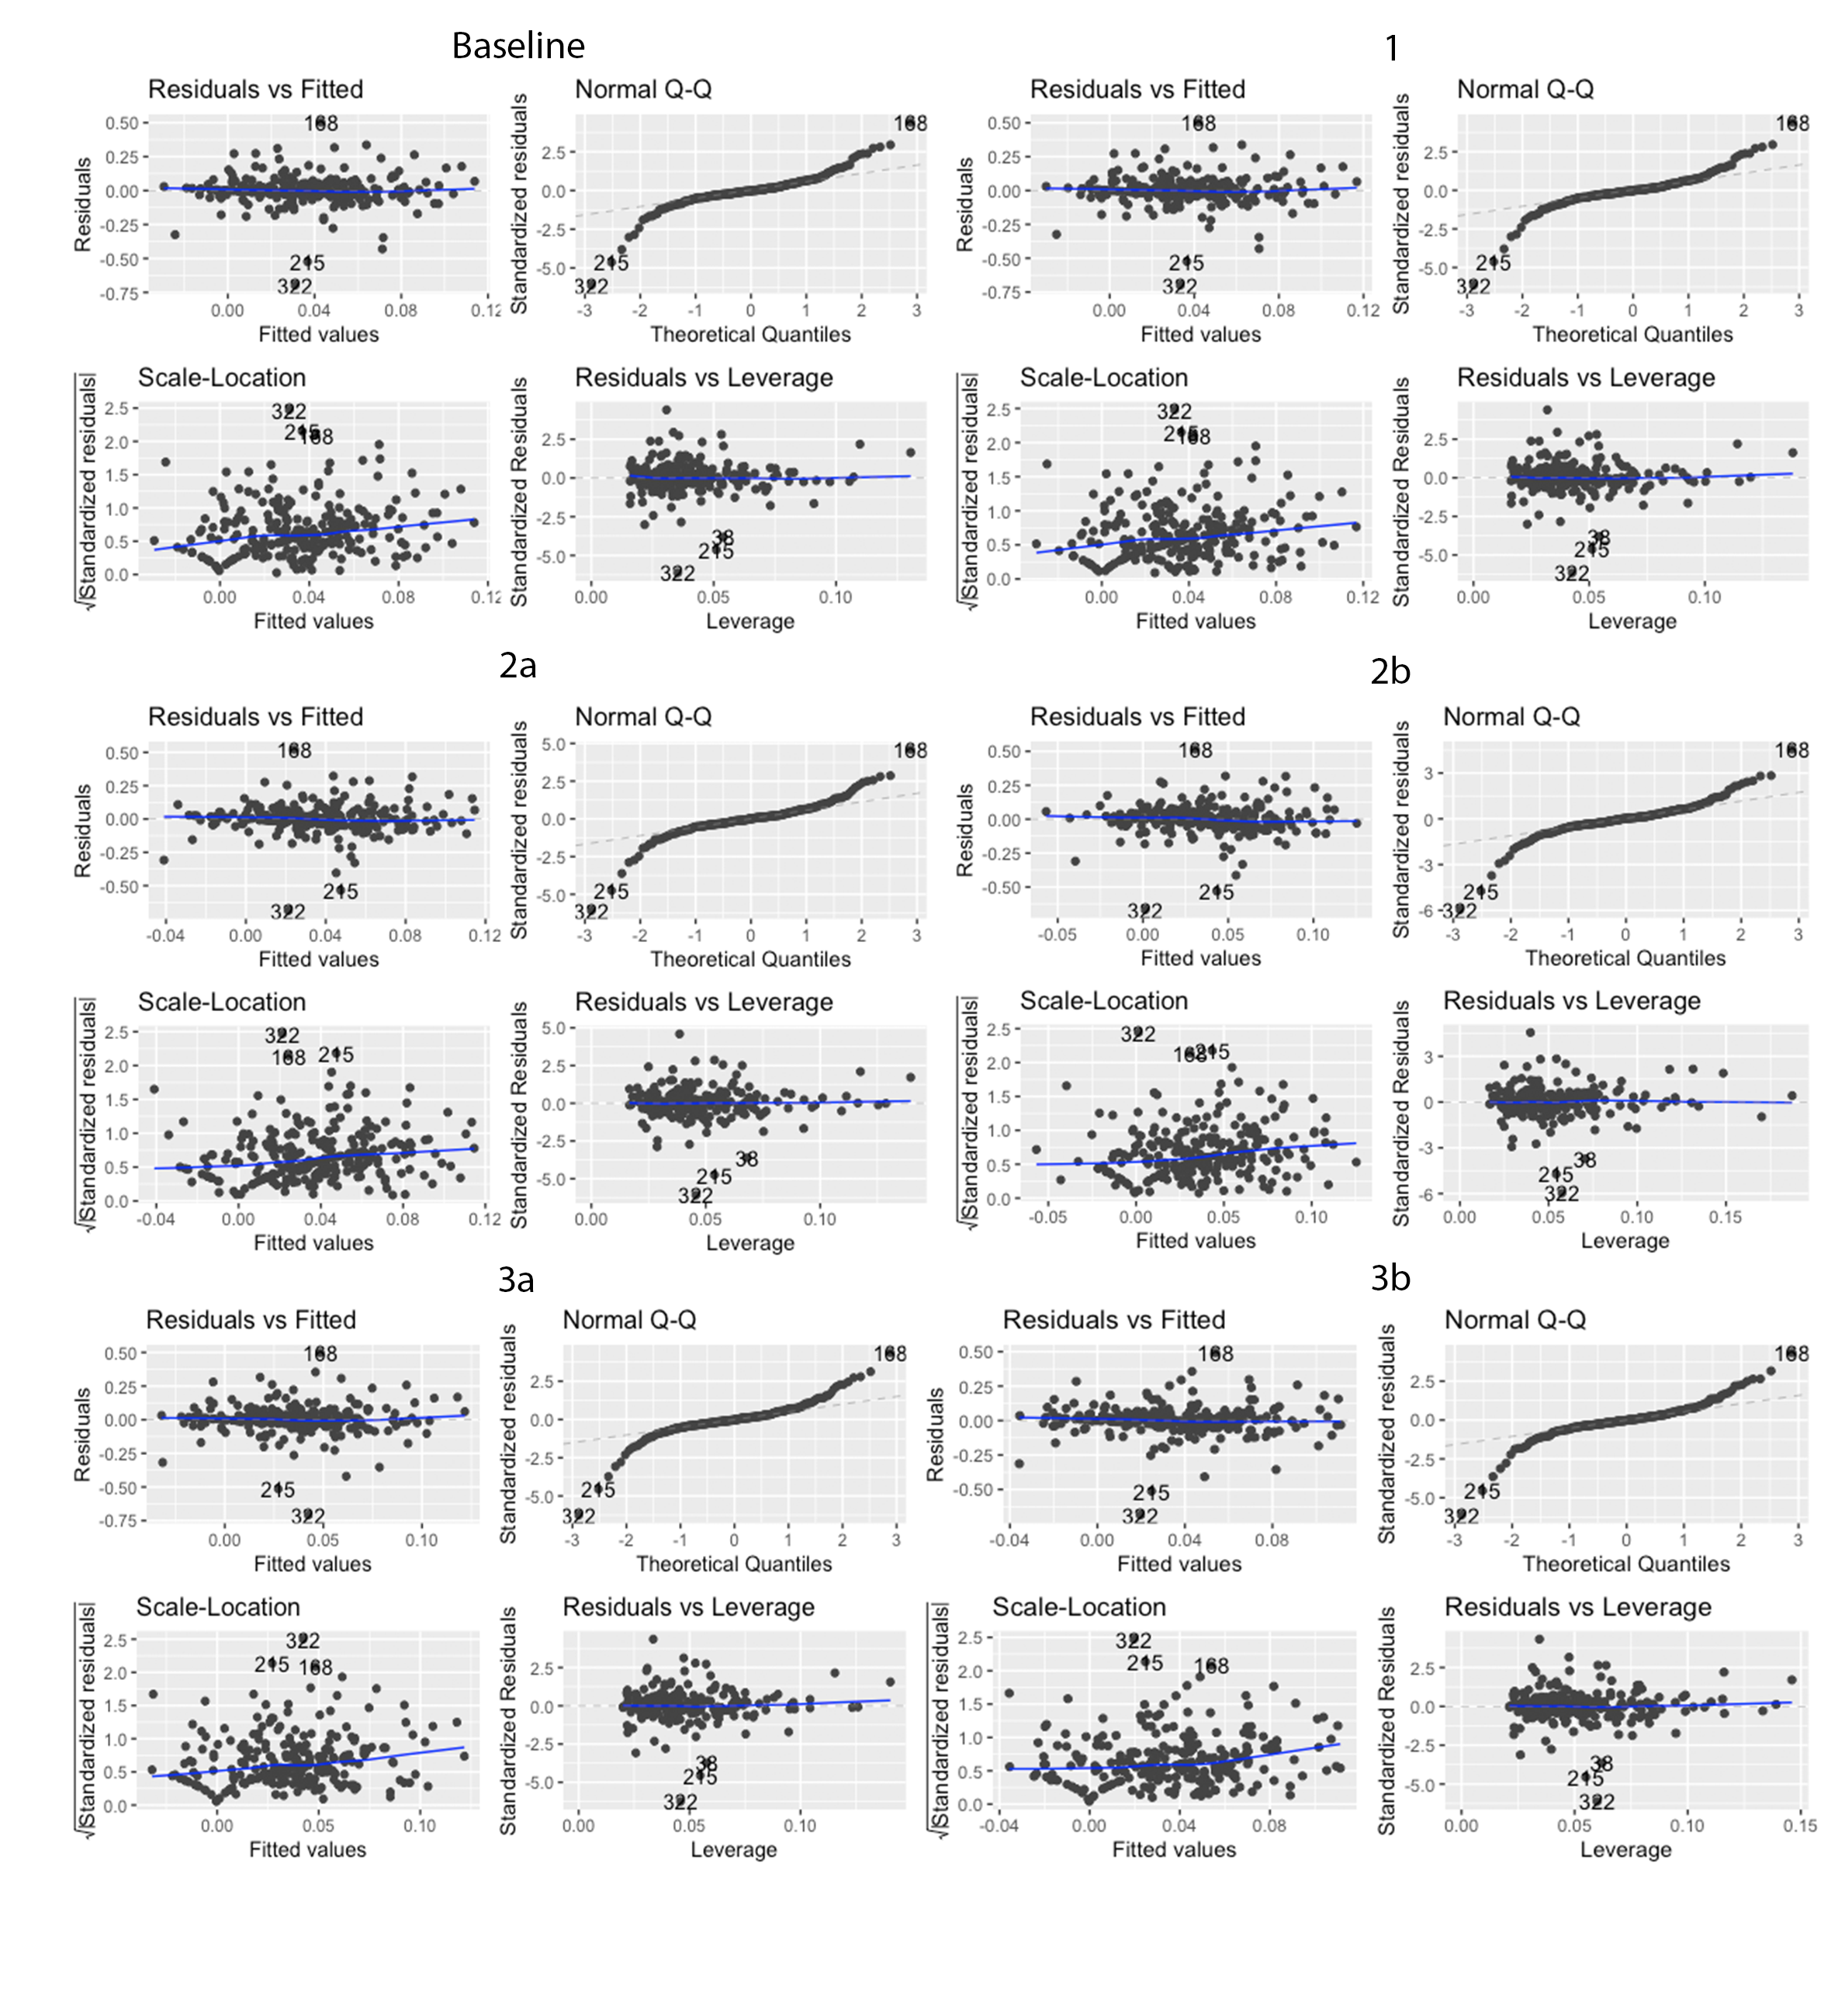
\includegraphics[scale=0.75]{chinchilab-template/Pictures/Model2.2_diag.png}
    \caption*{Diagnostic Plots}%
\end{figure}

\begin{landscape}
\thispagestyle{mylandscape}
\begin{table}[!htbp] \centering 
  \caption*{} 
  \begin{adjustbox}{width=\columnwidth,center}
\begin{tabular}{@{\extracolsep{5pt}}lD{.}{.}{-3} D{.}{.}{-3} D{.}{.}{-3} D{.}{.}{-3} D{.}{.}{-3} D{.}{.}{-3} } 
\\[-1.8ex]\hline 
\hline \\[-1.8ex] 
 & \multicolumn{6}{c}{\textit{Dependent variable:}} \\ 
\cline{2-7} 
\\[-1.8ex] & \multicolumn{6}{c}{EmploymentGrowth} \\ 
\\[-1.8ex] & \multicolumn{1}{c}{(1)} & \multicolumn{1}{c}{(2)} & \multicolumn{1}{c}{(3)} & \multicolumn{1}{c}{(4)} & \multicolumn{1}{c}{(5)} & \multicolumn{1}{c}{(6)}\\ 
\hline \\[-1.8ex] 
  Bribes &  & 0.012 & 0.139 & 0.160 & 0.003 & -0.132 \\ 
  &  & (0.175) & (0.181) & (0.410) & (0.181) & (0.287) \\ 
  PolicyObstacle &  &  & \cellcolor{yellow}-0.030^{**} & \cellcolor{yellow}-0.030^{**} &  &  \\ 
  &  &  & (0.013) & (0.015) &  &  \\ 
  Bribes $\times$ PolicyObstacle &  &  &  & -0.017 &  &  \\ 
  &  &  &  & (0.291) &  &  \\ 
  InformalCompetition &  &  &  &  & 0.004 & -0.002 \\ 
  &  &  &  &  & (0.020) & (0.023) \\ 
  Bribes $\times$ InformalCompetition &  &  &  &  &  & 0.221 \\ 
  &  &  &  &  &  & (0.365) \\ 
 Sector & -0.026 & -0.026 & -0.027 & -0.027 & -0.027 & -0.027 \\ 
  & (0.022) & (0.023) & (0.022) & (0.023) & (0.023) & (0.023) \\ 
  Small & -0.028 & -0.028 & -0.027 & -0.027 & -0.030 & -0.030 \\ 
  & (0.026) & (0.026) & (0.026) & (0.026) & (0.027) & (0.027) \\ 
  Medium & 0.027 & 0.027 & 0.028 & 0.028 & 0.027 & 0.027 \\ 
  & (0.024) & (0.024) & (0.023) & (0.024) & (0.024) & (0.024) \\ 
  lnAge & -0.022 & -0.022 & -0.024 & -0.024 & -0.022 & -0.022 \\ 
  & (0.018) & (0.018) & (0.018) & (0.018) & (0.018) & (0.018) \\ 
  lnExperience & -0.007 & -0.007 & -0.008 & -0.008 & -0.007 & -0.008 \\ 
  & (0.019) & (0.019) & (0.019) & (0.019) & (0.019) & (0.019) \\ 
  Foreign & 0.018 & 0.018 & 0.021 & 0.021 & 0.018 & 0.021 \\ 
  & (0.037) & (0.037) & (0.037) & (0.037) & (0.037) & (0.038) \\ 
  Export & 0.007 & 0.007 & 0.018 & 0.018 & 0.007 & 0.007 \\ 
  & (0.030) & (0.030) & (0.030) & (0.030) & (0.030) & (0.030) \\ 
  TrainingEmployees & -0.012 & -0.012 & -0.012 & -0.012 & -0.012 & -0.014 \\ 
  & (0.019) & (0.020) & (0.020) & (0.020) & (0.020) & (0.020) \\ 
  R\&D & 0.002 & 0.003 & 0.019 & 0.018 & 0.001 & 0.003 \\ 
  & (0.022) & (0.023) & (0.023) & (0.023) & (0.023) & (0.024) \\ 
  Constant & 0.123^{**} & 0.123^{**} & 0.151^{**} & 0.151^{**} & 0.124^{**} & 0.129^{**} \\ 
  & (0.060) & (0.060) & (0.061) & (0.061) & (0.061) & (0.061) \\ 
 \hline \\[-1.8ex] 
Observations & \multicolumn{1}{c}{163} & \multicolumn{1}{c}{163} & \multicolumn{1}{c}{163} & \multicolumn{1}{c}{163} & \multicolumn{1}{c}{163} & \multicolumn{1}{c}{163} \\ 
R$^{2}$ & \multicolumn{1}{c}{0.063} & \multicolumn{1}{c}{0.063} & \multicolumn{1}{c}{0.096} & \multicolumn{1}{c}{0.096} & \multicolumn{1}{c}{0.063} & \multicolumn{1}{c}{0.066} \\ 
Adjusted R$^{2}$ & \multicolumn{1}{c}{0.008} & \multicolumn{1}{c}{0.002} & \multicolumn{1}{c}{0.031} & \multicolumn{1}{c}{0.024} & \multicolumn{1}{c}{-0.005} & \multicolumn{1}{c}{-0.009} \\ 
Residual Std. Error & \multicolumn{1}{c}{0.112 (df = 153)} & \multicolumn{1}{c}{0.113 (df = 152)} & \multicolumn{1}{c}{0.111 (df = 151)} & \multicolumn{1}{c}{0.112 (df = 150)} & \multicolumn{1}{c}{0.113 (df = 151)} & \multicolumn{1}{c}{0.113 (df = 150)} \\ 
F Statistic & \multicolumn{1}{c}{1.146 (df = 9; 153)} & \multicolumn{1}{c}{1.025 (df = 10; 152)} & \multicolumn{1}{c}{1.466 (df = 11; 151)} & \multicolumn{1}{c}{1.335 (df = 12; 150)} & \multicolumn{1}{c}{0.930 (df = 11; 151)} & \multicolumn{1}{c}{0.879 (df = 12; 150)} \\ 
\hline 
\hline \\[-1.8ex] 
\textit{Note:}  & \multicolumn{6}{r}{$^{*}$p$<$0.1; $^{**}$p$<$0.05; $^{***}$p$<$0.01} \\ 
\end{tabular} 
\end{adjustbox}
\end{table}
\end{landscape}

\textbf{\Large Model EBI}

\begin{table}[H] \centering 
  \caption*{Summary Statistics} 
\begin{tabular}{@{\extracolsep{5pt}}lccccccc} 
\\[-1.8ex]\hline 
\hline \\[-1.8ex] 
Statistic & \multicolumn{1}{c}{N} & \multicolumn{1}{c}{Mean} & \multicolumn{1}{c}{St. Dev.} & \multicolumn{1}{c}{Min} & \multicolumn{1}{c}{Pctl(25)} & \multicolumn{1}{c}{Pctl(75)} & \multicolumn{1}{c}{Max} \\ 
\hline \\[-1.8ex] 
EmploymentGrowth & 255 & 0.036 & 0.117 & $-$1 & 0 & 0.1 & 1 \\ 
BribeIndex & 255 & 0.227 & 0.420 & 0 & 0 & 0 & 1 \\ 
InformalCompetition & 255 & 0.498 & 0.501 & 0 & 0 & 1 & 1 \\ 
PolicyObstacle & 255 & 1.107 & 0.794 & 0.000 & 0.500 & 1.750 & 3.500 \\ 
Sector & 255 & 0.427 & 0.496 & 0 & 0 & 1 & 1 \\ 
Small & 255 & 0.373 & 0.484 & 0 & 0 & 1 & 1 \\ 
Medium & 255 & 0.314 & 0.465 & 0 & 0 & 1 & 1 \\ 
Large & 255 & 0.314 & 0.465 & 0 & 0 & 1 & 1 \\ 
lnAge & 255 & 2.665 & 0.557 & 1.386 & 2.350 & 3.135 & 4.454 \\ 
lnExperience & 255 & 2.932 & 0.560 & 0.693 & 2.674 & 3.296 & 3.807 \\ 
Foreign & 255 & 0.084 & 0.270 & 0 & 0 & 0 & 1 \\ 
Export & 255 & 0.250 & 0.408 & 0 & 0 & 0.3 & 1 \\ 
TrainingEmployees & 255 & 0.420 & 0.494 & 0 & 0 & 1 & 1 \\ 
R\&D & 255 & 0.224 & 0.417 & 0 & 0 & 0 & 1 \\ 
\hline \\[-1.8ex] 
\end{tabular} 
\end{table} 

\begin{figure}[H]%
    \centering
    \begin{subfigure}
    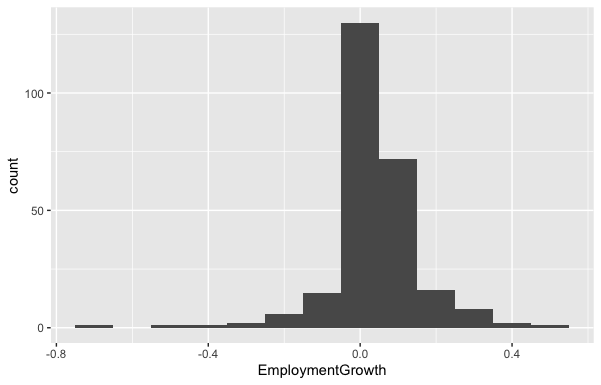
\includegraphics[width=7cm]{chinchilab-template/Pictures/Model2.2_hist_a.png}
    \end{subfigure}
    \begin{subfigure}
    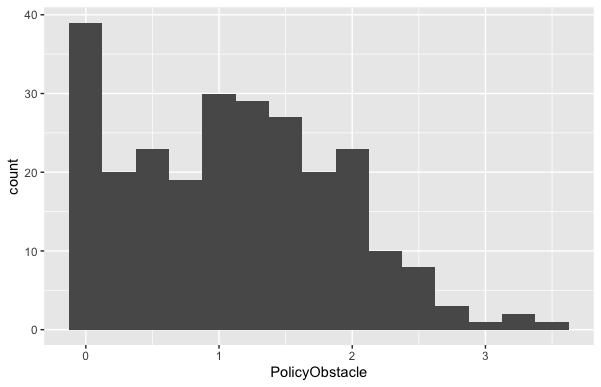
\includegraphics[width=7cm]{chinchilab-template/Pictures/Model2.2_hist_b.png}
    \end{subfigure}
    \begin{subfigure}
    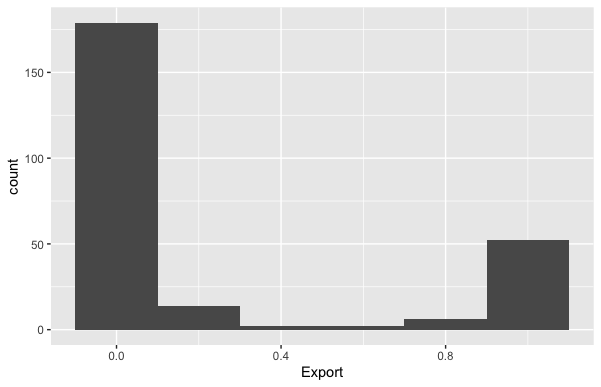
\includegraphics[width=7cm]{chinchilab-template/Pictures/Model2.2_hist_c.png}
    \end{subfigure}
    \begin{subfigure}
    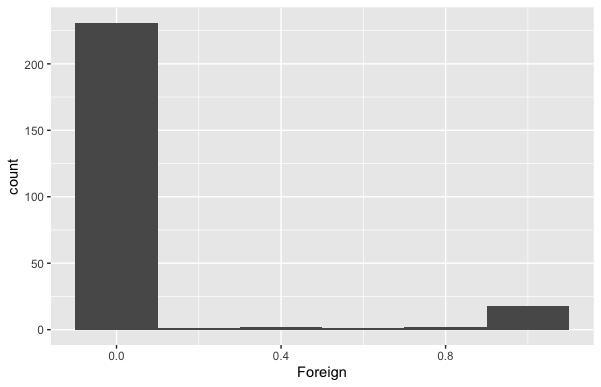
\includegraphics[width=7cm]{chinchilab-template/Pictures/Model2.2_hist_d.png}
    \end{subfigure}
    \caption*{Histogram of Continuous Variables}%
\end{figure}

\begin{figure}[H]
    \centering
    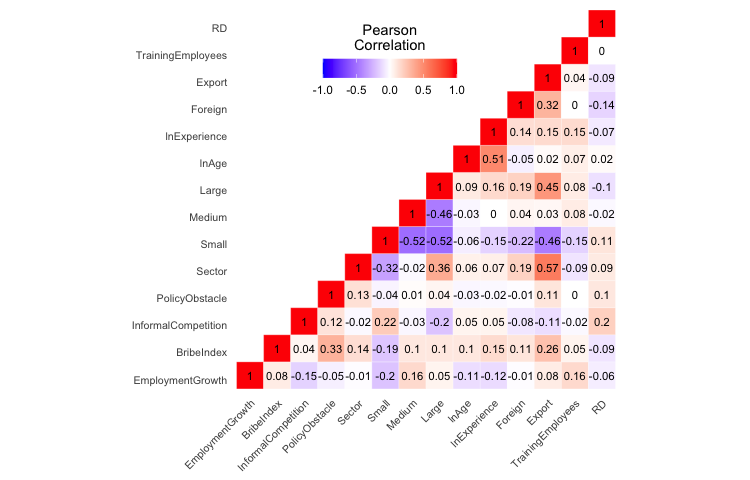
\includegraphics[scale=0.7]{chinchilab-template/Pictures/Model2.2_cor.png}
    \label{fig:my_label}
\end{figure}

\begin{table}[H]
\centering
\scalebox{0.9}{%
\begin{tabular}{lllllll}
\hline
\multicolumn{7}{c}{Variance Inflation Factor (VIF)}                                          \\ \hline
Coefficients                & Baseline & Model 1 & Model 2a & Model 2b & Model 3a & Model 3b \\ \hline
BribeIndex                  &          & 1.09    & 1.21     & 5.88     & 1.10     & 2.29     \\
Policy Obstacle             &          &         & 1.15     & 1.40     &          &          \\
BribeIndex*Policy Obstacle      &          &         &          & 6.79     &          &          \\
Informal Competition        &          &         &          &          & 1.13     & 1.46     \\
BribeIndex*Informal Competition &          &         &          &          &          & 2.61    \\
Sector                      & 1.61     & 1.61    & 1.61     & 1.64     & 1.61     & 1.63     \\
Small                       & 2.05     & 2.05    & 2.06     & 2.06     & 2.14     & 2.14     \\
Medium                      & 1.57     & 1.58    & 1.58     & 1.60     & 1.59     & 1.60     \\
lnAge                       & 1.33     & 1.35    & 1.35     & 1.35     & 1.35     & 1.37     \\
lnExperience                & 1.37     & 1.37    & 1.37     & 1.38     & 1.38     & 1.40     \\
Foreign                     & 1.21     & 1.21    & 1.21     & 1.22     & 1.21     & 1.21     \\
Export                      & 2.01     & 2.06    & 2.07     & 2.14     & 2.07     & 2.07     \\
TrainingEmployees           & 1.08     & 1.08    & 1.08     & 1.09     & 1.08     & 1.09     \\
R\&D                        & 1.10     & 1.10    & 1.12     & 1.12     & 1.13     & 1.14     
\end{tabular}}
\end{table}

\begin{figure}[!h]%
    \centering
    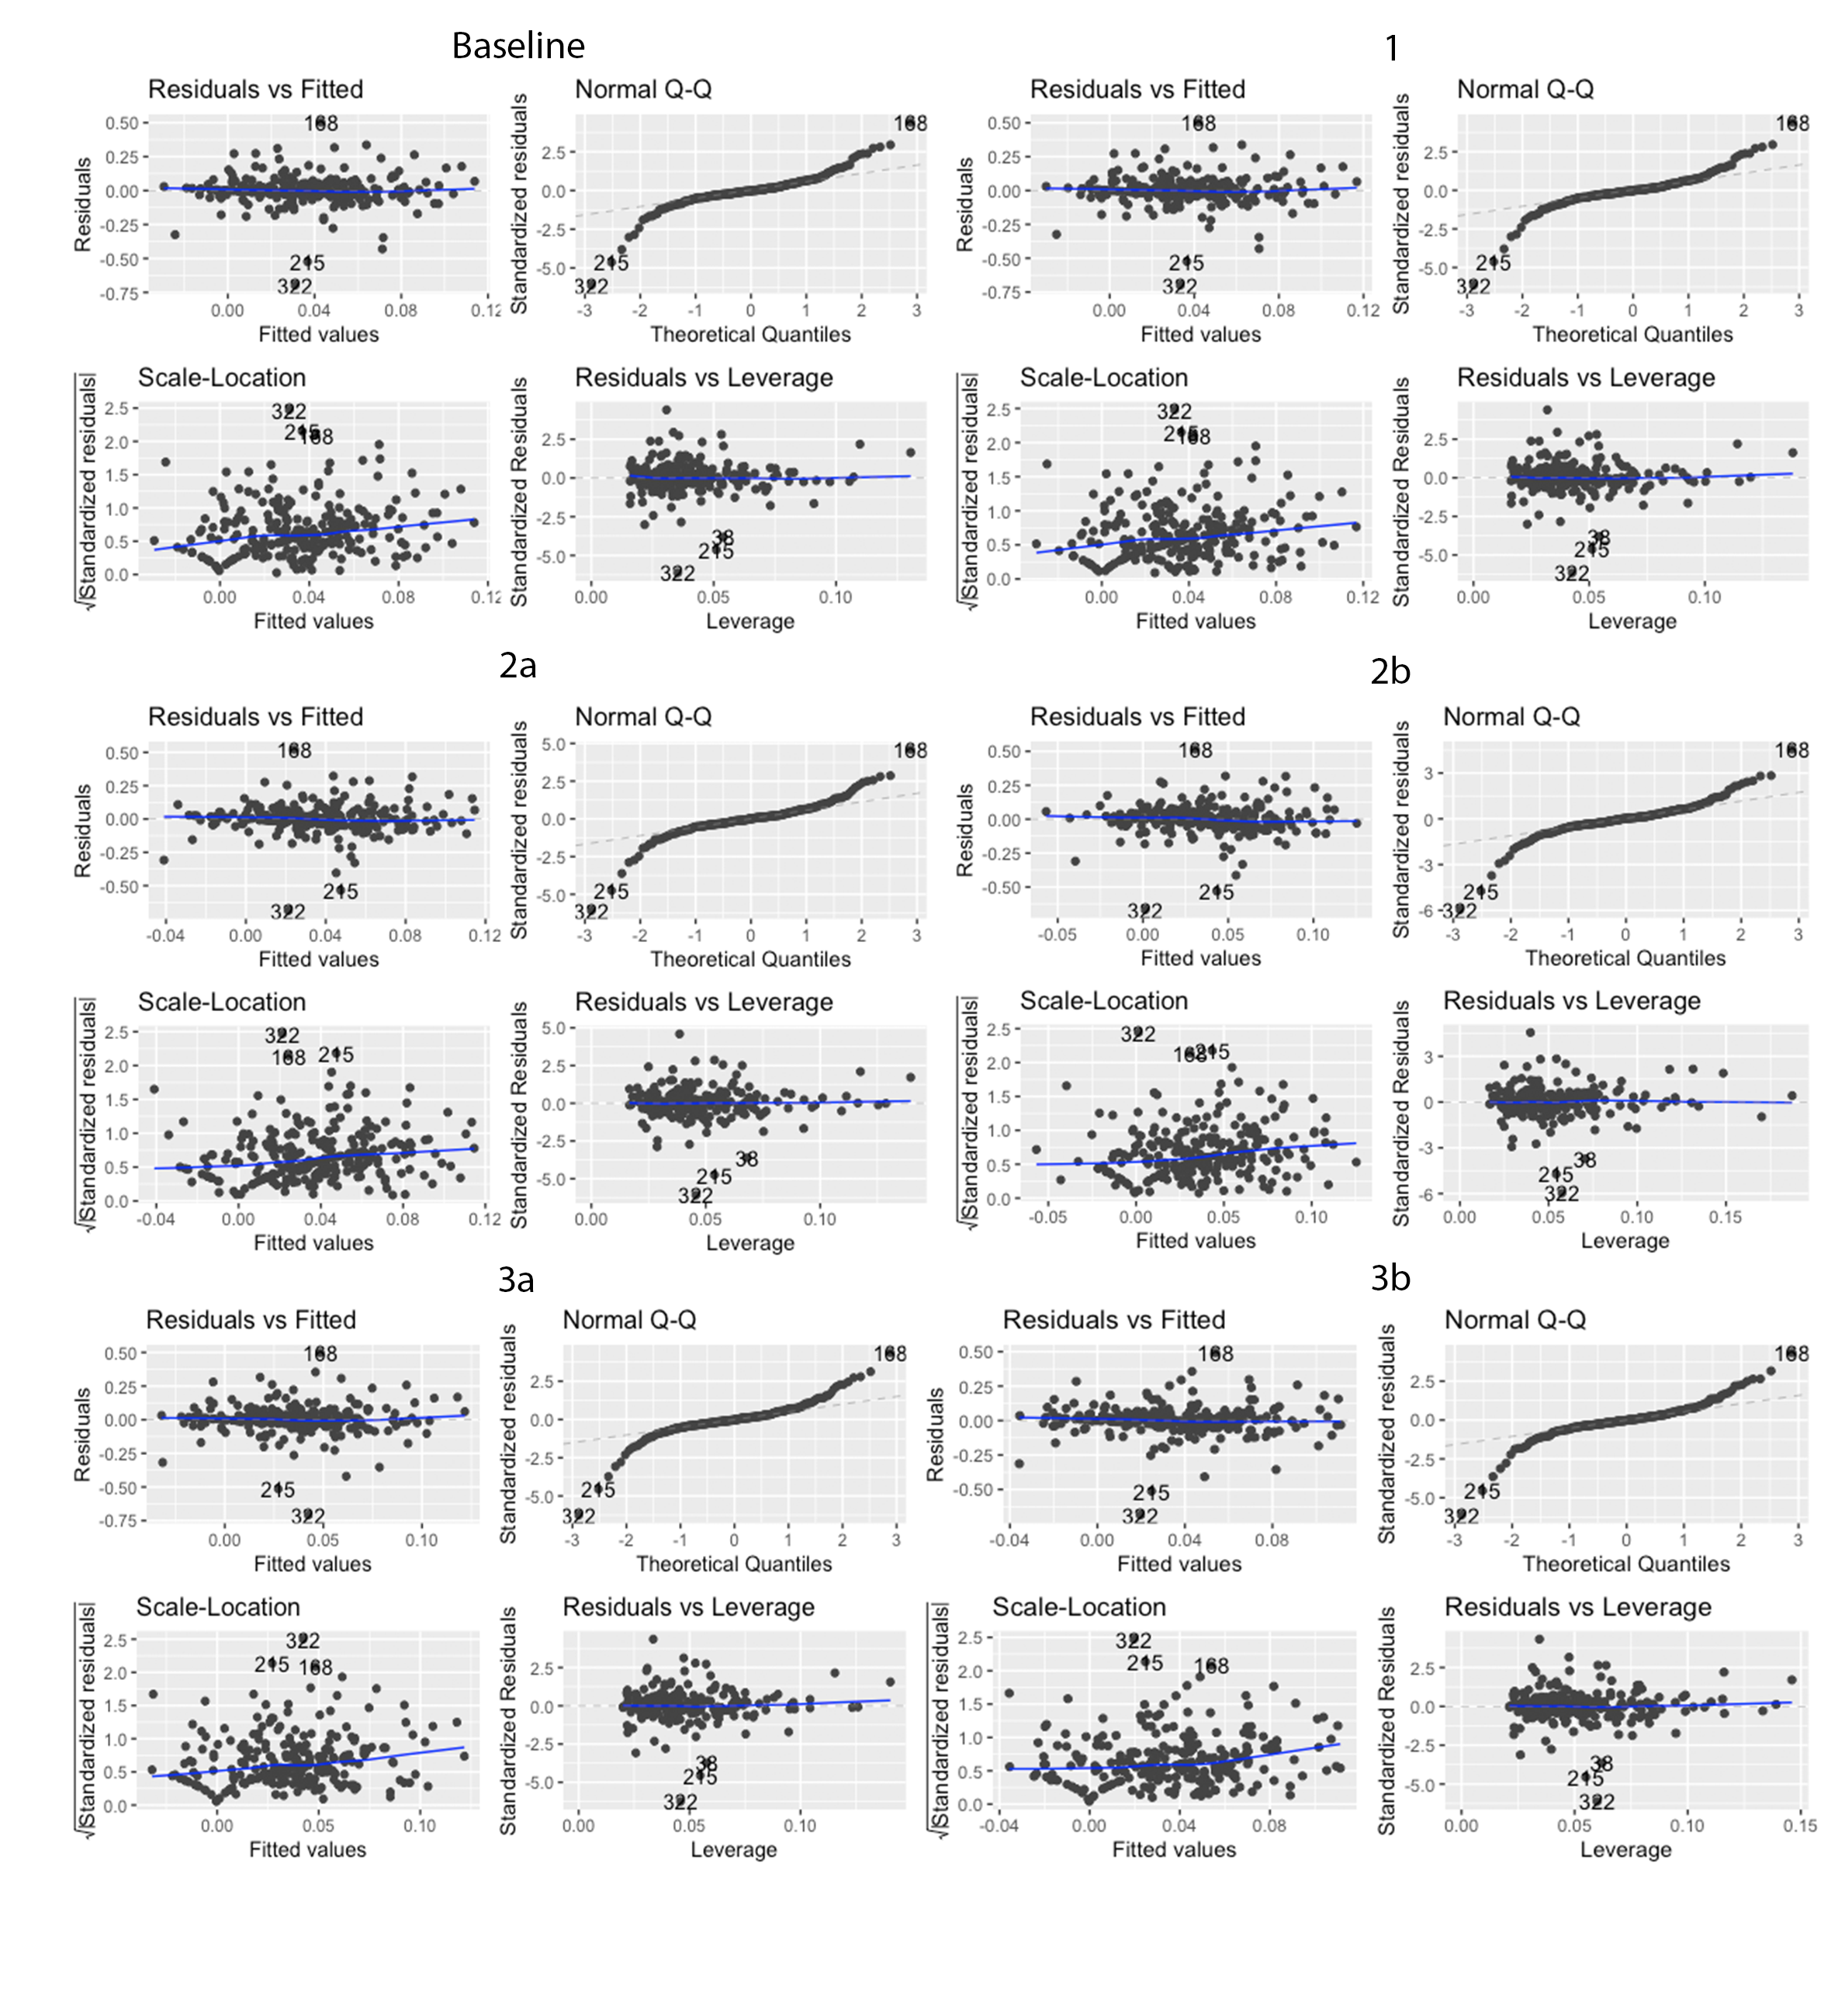
\includegraphics[scale=0.75]{chinchilab-template/Pictures/Model2.2_diag.png}
    \caption*{Diagnostic Plots}%
\end{figure}
\clearpage
\newpage

\textbf{\Large Model EIB}

\begin{table}[H] \centering 
  \caption*{Summary Statistics} 
\begin{tabular}{@{\extracolsep{5pt}}lccccccc} 
\\[-1.8ex]\hline 
\hline \\[-1.8ex] 
Statistic & \multicolumn{1}{c}{N} & \multicolumn{1}{c}{Mean} & \multicolumn{1}{c}{St. Dev.} & \multicolumn{1}{c}{Min} & \multicolumn{1}{c}{Pctl(25)} & \multicolumn{1}{c}{Pctl(75)} & \multicolumn{1}{c}{Max} \\ 
\hline \\[-1.8ex] 
EmploymentGrowth & 236 & 0.039 & 0.115 & $-$1 & 0 & 0.1 & 1 \\ 
Inspection.Bribe & 236 & 0.339 & 0.474 & 0 & 0 & 1 & 1 \\ 
InformalCompetition & 236 & 0.496 & 0.501 & 0 & 0 & 1 & 1 \\ 
PolicyObstacle & 236 & 1.112 & 0.797 & 0.000 & 0.500 & 1.750 & 3.500 \\ 
Sector & 236 & 0.428 & 0.496 & 0 & 0 & 1 & 1 \\ 
Small & 236 & 0.373 & 0.485 & 0 & 0 & 1 & 1 \\ 
Medium & 236 & 0.309 & 0.463 & 0 & 0 & 1 & 1 \\ 
Large & 236 & 0.318 & 0.467 & 0 & 0 & 1 & 1 \\ 
lnAge & 236 & 2.665 & 0.554 & 1.386 & 2.398 & 3.135 & 4.454 \\ 
lnExperience & 236 & 2.937 & 0.549 & 0.693 & 2.691 & 3.268 & 3.807 \\ 
Foreign & 236 & 0.074 & 0.258 & 0 & 0 & 0 & 1 \\ 
Export & 236 & 0.247 & 0.407 & 0 & 0 & 0.3 & 1 \\ 
TrainingEmployees & 236 & 0.441 & 0.498 & 0 & 0 & 1 & 1 \\ 
R\&D & 236 & 0.242 & 0.429 & 0 & 0 & 0 & 1 \\ 
\hline \\[-1.8ex] 
\end{tabular} 
\end{table} 

\begin{figure}[H]%
    \centering
    \begin{subfigure}
    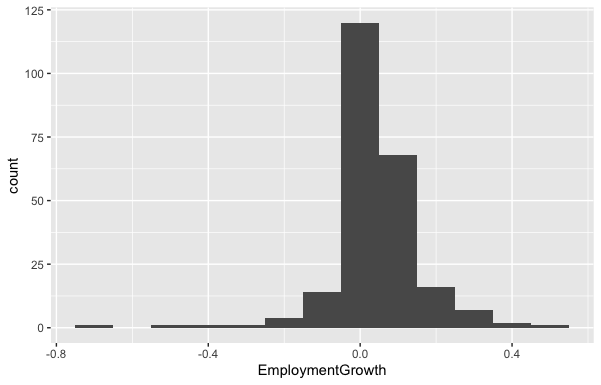
\includegraphics[width=7cm]{chinchilab-template/Pictures/Model2.3_hist_a.png}
    \end{subfigure}
    \begin{subfigure}
    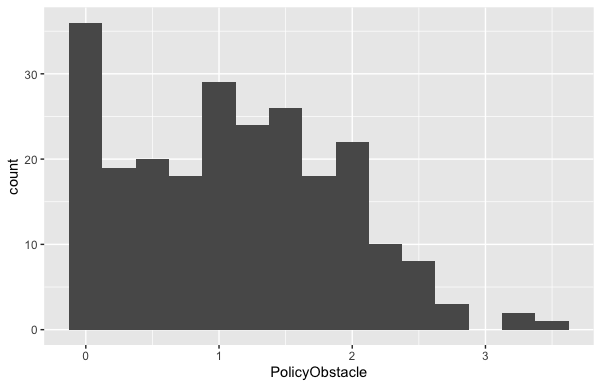
\includegraphics[width=7cm]{chinchilab-template/Pictures/Model2.3_hist_b.png}
    \end{subfigure}
    \begin{subfigure}
    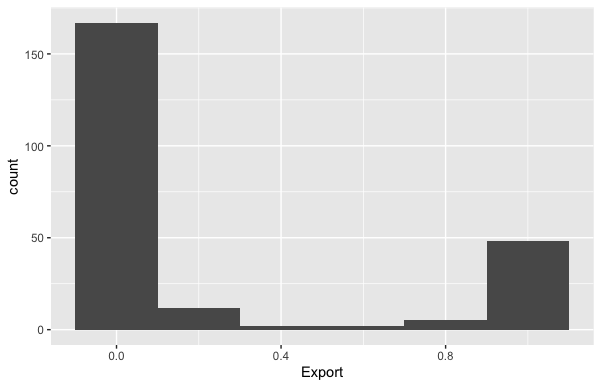
\includegraphics[width=7cm]{chinchilab-template/Pictures/Model2.3_hist_c.png}
    \end{subfigure}
    \begin{subfigure}
    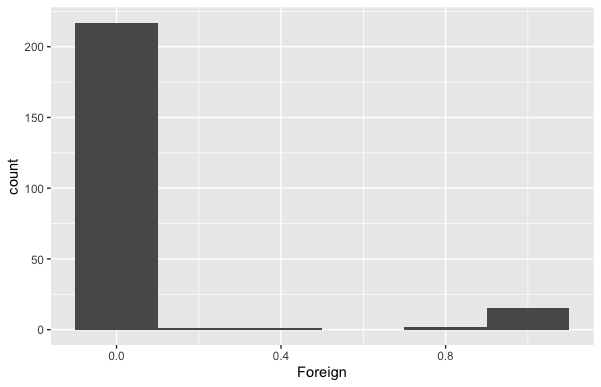
\includegraphics[width=7cm]{chinchilab-template/Pictures/Model2.3_hist_d.png}
    \end{subfigure}
    \caption*{Histogram of Continuous Variables}%
\end{figure}

\begin{figure}[H]
    \centering
    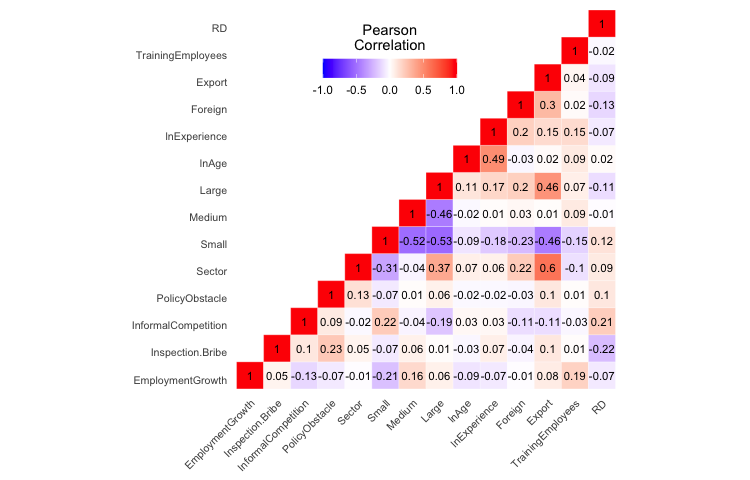
\includegraphics[scale=0.7]{chinchilab-template/Pictures/Model2.3_cor.png}
    \label{fig:my_label}
\end{figure}

\begin{table}[H]
\centering
\scalebox{0.9}{%
\begin{tabular}{lllllll}
\hline
\multicolumn{7}{c}{Variance Inflation Factor (VIF)}                                          \\ \hline
Coefficients                & Baseline & Model 1 & Model 2a & Model 2b & Model 3a & Model 3b \\ \hline
Inspection.Bribe            &          & 1.08    & 1.15     & 3.84     & 1.10     & 2.22     \\
Policy Obstacle             &          &         & 1.11     & 1.70     &          &          \\
Inspection.Bribe*Policy Obstacle      &          &         &          & 4.95     &          &          \\
Informal Competition        &          &         &          &          & 1.14     & 1.76     \\
Inspection.Bribe*Informal Competition &          &         &          &          &          & 3.01  \\
Sector                      & 1.66     & 1.67    & 1.68     & 1.71     & 1.68     & 1.68     \\
Small                       & 2.08     & 2.08    & 2.08     & 2.08     & 2.15     & 2.15     \\
Medium                      & 1.59     & 1.59    & 1.59     & 1.60     & 1.60     & 1.60     \\
lnAge                       & 1.33     & 1.34    & 1.34     & 1.36     & 1.35     & 1.35     \\
lnExperience                & 1.37     & 1.38    & 1.39     & 1.39     & 1.38     & 1.39     \\
Foreign                     & 1.21     & 1.23    & 1.23     & 1.23     & 1.23     & 1.23     \\
Export                      & 2.06     & 2.06    & 2.07     & 2.11     & 2.06     & 2.06     \\
TrainingEmployees           & 1.08     & 1.08    & 1.08     & 1.10     & 1.08     & 1.12     \\
R\&D                        & 1.11     & 1.17    & 1.20     & 1.21     & 1.22     & 1.26     \\
\end{tabular}}
\end{table}

\begin{figure}[!t]%
    \centering
    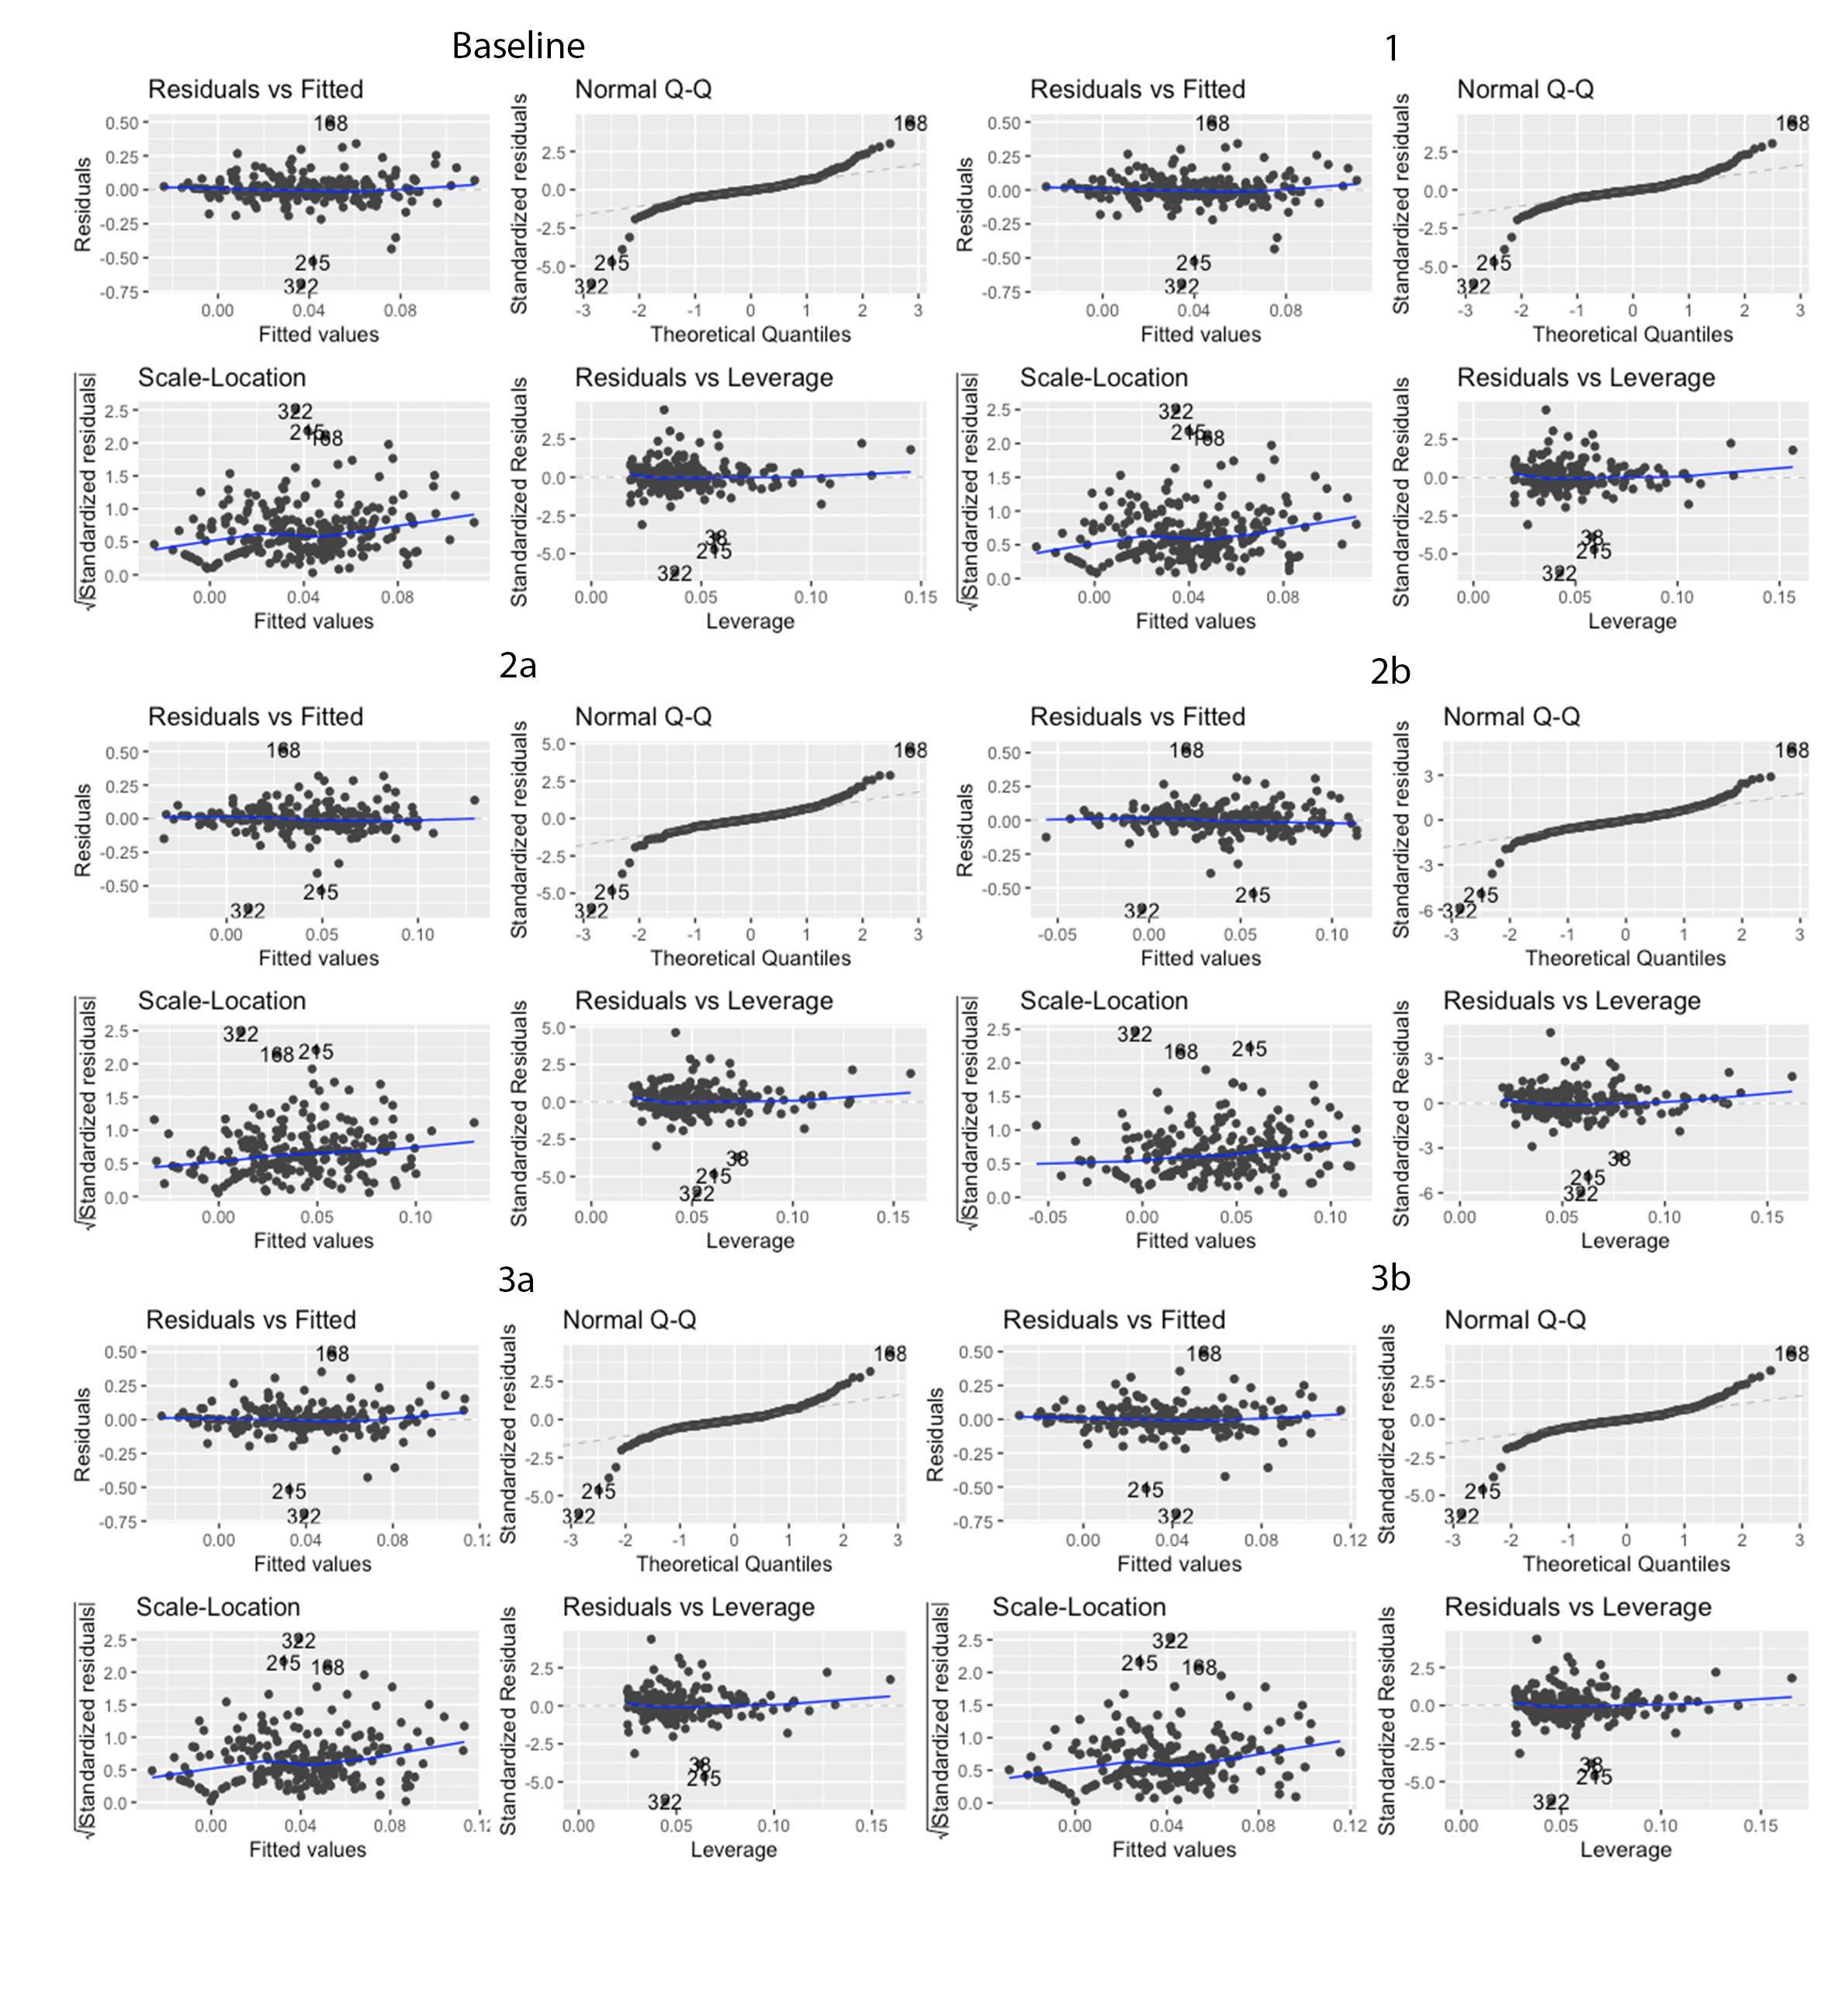
\includegraphics[scale=0.75]{chinchilab-template/Pictures/Model2.3_diag.png}
    \caption*{Diagnostic Plots}%
\end{figure}
\clearpage
\newpage

\textbf{\Large Model LB}
\begin{table}[H] \centering 
  \caption*{} 
  \scalebox{0.8}{%
\begin{tabular}{@{\extracolsep{5pt}}lccccccc} 
\\[-1.8ex]\hline 
\hline \\[-1.8ex] 
Statistic & \multicolumn{1}{c}{N} & \multicolumn{1}{c}{Mean} & \multicolumn{1}{c}{St. Dev.} & \multicolumn{1}{c}{Min} & \multicolumn{1}{c}{Pctl(25)} & \multicolumn{1}{c}{Pctl(75)} & \multicolumn{1}{c}{Max} \\ 
\hline \\[-1.8ex] 
LaborProductivityGrowth & 156 & 0.058 & 0.286 & $-$0.665 & $-$0.068 & 0.148 & 0.667 \\ 
Bribes & 156 & 0.029 & 0.053 & 0.000 & 0.000 & 0.050 & 0.200 \\ 
InformalCompetition & 156 & 0.538 & 0.500 & 0 & 0 & 1 & 1 \\ 
PolicyObstacle & 156 & 0.984 & 0.742 & 0 & 0.2 & 1.5 & 4 \\ 
Sector & 156 & 0.429 & 0.497 & 0 & 0 & 1 & 1 \\ 
Small & 156 & 0.378 & 0.487 & 0 & 0 & 1 & 1 \\ 
Medium & 156 & 0.288 & 0.455 & 0 & 0 & 1 & 1 \\ 
Large & 156 & 0.333 & 0.473 & 0 & 0 & 1 & 1 \\ 
lnAge & 156 & 2.622 & 0.558 & 1.386 & 2.276 & 3.102 & 3.367 \\ 
lnExperience & 156 & 2.933 & 0.539 & 1.099 & 2.691 & 3.258 & 3.807 \\ 
Foreign & 156 & 0.087 & 0.271 & 0 & 0 & 0 & 1 \\ 
Export & 156 & 0.264 & 0.415 & 0 & 0 & 0.4 & 1 \\ 
TrainingEmployees & 156 & 0.365 & 0.483 & 0 & 0 & 1 & 1 \\ 
R\&D & 156 & 0.231 & 0.423 & 0 & 0 & 0 & 1 \\ 
\hline \\[-1.8ex] 
\end{tabular}}
\end{table} 

\begin{figure}[H]%
    \centering
    \begin{subfigure}
    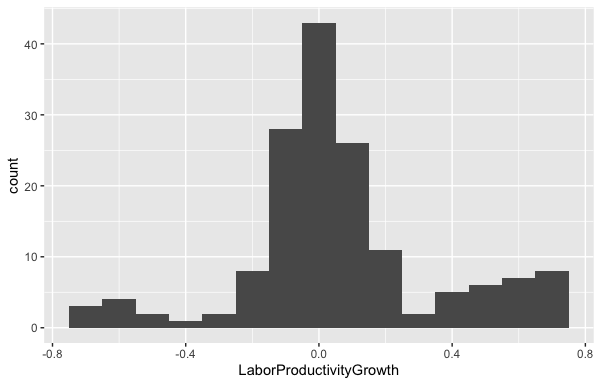
\includegraphics[width=7cm]{chinchilab-template/Pictures/Model3_hist_a.png}
    \end{subfigure}
    \begin{subfigure}
    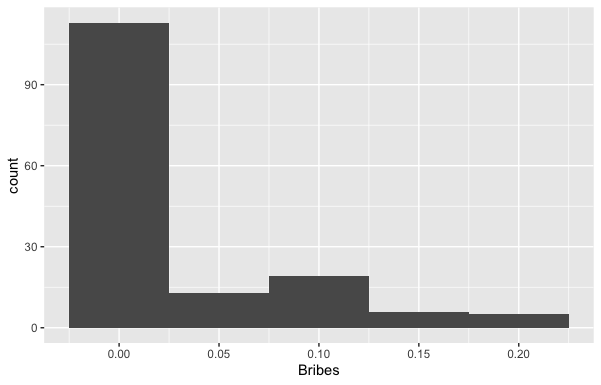
\includegraphics[width=7cm]{chinchilab-template/Pictures/Model3_hist_b.png}
    \end{subfigure}
    \begin{subfigure}
    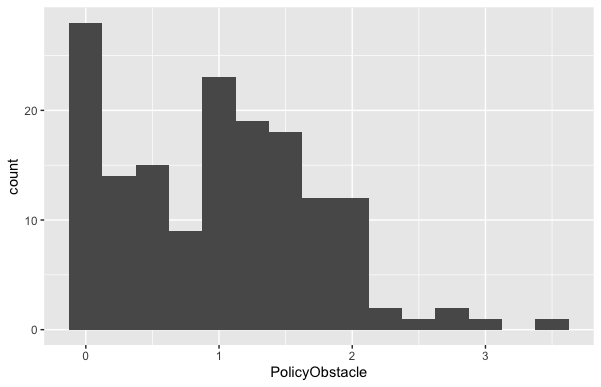
\includegraphics[width=7cm]{chinchilab-template/Pictures/Model3_hist_c.png}
    \end{subfigure}
    \begin{subfigure}
    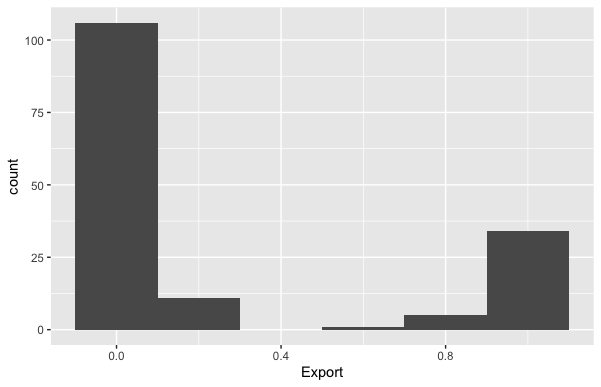
\includegraphics[width=7cm]{chinchilab-template/Pictures/Model3_hist_d.png}
    \end{subfigure}
    \begin{subfigure}
    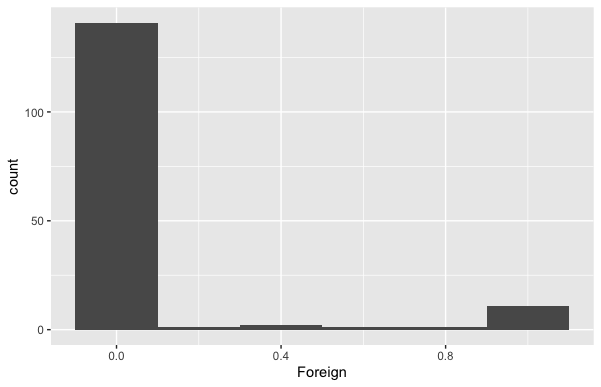
\includegraphics[width=7cm]{chinchilab-template/Pictures/Model3_hist_e.png}
    \end{subfigure}
    \caption*{Histogram of Continuous Variables}%
\end{figure}

\begin{figure}[H]
    \centering
    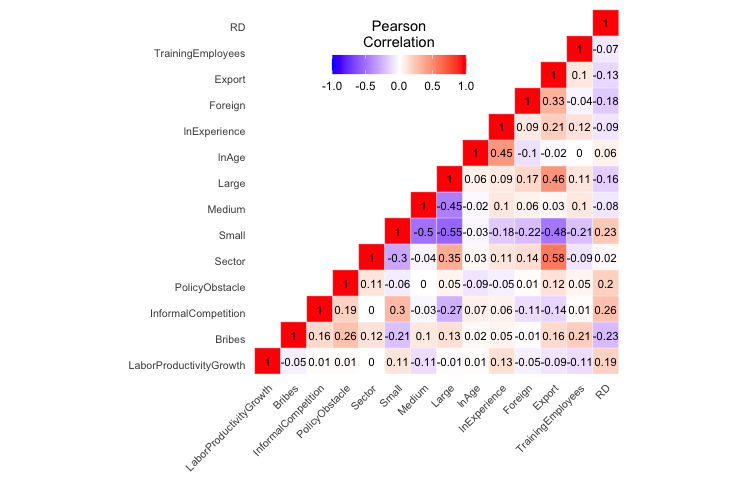
\includegraphics[scale=0.7]{chinchilab-template/Pictures/Model3_cor.png}
    \label{fig:my_label}
\end{figure}

\begin{table}[H]
\centering
\scalebox{0.9}{%
\begin{tabular}{lllllll}
\hline
\multicolumn{7}{c}{Variance Inflation Factor (VIF)}                                          \\ \hline
Coefficients                & Baseline & Model 1 & Model 2a & Model 2b & Model 3a & Model 3b \\ \hline
Bribes                      &          & 1.12    & 1.24     & 6.32     & 1.23     & 3.62     \\
Policy Obstacle             &          &         & 1.22     & 1.59     &          &          \\
Bribes*Policy Obstacle      &          &         &          & 7.36     &          &          \\
Informal Competition        &          &         &          &          & 1.32     & 1.63     \\
Bribes*Informal Competition &          &         &          &          &          & 4.28  \\
Sector                      & 1.57     & 1.57    & 1.57     & 1.60     & 1.60     & 1.60     \\
Small                       & 2.04     & 2.04    & 2.04     & 2.08     & 2.26     & 2.26     \\
Medium                      & 1.49     & 1.49    & 1.50     & 1.53     & 1.53     & 1.53     \\
lnAge                       & 1.28     & 1.28    & 1.29     & 1.29     & 1.29     & 1.30     \\
lnExperience                & 1.33     & 1.33    & 1.33     & 1.34     & 1.34     & 1.38     \\
Foreign                     & 1.24     & 1.25    & 1.25     & 1.27     & 1.25     & 1.28     \\
Export                      & 2.06     & 2.07    & 2.11     & 2.13     & 2.08     & 2.08     \\
TrainingEmployees           & 1.11     & 1.15    & 1.15     & 1.16     & 1.15     & 1.16     \\
R\&D                        & 1.14     & 1.19    & 1.30     & 1.31     & 1.26     & 1.28     
\end{tabular}}
\end{table}

\begin{figure}[H]%
    \centering
    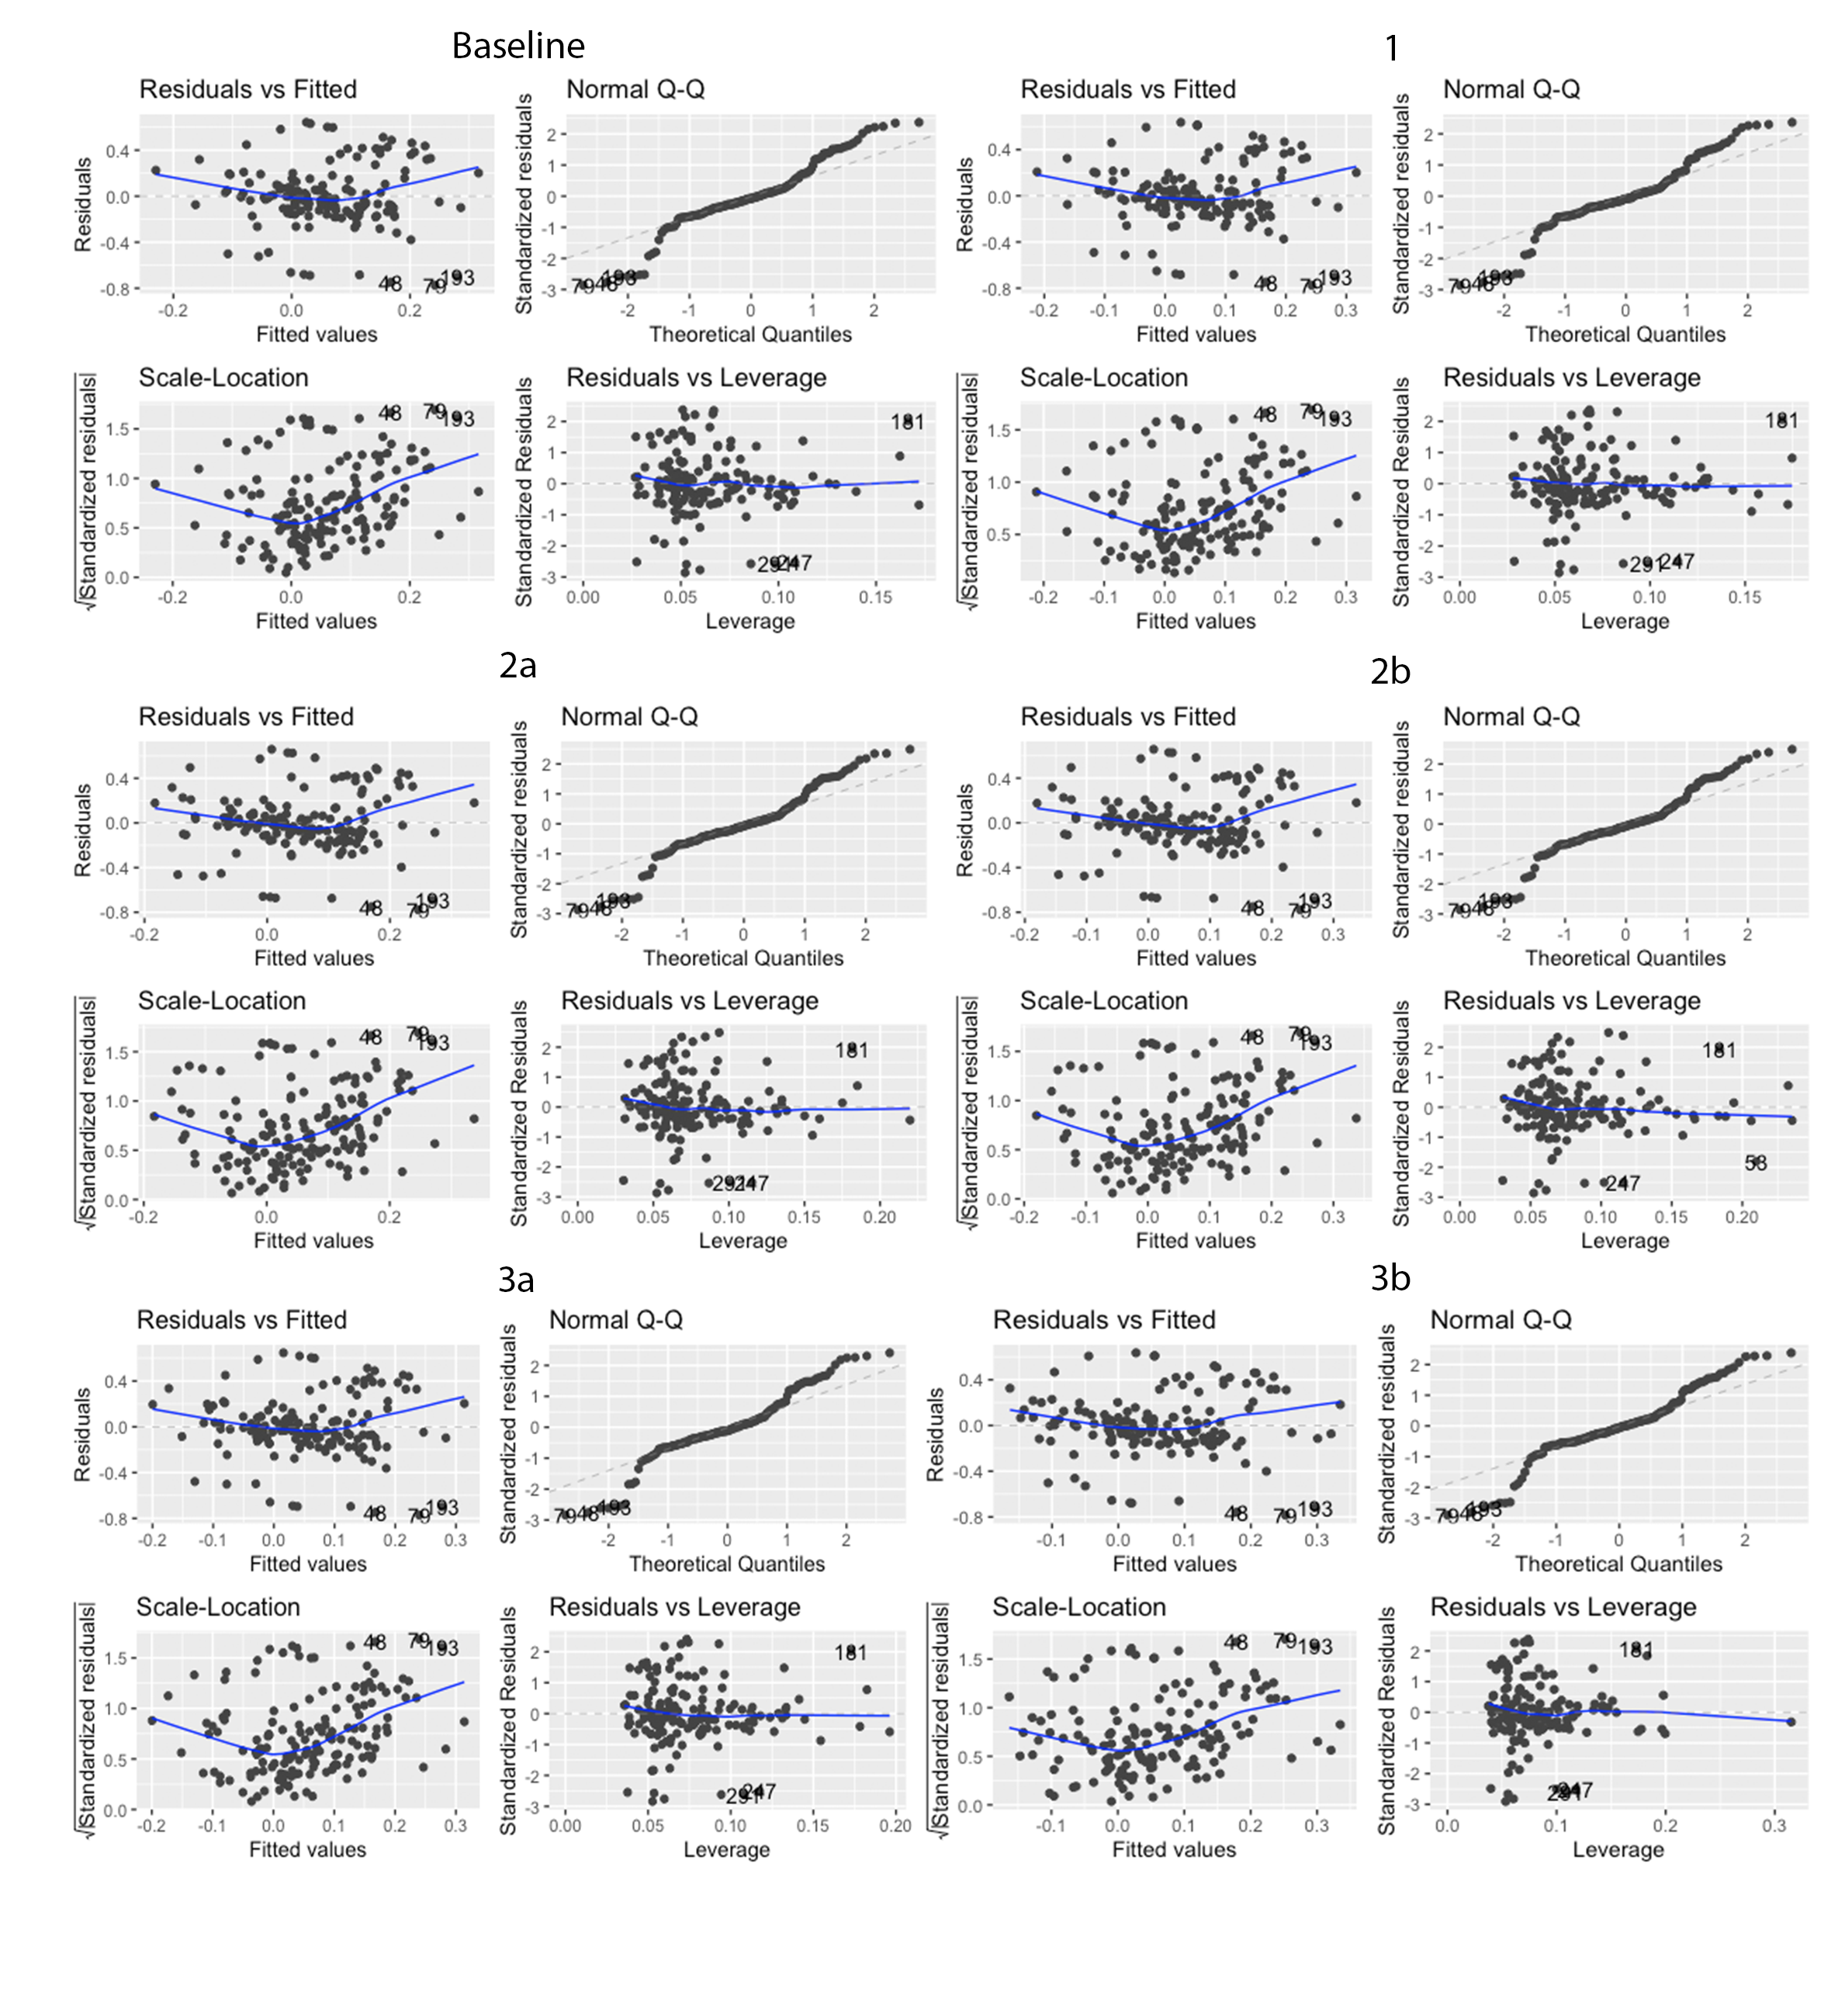
\includegraphics[scale=0.75]{chinchilab-template/Pictures/Model3_diag.png}
    \caption*{Diagnostic Plots}%
\end{figure}

\begin{landscape}
\thispagestyle{mylandscape}
\begin{table}[] \centering 
  \caption*{Summary Statistics} 
  \begin{adjustbox}{width=\columnwidth,center}
\begin{tabular}{@{\extracolsep{5pt}}lD{.}{.}{-3} D{.}{.}{-3} D{.}{.}{-3} D{.}{.}{-3} D{.}{.}{-3} D{.}{.}{-3} } 
\\[-1.8ex]\hline 
\hline \\[-1.8ex] 
 & \multicolumn{6}{c}{\textit{Dependent variable:}} \\ 
\cline{2-7} 
\\[-1.8ex] & \multicolumn{6}{c}{LaborProductivityGrowth} \\ 
\\[-1.8ex] & \multicolumn{1}{c}{(1)} & \multicolumn{1}{c}{(2)} & \multicolumn{1}{c}{(3)} & \multicolumn{1}{c}{(4)} & \multicolumn{1}{c}{(5)} & \multicolumn{1}{c}{(6)}\\ 
\hline \\[-1.8ex] 
  Bribes &  & 0.254 & 0.404 & 0.447 & 0.323 & \cellcolor{yellow}1.406^{*} \\ 
  &  & (0.449) & (0.472) & (1.068) & (0.470) & (0.803) \\ 
  PolicyObstacle &  &  & -0.034 & -0.033 &  &  \\ 
  &  &  & (0.033) & (0.038) &  &  \\ 
  Bribes $\times$ PolicyObstacle &  &  &  & -0.033 &  &  \\ 
  &  &  &  & (0.740) &  &  \\ 
  InformalCompetition &  &  &  &  & -0.026 & 0.015 \\ 
  &  &  &  &  & (0.052) & (0.057) \\ 
  Bribes $\times$ InformalCompetition &  &  &  &  &  & \cellcolor{yellow}-1.613^{*} \\ 
  &  &  &  &  &  & (0.972) \\ 
 Sector & -0.075 & -0.076 & -0.076 & -0.076 & -0.072 & -0.073 \\ 
  & (0.056) & (0.056) & (0.056) & (0.057) & (0.057) & (0.057) \\ 
  Small & -0.007 & -0.005 & -0.005 & -0.005 & 0.006 & 0.011 \\ 
  & (0.065) & (0.066) & (0.066) & (0.067) & (0.069) & (0.069) \\ 
  Medium & -0.040 & -0.040 & -0.039 & -0.040 & -0.035 & -0.035 \\ 
  & (0.060) & (0.060) & (0.060) & (0.061) & (0.061) & (0.061) \\ 
  lnAge & -0.037 & -0.038 & -0.041 & -0.041 & -0.037 & -0.045 \\ 
  & (0.045) & (0.045) & (0.046) & (0.046) & (0.046) & (0.046) \\ 
  lnExperience & \cellcolor{yellow}0.145^{***} & \cellcolor{yellow}0.145^{***} & \cellcolor{yellow}0.144^{***} & \cellcolor{yellow}0.144^{***} & \cellcolor{yellow}0.147^{***} & \cellcolor{yellow}0.161^{***} \\ 
  & (0.048) & (0.048) & (0.048) & (0.048) & (0.048) & (0.049) \\ 
  Foreign & -0.018 & -0.014 & -0.010 & -0.011 & -0.012 & -0.034 \\ 
  & (0.092) & (0.092) & (0.092) & (0.093) & (0.092) & (0.093) \\ 
  Export & 0.062 & 0.060 & 0.072 & 0.072 & 0.058 & 0.061 \\ 
  & (0.077) & (0.077) & (0.078) & (0.079) & (0.078) & (0.077) \\ 
  TrainingEmployees & \cellcolor{yellow}-0.104^{**} & \cellcolor{yellow}-0.108^{**} & \cellcolor{yellow}-0.108^{**} & \cellcolor{yellow}-0.108^{**} & \cellcolor{yellow}-0.107^{**} & \cellcolor{yellow}-0.100^{**} \\ 
  & (0.049) & (0.050) & (0.050) & (0.050) & (0.050) & (0.050) \\ 
  R\&D & \cellcolor{yellow}0.129^{**} & \cellcolor{yellow}0.135^{**} & \cellcolor{yellow}0.154^{**} & \cellcolor{yellow}0.154^{**} & \cellcolor{yellow}0.143^{**} & \cellcolor{yellow}0.131^{**} \\ 
  & (0.056) & (0.058) & (0.060) & (0.061) & (0.060) & (0.060) \\ 
  Constant & -0.232 & -0.237 & -0.204 & -0.204 & -0.241 & -0.282^{*} \\ 
  & (0.151) & (0.151) & (0.155) & (0.155) & (0.152) & (0.153) \\ 
 \hline \\[-1.8ex] 
Observations & \multicolumn{1}{c}{156} & \multicolumn{1}{c}{156} & \multicolumn{1}{c}{156} & \multicolumn{1}{c}{156} & \multicolumn{1}{c}{156} & \multicolumn{1}{c}{156} \\ 
R$^{2}$ & \multicolumn{1}{c}{0.110} & \multicolumn{1}{c}{0.112} & \multicolumn{1}{c}{0.119} & \multicolumn{1}{c}{0.119} & \multicolumn{1}{c}{0.114} & \multicolumn{1}{c}{0.130} \\ 
Adjusted R$^{2}$ & \multicolumn{1}{c}{0.055} & \multicolumn{1}{c}{0.051} & \multicolumn{1}{c}{0.051} & \multicolumn{1}{c}{0.045} & \multicolumn{1}{c}{0.046} & \multicolumn{1}{c}{0.057} \\ 
Residual Std. Error & \multicolumn{1}{c}{0.278 (df = 146)} & \multicolumn{1}{c}{0.278 (df = 145)} & \multicolumn{1}{c}{0.278 (df = 144)} & \multicolumn{1}{c}{0.279 (df = 143)} & \multicolumn{1}{c}{0.279 (df = 144)} & \multicolumn{1}{c}{0.277 (df = 143)} \\ 
F Statistic & \multicolumn{1}{c}{2.009$^{**}$ (df = 9; 146)} & \multicolumn{1}{c}{1.831$^{*}$ (df = 10; 145)} & \multicolumn{1}{c}{1.762$^{*}$ (df = 11; 144)} & \multicolumn{1}{c}{1.604$^{*}$ (df = 12; 143)} & \multicolumn{1}{c}{1.679$^{*}$ (df = 11; 144)} & \multicolumn{1}{c}{1.788$^{*}$ (df = 12; 143)} \\ 
\hline 
\hline \\[-1.8ex] 
\textit{Note:}  & \multicolumn{6}{r}{$^{*}$p$<$0.1; $^{**}$p$<$0.05; $^{***}$p$<$0.01} \\ 
\end{tabular} 
\end{adjustbox}
\end{table} 
\end{landscape}
%%%%%%%%%%%%%%%%%%%%%%%%%%%%%%%%%%%%%%%%%%%%%%%%%%%
\textbf{\Large Model LBI}
\begin{table}[!htbp] \centering 
  \caption*{} 
\begin{tabular}{@{\extracolsep{5pt}}lccccccc} 
\\[-1.8ex]\hline 
\hline \\[-1.8ex] 
Statistic & \multicolumn{1}{c}{N} & \multicolumn{1}{c}{Mean} & \multicolumn{1}{c}{St. Dev.} & \multicolumn{1}{c}{Min} & \multicolumn{1}{c}{Pctl(25)} & \multicolumn{1}{c}{Pctl(75)} & \multicolumn{1}{c}{Max} \\ 
\hline \\[-1.8ex] 
LaborProductivityGrowth & 240 & 0.045 & 0.267 & $-$0.665 & $-$0.072 & 0.114 & 0.667 \\ 
BribeIndex & 240 & 0.238 & 0.426 & 0 & 0 & 0 & 1 \\ 
InformalCompetition & 240 & 0.479 & 0.501 & 0 & 0 & 1 & 1 \\ 
PolicyObstacle & 240 & 1.082 & 0.786 & 0.000 & 0.500 & 1.750 & 3.500 \\ 
Sector & 240 & 0.429 & 0.496 & 0 & 0 & 1 & 1 \\ 
Small & 240 & 0.358 & 0.481 & 0 & 0 & 1 & 1 \\ 
Medium & 240 & 0.321 & 0.468 & 0 & 0 & 1 & 1 \\ 
Large & 240 & 0.321 & 0.468 & 0 & 0 & 1 & 1 \\ 
lnAge & 240 & 2.669 & 0.551 & 1.386 & 2.398 & 3.135 & 4.454 \\ 
lnExperience & 240 & 2.938 & 0.556 & 0.693 & 2.708 & 3.296 & 3.807 \\ 
Foreign & 240 & 0.089 & 0.278 & 0 & 0 & 0 & 1 \\ 
Export & 240 & 0.253 & 0.410 & 0 & 0 & 0.3 & 1 \\ 
TrainingEmployees & 240 & 0.433 & 0.497 & 0 & 0 & 1 & 1 \\ 
R\&D & 240 & 0.225 & 0.418 & 0 & 0 & 0 & 1 \\ 
\hline \\[-1.8ex] 
\end{tabular} 
\end{table} 

\begin{figure}[H]%
    \centering
    \begin{subfigure}
    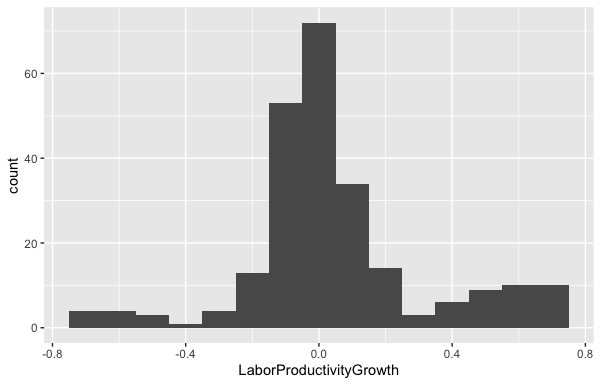
\includegraphics[width=7cm]{chinchilab-template/Pictures/Model3.2_hist_a.png}
    \end{subfigure}
    \begin{subfigure}
    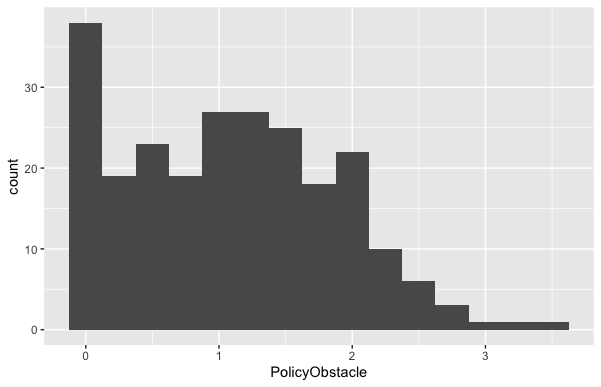
\includegraphics[width=7cm]{chinchilab-template/Pictures/Model3.2_hist_b.png}
    \end{subfigure}
    \begin{subfigure}
    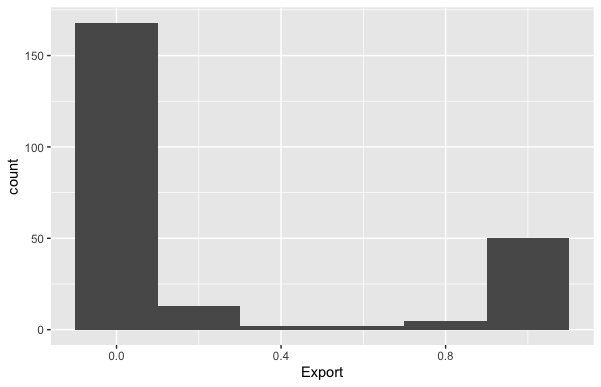
\includegraphics[width=7cm]{chinchilab-template/Pictures/Model3.2_hist_c.png}
    \end{subfigure}
    \begin{subfigure}
    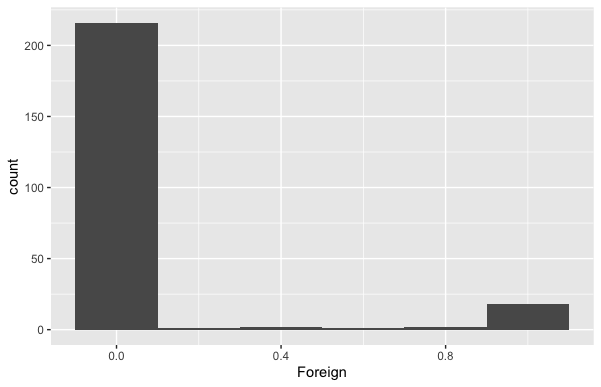
\includegraphics[width=7cm]{chinchilab-template/Pictures/Model3.2_hist_d.png}
    \end{subfigure}
    \caption*{Histogram of Continuous Variables}%
\end{figure}

\begin{figure}[H]
    \centering
    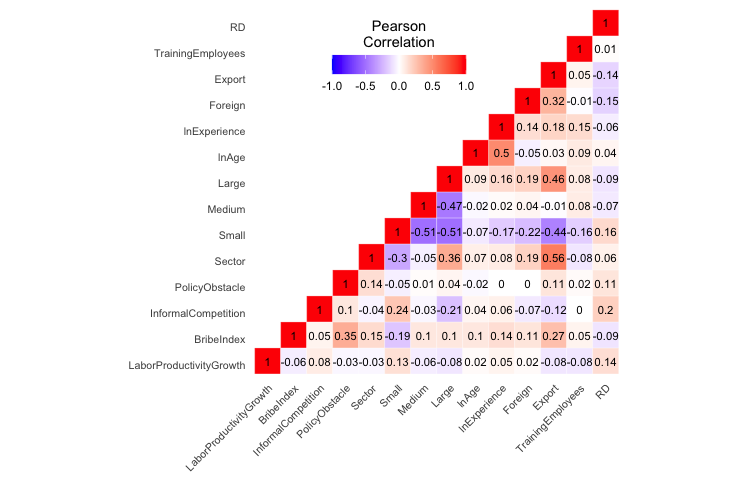
\includegraphics[scale=0.7]{chinchilab-template/Pictures/Model3.2_cor.png}
    \label{fig:my_label}
\end{figure}

\begin{table}[H]
\centering
\scalebox{0.9}{%
\begin{tabular}{lllllll}
\hline
\multicolumn{7}{c}{Variance Inflation Factor (VIF)}                                          \\ \hline
Coefficients                & Baseline & Model 1 & Model 2a & Model 2b & Model 3a & Model 3b \\ \hline
BribeIndex                  &          & 1.10    & 1.23     & 5.86     & 1.11     & 2.24     \\
Policy Obstacle             &          &         & 1.17     & 1.46     &          &          \\
BribeIndex*Policy Obstacle      &          &         &          & 6.91     &          &          \\
Informal Competition        &          &         &          &          & 1.14     & 1.50     \\
BribeIndex*Informal Competition &          &         &          &          &          & 2.59   \\
Sector                      & 1.57     & 1.58    & 1.58     & 1.61     & 1.58     & 1.59     \\
Small                       & 2.03     & 2.03    & 2.04     & 2.05     & 2.14     & 2.14     \\
Medium                      & 1.58     & 1.59    & 1.59     & 1.61     & 1.61     & 1.61     \\
lnAge                       & 1.31     & 1.32    & 1.33     & 1.33     & 1.32     & 1.35     \\
lnExperience                & 1.35     & 1.35    & 1.35     & 1.36     & 1.36     & 1.38     \\
Foreign                     & 1.21     & 1.21    & 1.22     & 1.23     & 1.22     & 1.22     \\
Export                      & 2.05     & 2.11    & 2.12     & 2.20     & 2.12     & 2.13     \\
TrainingEmployees           & 1.09     & 1.09    & 1.09     & 1.09     & 1.09     & 1.09     \\
R\&D                        & 1.12     & 1.12    & 1.14     & 1.14     & 1.15     & 1.16     
\end{tabular}}
\end{table}

\begin{figure}[!t]%
    \centering
    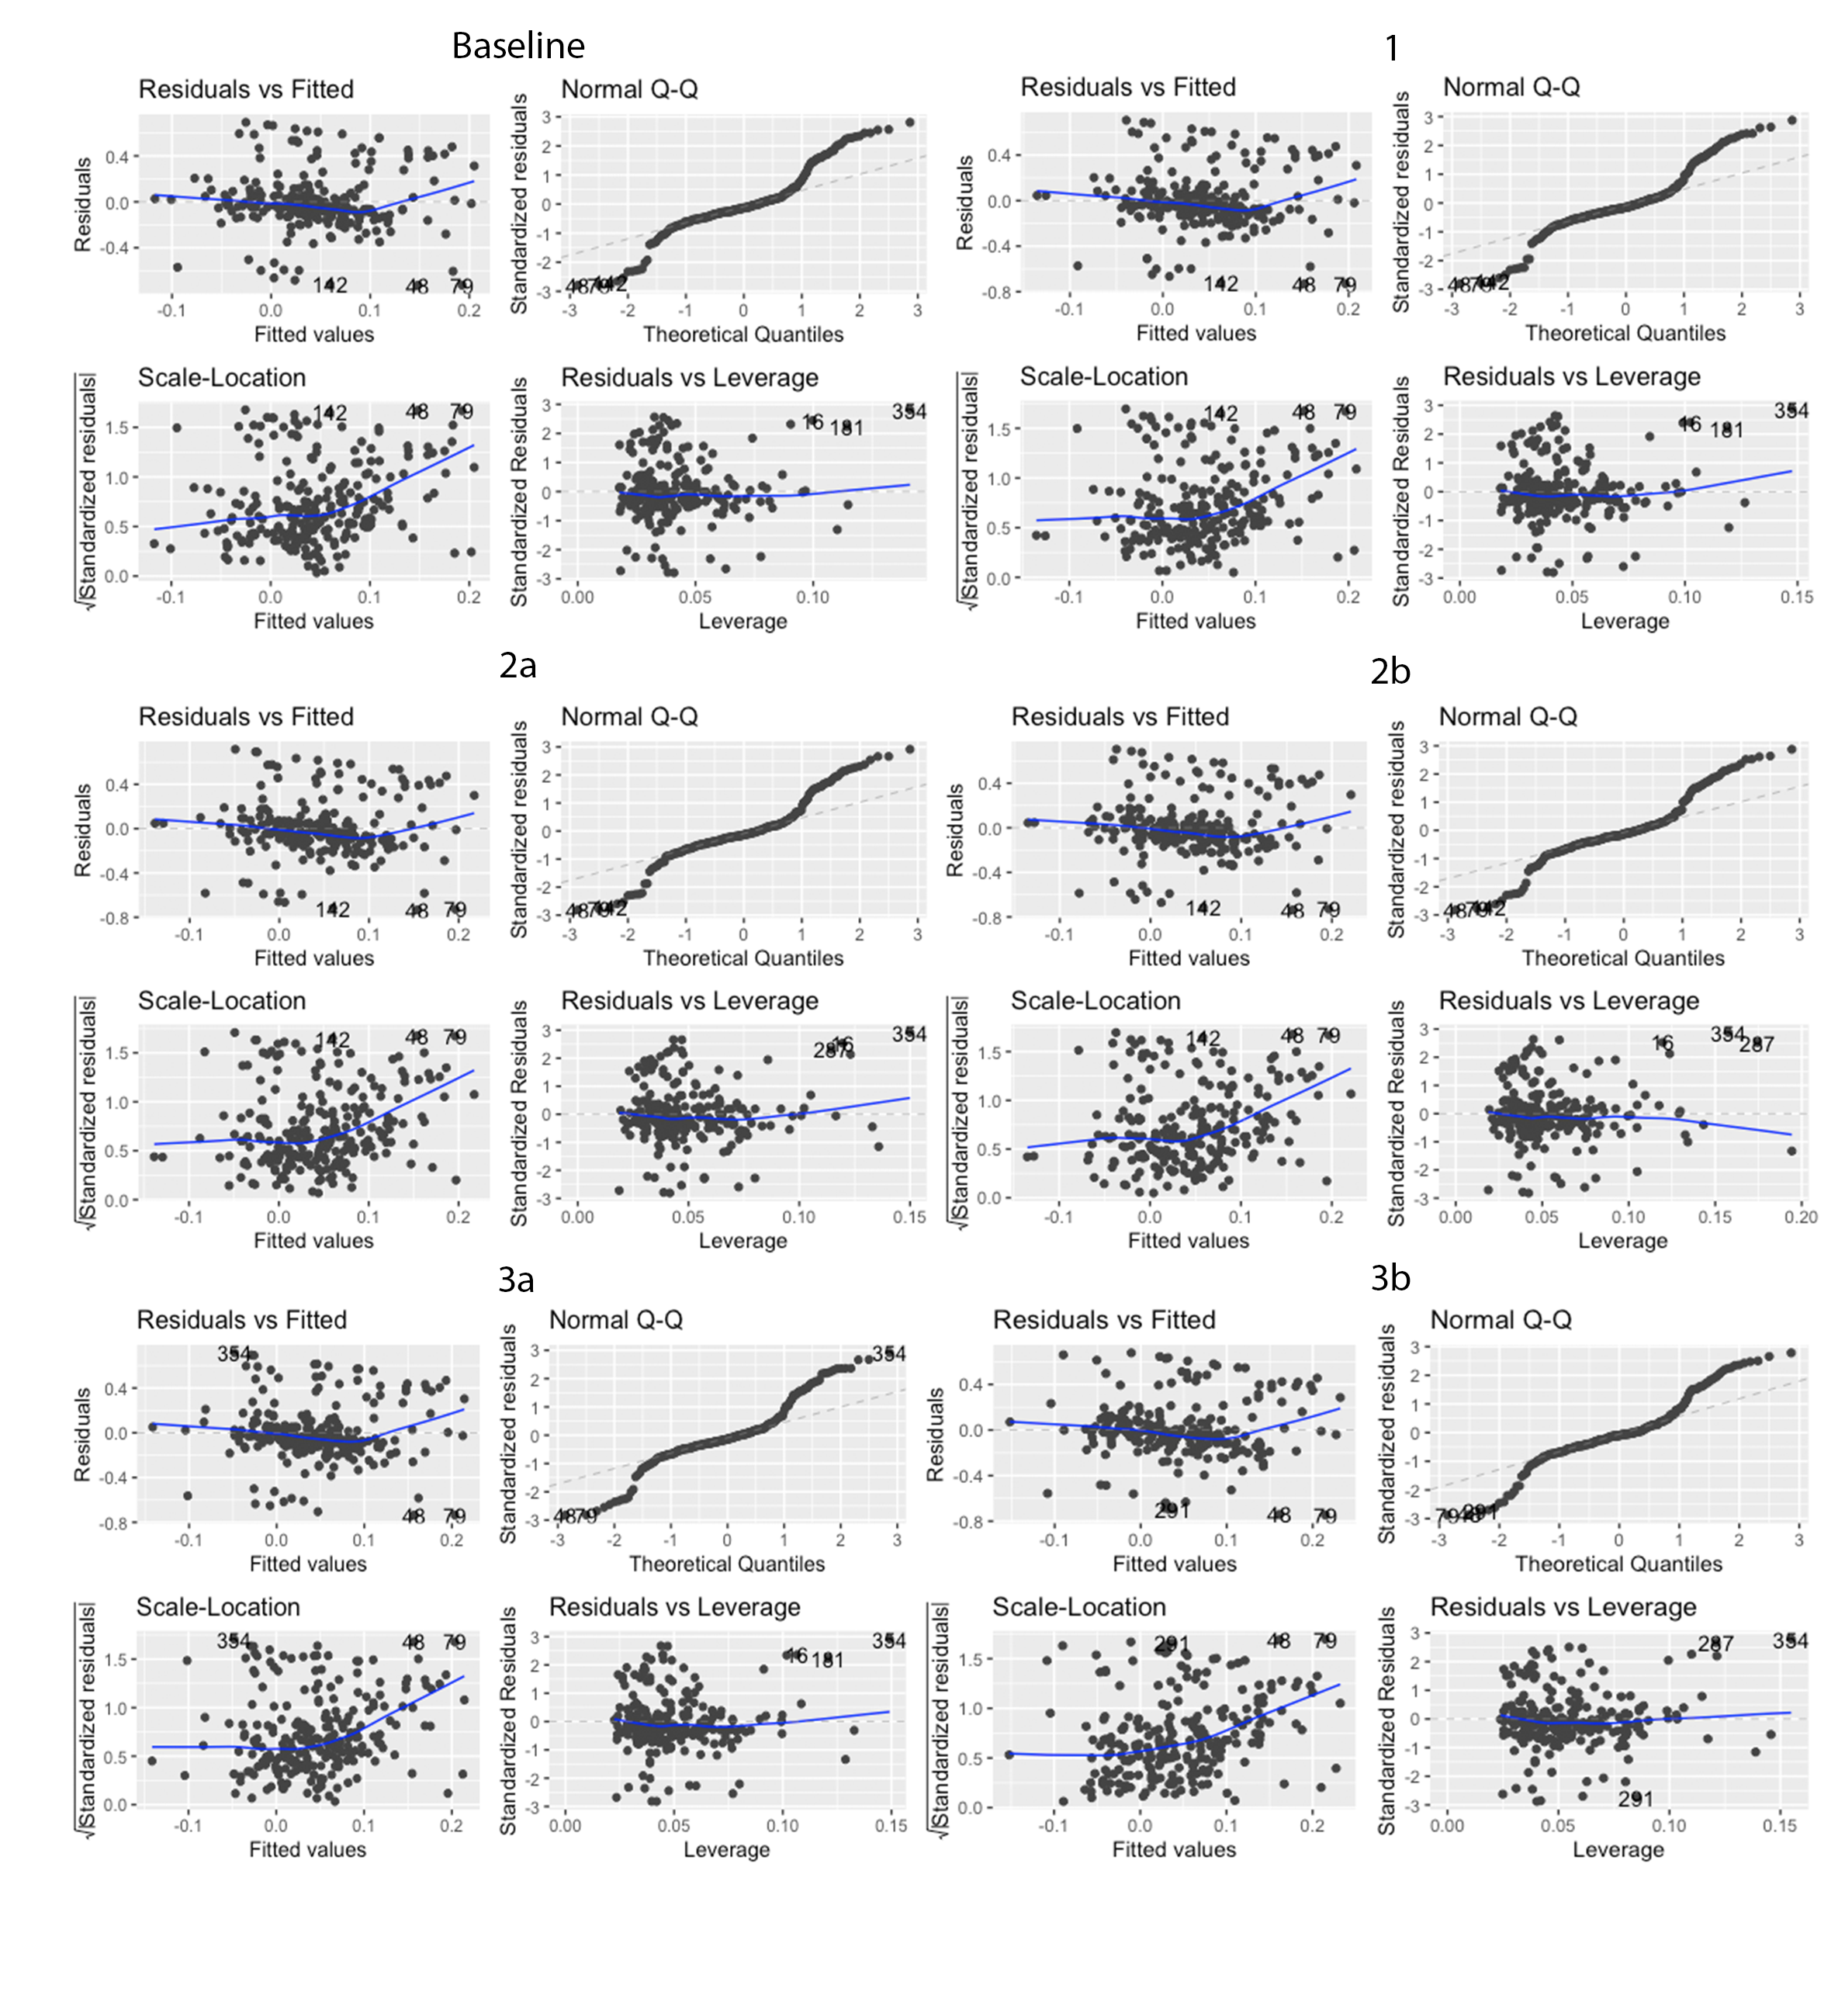
\includegraphics[scale=0.75]{chinchilab-template/Pictures/Model3.2_diag.png}
    \caption*{Diagnostic Plots}%
\end{figure}

\begin{landscape}
\thispagestyle{mylandscape}
\begin{table}[] \centering 
  \caption*{Summary Statistics} 
  \begin{adjustbox}{width=\columnwidth,center}
\begin{tabular}{@{\extracolsep{5pt}}lD{.}{.}{-3} D{.}{.}{-3} D{.}{.}{-3} D{.}{.}{-3} D{.}{.}{-3} D{.}{.}{-3} } 
\\[-1.8ex]\hline 
\hline \\[-1.8ex] 
 & \multicolumn{6}{c}{\textit{Dependent variable:}} \\ 
\cline{2-7} 
\\[-1.8ex] & \multicolumn{6}{c}{LaborProductivityGrowth} \\ 
\\[-1.8ex] & \multicolumn{1}{c}{(1)} & \multicolumn{1}{c}{(2)} & \multicolumn{1}{c}{(3)} & \multicolumn{1}{c}{(4)} & \multicolumn{1}{c}{(5)} & \multicolumn{1}{c}{(6)}\\ 
\hline \\[-1.8ex] 
  BribeIndex &  & -0.027 & -0.016 & -0.060 & -0.031 & 0.048 \\ 
  &  & (0.042) & (0.045) & (0.098) & (0.043) & (0.060) \\ 
  PolicyObstacle &  &  & -0.018 & -0.024 &  &  \\ 
  &  &  & (0.024) & (0.026) &  &  \\ 
  BribeIndex $\times$ PolicyObstacle &  &  &  & 0.031 &  &  \\ 
  &  &  &  & (0.061) &  &  \\ 
  InformalCompetition &  &  &  &  & 0.030 & 0.068 \\ 
  &  &  &  &  & (0.037) & (0.042) \\ 
  BribeIndex $\times$ InformalCompetition &  &  &  &  &  & \cellcolor{yellow}-0.154^{*} \\ 
  &  &  &  &  &  & (0.083) \\ 
 Sector & -0.045 & -0.044 & -0.042 & -0.039 & -0.046 & -0.053 \\ 
  & (0.043) & (0.044) & (0.044) & (0.044) & (0.044) & (0.044) \\ 
  Small & 0.069 & 0.069 & 0.069 & 0.071 & 0.059 & 0.057 \\ 
  & (0.051) & (0.051) & (0.051) & (0.051) & (0.052) & (0.052) \\ 
  Medium & 0.043 & 0.046 & 0.046 & 0.049 & 0.042 & 0.046 \\ 
  & (0.046) & (0.046) & (0.046) & (0.047) & (0.047) & (0.047) \\ 
  lnAge & 0.016 & 0.019 & 0.017 & 0.018 & 0.018 & 0.009 \\ 
  & (0.036) & (0.036) & (0.036) & (0.036) & (0.036) & (0.036) \\ 
  lnExperience & 0.040 & 0.040 & 0.040 & 0.041 & 0.038 & 0.046 \\ 
  & (0.036) & (0.036) & (0.036) & (0.036) & (0.036) & (0.036) \\ 
  Foreign & 0.056 & 0.056 & 0.054 & 0.058 & 0.055 & 0.060 \\ 
  & (0.068) & (0.068) & (0.068) & (0.069) & (0.068) & (0.068) \\ 
  Export & 0.051 & 0.057 & 0.060 & 0.054 & 0.061 & 0.056 \\ 
  & (0.060) & (0.061) & (0.061) & (0.062) & (0.061) & (0.061) \\ 
  TrainingEmployees & -0.055 & -0.055 & -0.054 & -0.053 & -0.055 & -0.053 \\ 
  & (0.036) & (0.036) & (0.036) & (0.036) & (0.036) & (0.036) \\ 
  R\&D & \cellcolor{yellow}0.089^{**} & \cellcolor{yellow}0.088^{**} & \cellcolor{yellow}0.092^{**} & \cellcolor{yellow}0.092^{**} & \cellcolor{yellow}0.082^{*} & \cellcolor{yellow}0.075^{*} \\ 
  & (0.043) & (0.044) & (0.044) & (0.044) & (0.044) & (0.044) \\ 
  Constant & -0.150 & -0.152 & -0.132 & -0.136 & -0.150 & -0.166 \\ 
  & (0.116) & (0.116) & (0.119) & (0.120) & (0.117) & (0.116) \\ 
 \hline \\[-1.8ex] 
Observations & \multicolumn{1}{c}{240} & \multicolumn{1}{c}{240} & \multicolumn{1}{c}{240} & \multicolumn{1}{c}{240} & \multicolumn{1}{c}{240} & \multicolumn{1}{c}{240} \\ 
R$^{2}$ & \multicolumn{1}{c}{0.047} & \multicolumn{1}{c}{0.049} & \multicolumn{1}{c}{0.051} & \multicolumn{1}{c}{0.052} & \multicolumn{1}{c}{0.052} & \multicolumn{1}{c}{0.066} \\ 
Adjusted R$^{2}$ & \multicolumn{1}{c}{0.010} & \multicolumn{1}{c}{0.007} & \multicolumn{1}{c}{0.006} & \multicolumn{1}{c}{0.002} & \multicolumn{1}{c}{0.006} & \multicolumn{1}{c}{0.016} \\ 
Residual Std. Error & \multicolumn{1}{c}{0.266 (df = 230)} & \multicolumn{1}{c}{0.266 (df = 229)} & \multicolumn{1}{c}{0.266 (df = 228)} & \multicolumn{1}{c}{0.267 (df = 227)} & \multicolumn{1}{c}{0.266 (df = 228)} & \multicolumn{1}{c}{0.265 (df = 227)} \\ 
F Statistic & \multicolumn{1}{c}{1.265 (df = 9; 230)} & \multicolumn{1}{c}{1.177 (df = 10; 229)} & \multicolumn{1}{c}{1.120 (df = 11; 228)} & \multicolumn{1}{c}{1.044 (df = 12; 227)} & \multicolumn{1}{c}{1.130 (df = 11; 228)} & \multicolumn{1}{c}{1.334 (df = 12; 227)} \\ 
\hline 
\hline \\[-1.8ex] 
\textit{Note:}  & \multicolumn{6}{r}{$^{*}$p$<$0.1; $^{**}$p$<$0.05; $^{***}$p$<$0.01} \\ 
\end{tabular} 
\end{adjustbox}
\end{table} 
\end{landscape}
%%%%%%%%%%%%%%%%%%%%%%%%%%%%%%%%%%%%%%%%%%%%%%%%%%%%%
%%%%%%%%%%%%%%%%%%%%%%%%%%%%%%%%%%%%%%%%%%%%%%%%%%%
\textbf{\Large Model LIB}
\begin{table}[!htbp] \centering 
  \caption*{}  
\begin{tabular}{@{\extracolsep{5pt}}lccccccc} 
\\[-1.8ex]\hline 
\hline \\[-1.8ex] 
Statistic & \multicolumn{1}{c}{N} & \multicolumn{1}{c}{Mean} & \multicolumn{1}{c}{St. Dev.} & \multicolumn{1}{c}{Min} & \multicolumn{1}{c}{Pctl(25)} & \multicolumn{1}{c}{Pctl(75)} & \multicolumn{1}{c}{Max} \\ 
\hline \\[-1.8ex] 
LaborProductivityGrowth & 223 & 0.049 & 0.270 & $-$0.660 & $-$0.072 & 0.118 & 0.667 \\ 
Inspection.Bribe & 223 & 0.327 & 0.470 & 0 & 0 & 1 & 1 \\ 
InformalCompetition & 223 & 0.475 & 0.501 & 0 & 0 & 1 & 1 \\ 
PolicyObstacle & 223 & 1.089 & 0.786 & 0.000 & 0.500 & 1.750 & 3.500 \\ 
Sector & 223 & 0.430 & 0.496 & 0 & 0 & 1 & 1 \\ 
Small & 223 & 0.363 & 0.482 & 0 & 0 & 1 & 1 \\ 
Medium & 223 & 0.314 & 0.465 & 0 & 0 & 1 & 1 \\ 
Large & 223 & 0.323 & 0.469 & 0 & 0 & 1 & 1 \\ 
lnAge & 223 & 2.674 & 0.547 & 1.386 & 2.398 & 3.135 & 4.454 \\ 
lnExperience & 223 & 2.944 & 0.542 & 0.693 & 2.708 & 3.258 & 3.807 \\ 
Foreign & 223 & 0.078 & 0.265 & 0 & 0 & 0 & 1 \\ 
Export & 223 & 0.249 & 0.408 & 0 & 0 & 0.3 & 1 \\ 
TrainingEmployees & 223 & 0.453 & 0.499 & 0 & 0 & 1 & 1 \\ 
R\&D & 223 & 0.242 & 0.429 & 0 & 0 & 0 & 1 \\ 
\hline \\[-1.8ex] 
\end{tabular} 
\end{table} 

\begin{figure}[H]%
    \centering
    \begin{subfigure}
    \includegraphics[width=7cm]{chinchilab-template/Pictures/Model3.3_hist_a.png}
    \end{subfigure}
    \begin{subfigure}
    \includegraphics[width=7cm]{chinchilab-template/Pictures/Model3.3_hist_b.png}
    \end{subfigure}
    \begin{subfigure}
    \includegraphics[width=7cm]{chinchilab-template/Pictures/Model3.3_hist_c.png}
    \end{subfigure}
    \begin{subfigure}
    \includegraphics[width=7cm]{chinchilab-template/Pictures/Model3.3_hist_d.png}
    \end{subfigure}
    \caption*{Histogram of Continuous Variables}%
\end{figure}

\begin{figure}[H]
    \centering
    \includegraphics[scale=0.6]{chinchilab-template/Pictures/Model3.3_cor.png}
    \label{fig:my_label}
\end{figure}

\begin{table}[H]
\centering
\scalebox{0.9}{%
\begin{tabular}{lllllll}
\hline
\multicolumn{7}{c}{Variance Inflation Factor (VIF)}                                          \\ \hline
Coefficients                & Baseline & Model 1 & Model 2a & Model 2b & Model 3a & Model 3b \\ \hline
Inspection.Bribe                  &          & 1.08    & 1.14     & 3.92     & 1.11     & 2.17     \\
Policy Obstacle             &          &         & 1.11     & 1.62     &          &          \\
Inspection.Bribe*Policy Obstacle      &          &         &          & 4.96     &          &          \\
Informal Competition        &          &         &          &          & 1.16     & 1.74     \\
Inspection.Bribe*Informal Competition &          &         &          &          &          & 2.95 \\
Sector                      & 1.61     & 1.63    & 1.64     & 1.66     & 1.64     & 1.64     \\
Small                       & 2.07     & 2.07    & 2.07     & 2.07     & 2.15     & 2.16     \\
Medium                      & 1.62     & 1.63    & 1.63     & 1.64     & 1.64     & 1.64     \\
lnAge                       & 1.30     & 1.31    & 1.31     & 1.32     & 1.31     & 1.32     \\
lnExperience                & 1.34     & 1.35    & 1.35     & 1.35     & 1.36     & 1.36     \\
Foreign                     & 1.22     & 1.24    & 1.24     & 1.24     & 1.24     & 1.24     \\
Export                      & 2.11     & 2.11    & 2.12     & 2.16     & 2.11     & 2.11     \\
TrainingEmployees           & 1.09     & 1.09    & 1.09     & 1.12     & 1.09     & 1.14     \\
R\&D                        & 1.13     & 1.17    & 1.20     & 1.20     & 1.21     & 1.25     
\end{tabular}}
\end{table}

\begin{figure}[!t]%
    \centering
    \includegraphics[scale=0.75]{chinchilab-template/Pictures/Model3.3_diag.png}
    \caption*{Diagnostic Plots}%
\end{figure}

\begin{landscape}
\thispagestyle{mylandscape}
\begin{table}[] \centering 
  \caption*{Summary Statistics} 
  \begin{adjustbox}{width=\columnwidth,center}
\begin{tabular}{@{\extracolsep{5pt}}lD{.}{.}{-3} D{.}{.}{-3} D{.}{.}{-3} D{.}{.}{-3} D{.}{.}{-3} D{.}{.}{-3} } 
\\[-1.8ex]\hline 
\hline \\[-1.8ex] 
 & \multicolumn{6}{c}{\textit{Dependent variable:}} \\ 
\cline{2-7} 
\\[-1.8ex] & \multicolumn{6}{c}{LaborProductivityGrowth} \\ 
\\[-1.8ex] & \multicolumn{1}{c}{(1)} & \multicolumn{1}{c}{(2)} & \multicolumn{1}{c}{(3)} & \multicolumn{1}{c}{(4)} & \multicolumn{1}{c}{(5)} & \multicolumn{1}{c}{(6)}\\ 
\hline \\[-1.8ex] 
  Inspection.Bribe &  & -0.024 & -0.016 & -0.031 & -0.029 & 0.009 \\ 
  &  & (0.040) & (0.041) & (0.076) & (0.040) & (0.057) \\ 
  PolicyObstacle &  &  & -0.019 & -0.023 &  &  \\ 
  &  &  & (0.024) & (0.029) &  &  \\ 
  Inspection.Bribe $\times$ PolicyObstacle &  &  &  & 0.012 &  &  \\ 
  &  &  &  & (0.053) &  &  \\ 
  InformalCompetition &  &  &  &  & 0.035 & 0.061 \\ 
  &  &  &  &  & (0.039) & (0.048) \\ 
  Inspection.Bribe $\times$ InformalCompetition &  &  &  &  &  & -0.077 \\ 
  &  &  &  &  &  & (0.081) \\ 
 Sector & -0.047 & -0.044 & -0.042 & -0.041 & -0.047 & -0.047 \\ 
  & (0.046) & (0.047) & (0.047) & (0.047) & (0.047) & (0.047) \\ 
  Small & 0.058 & 0.058 & 0.057 & 0.057 & 0.048 & 0.051 \\ 
  & (0.054) & (0.054) & (0.054) & (0.054) & (0.055) & (0.055) \\ 
  Medium & 0.026 & 0.028 & 0.028 & 0.027 & 0.025 & 0.026 \\ 
  & (0.049) & (0.050) & (0.050) & (0.050) & (0.050) & (0.050) \\ 
  lnAge & 0.012 & 0.011 & 0.010 & 0.010 & 0.010 & 0.007 \\ 
  & (0.038) & (0.038) & (0.038) & (0.038) & (0.038) & (0.038) \\ 
  lnExperience & 0.036 & 0.038 & 0.037 & 0.038 & 0.035 & 0.037 \\ 
  & (0.039) & (0.039) & (0.039) & (0.039) & (0.039) & (0.039) \\ 
  Foreign & 0.091 & 0.086 & 0.084 & 0.085 & 0.087 & 0.086 \\ 
  & (0.075) & (0.076) & (0.076) & (0.076) & (0.076) & (0.076) \\ 
  Export & 0.035 & 0.035 & 0.039 & 0.037 & 0.038 & 0.039 \\ 
  & (0.064) & (0.064) & (0.065) & (0.065) & (0.064) & (0.064) \\ 
  TrainingEmployees & -0.058 & -0.057 & -0.056 & -0.055 & -0.058 & -0.051 \\ 
  & (0.038) & (0.038) & (0.038) & (0.038) & (0.038) & (0.039) \\ 
  R\&D & \cellcolor{yellow}0.083^{*} & \cellcolor{yellow}0.078^{*} & \cellcolor{yellow}0.084^{*} & \cellcolor{yellow}0.084^{*} & 0.070 & 0.063 \\ 
  & (0.045) & (0.046) & (0.046) & (0.046) & (0.046) & (0.047) \\ 
  Constant & -0.110 & -0.103 & -0.084 & -0.081 & -0.099 & -0.113 \\ 
  & (0.125) & (0.126) & (0.128) & (0.129) & (0.126) & (0.127) \\ 
 \hline \\[-1.8ex] 
Observations & \multicolumn{1}{c}{223} & \multicolumn{1}{c}{223} & \multicolumn{1}{c}{223} & \multicolumn{1}{c}{223} & \multicolumn{1}{c}{223} & \multicolumn{1}{c}{223} \\ 
R$^{2}$ & \multicolumn{1}{c}{0.046} & \multicolumn{1}{c}{0.047} & \multicolumn{1}{c}{0.050} & \multicolumn{1}{c}{0.050} & \multicolumn{1}{c}{0.051} & \multicolumn{1}{c}{0.055} \\ 
Adjusted R$^{2}$ & \multicolumn{1}{c}{0.005} & \multicolumn{1}{c}{0.002} & \multicolumn{1}{c}{0.0005} & \multicolumn{1}{c}{-0.004} & \multicolumn{1}{c}{0.001} & \multicolumn{1}{c}{0.001} \\ 
Residual Std. Error & \multicolumn{1}{c}{0.269 (df = 213)} & \multicolumn{1}{c}{0.269 (df = 212)} & \multicolumn{1}{c}{0.270 (df = 211)} & \multicolumn{1}{c}{0.270 (df = 210)} & \multicolumn{1}{c}{0.269 (df = 211)} & \multicolumn{1}{c}{0.269 (df = 210)} \\ 
F Statistic & \multicolumn{1}{c}{1.130 (df = 9; 213)} & \multicolumn{1}{c}{1.049 (df = 10; 212)} & \multicolumn{1}{c}{1.010 (df = 11; 211)} & \multicolumn{1}{c}{0.926 (df = 12; 210)} & \multicolumn{1}{c}{1.025 (df = 11; 211)} & \multicolumn{1}{c}{1.015 (df = 12; 210)} \\ 
\hline 
\hline \\[-1.8ex] 
\textit{Note:}  & \multicolumn{6}{r}{$^{*}$p$<$0.1; $^{**}$p$<$0.05; $^{***}$p$<$0.01} \\ 
\end{tabular} 
\end{adjustbox}
\end{table} 
\end{landscape}

\textbf{\Large Model IB}
\begin{table}[H] \centering 
  \caption*{} 
\begin{tabular}{@{\extracolsep{5pt}}lccccccc} 
\\[-1.8ex]\hline 
\hline \\[-1.8ex] 
Statistic & \multicolumn{1}{c}{N} & \multicolumn{1}{c}{Mean} & \multicolumn{1}{c}{St. Dev.} & \multicolumn{1}{c}{Min} & \multicolumn{1}{c}{Pctl(25)} & \multicolumn{1}{c}{Pctl(75)} & \multicolumn{1}{c}{Max} \\ 
\hline \\[-1.8ex] 
InnovationIndex & 185 & 0.476 & 0.501 & 0 & 0 & 1 & 1 \\ 
Bribes & 185 & 0.027 & 0.051 & 0.000 & 0.000 & 0.030 & 0.200 \\ 
InformalCompetition & 185 & 0.535 & 0.500 & 0 & 0 & 1 & 1 \\ 
PolicyObstacle & 185 & 1.003 & 0.738 & 0 & 0.2 & 1.5 & 4 \\ 
Sector & 185 & 0.427 & 0.496 & 0 & 0 & 1 & 1 \\ 
Small & 185 & 0.400 & 0.491 & 0 & 0 & 1 & 1 \\ 
Medium & 185 & 0.281 & 0.451 & 0 & 0 & 1 & 1 \\ 
Large & 185 & 0.319 & 0.467 & 0 & 0 & 1 & 1 \\ 
lnAge & 185 & 2.437 & 0.747 & 0.693 & 1.946 & 3.045 & 3.367 \\ 
lnExperience & 185 & 2.833 & 0.668 & 0.000 & 2.485 & 3.258 & 3.807 \\ 
Foreign & 185 & 0.095 & 0.285 & 0 & 0 & 0 & 1 \\ 
Export & 185 & 0.260 & 0.410 & 0 & 0 & 0.3 & 1 \\ 
TrainingEmployees & 185 & 0.357 & 0.480 & 0 & 0 & 1 & 1 \\ 
R\&D & 185 & 0.238 & 0.427 & 0 & 0 & 0 & 1 \\ 
QualityCertificate & 185 & 0.286 & 0.453 & 0 & 0 & 1 & 1 \\ 
\hline \\[-1.8ex] 
\end{tabular}
\end{table} 

\begin{figure}[H]%
    \centering
    \begin{subfigure}
    \includegraphics[width=7cm]{chinchilab-template/Pictures/Model4_hist_a.png}
    \end{subfigure}
    \begin{subfigure}
    \includegraphics[width=7cm]{chinchilab-template/Pictures/Model4_hist_b.png}
    \end{subfigure}
    \begin{subfigure}
    \includegraphics[width=7cm]{chinchilab-template/Pictures/Model4_hist_c.png}
    \end{subfigure}
    \begin{subfigure}
    \includegraphics[width=7cm]{chinchilab-template/Pictures/Model4_hist_d.png}
    \end{subfigure}
    \begin{subfigure}
    \includegraphics[width=7cm]{chinchilab-template/Pictures/Model4_hist_e.png}
    \end{subfigure}
    \caption*{Histogram of Dependent and Continuous Variables}%
\end{figure}
\clearpage
\newpage
%%%%%%%%%%%%%%%%%%%%%%%%%%%%%%%%%%%%%%%%%%%%%%%%%
\textbf{\Large Model IBI}
\begin{table}[H] \centering 
  \caption*{} 
\begin{tabular}{@{\extracolsep{5pt}}lccccccc} 
\\[-1.8ex]\hline 
\hline \\[-1.8ex] 
Statistic & \multicolumn{1}{c}{N} & \multicolumn{1}{c}{Mean} & \multicolumn{1}{c}{St. Dev.} & \multicolumn{1}{c}{Min} & \multicolumn{1}{c}{Pctl(25)} & \multicolumn{1}{c}{Pctl(75)} & \multicolumn{1}{c}{Max} \\ 
\hline \\[-1.8ex] 
InnovationIndex & 289 & 0.540 & 0.499 & 0 & 0 & 1 & 1 \\ 
BribeIndex & 289 & 0.211 & 0.409 & 0 & 0 & 0 & 1 \\ 
InformalCompetition & 289 & 0.488 & 0.501 & 0 & 0 & 1 & 1 \\ 
PolicyObstacle & 289 & 1.089 & 0.785 & 0.000 & 0.500 & 1.750 & 3.500 \\ 
Sector & 289 & 0.419 & 0.494 & 0 & 0 & 1 & 1 \\ 
Small & 289 & 0.398 & 0.490 & 0 & 0 & 1 & 1 \\ 
Medium & 289 & 0.301 & 0.460 & 0 & 0 & 1 & 1 \\ 
Large & 289 & 0.301 & 0.460 & 0 & 0 & 1 & 1 \\ 
lnAge & 289 & 2.486 & 0.740 & 0.693 & 2.079 & 3.091 & 4.454 \\ 
lnExperience & 289 & 2.830 & 0.689 & 0.000 & 2.485 & 3.258 & 3.807 \\ 
Foreign & 289 & 0.091 & 0.282 & 0 & 0 & 0 & 1 \\ 
Export & 289 & 0.249 & 0.406 & 0 & 0 & 0.3 & 1 \\ 
TrainingEmployees & 289 & 0.429 & 0.496 & 0 & 0 & 1 & 1 \\ 
R\&D & 289 & 0.225 & 0.418 & 0 & 0 & 0 & 1 \\ 
QualityCertificate & 289 & 0.270 & 0.445 & 0 & 0 & 1 & 1 \\ 
\hline \\[-1.8ex] 
\end{tabular} 
\end{table} 

\begin{figure}[H]%
    \centering
    \begin{subfigure}
    \includegraphics[width=7cm]{chinchilab-template/Pictures/Model4.2_hist_a.png}
    \end{subfigure}
    \begin{subfigure}
    \includegraphics[width=7cm]{chinchilab-template/Pictures/Model4.2_hist_b.png}
    \end{subfigure}
    \begin{subfigure}
    \includegraphics[width=7cm]{chinchilab-template/Pictures/Model4.2_hist_c.png}
    \end{subfigure}
    \begin{subfigure}
    \includegraphics[width=7cm]{chinchilab-template/Pictures/Model4.2_hist_d.png}
    \end{subfigure}
    \caption*{Histogram of Dependent and Continuous Variables}%
\end{figure}
\clearpage
\newpage
%%%%%%%%%%%%%%%%%%%%%%%%%%%%%%%%%%%%%%%%%%%%%%%%%
\textbf{\Large Model IIB}
\begin{table}[H] \centering 
  \caption*{Summary Statistics} 
\begin{tabular}{@{\extracolsep{5pt}}lccccccc} 
\\[-1.8ex]\hline 
\hline \\[-1.8ex] 
Statistic & \multicolumn{1}{c}{N} & \multicolumn{1}{c}{Mean} & \multicolumn{1}{c}{St. Dev.} & \multicolumn{1}{c}{Min} & \multicolumn{1}{c}{Pctl(25)} & \multicolumn{1}{c}{Pctl(75)} & \multicolumn{1}{c}{Max} \\ 
\hline \\[-1.8ex] 
InnovationIndex & 268 & 0.541 & 0.499 & 0 & 0 & 1 & 1 \\ 
Inspection.Bribe & 268 & 0.317 & 0.466 & 0 & 0 & 1 & 1 \\ 
InformalCompetition & 268 & 0.485 & 0.501 & 0 & 0 & 1 & 1 \\ 
PolicyObstacle & 268 & 1.096 & 0.788 & 0.000 & 0.500 & 1.750 & 3.500 \\ 
Sector & 268 & 0.422 & 0.495 & 0 & 0 & 1 & 1 \\ 
Small & 268 & 0.396 & 0.490 & 0 & 0 & 1 & 1 \\ 
Medium & 268 & 0.299 & 0.458 & 0 & 0 & 1 & 1 \\ 
Large & 268 & 0.306 & 0.462 & 0 & 0 & 1 & 1 \\ 
lnAge & 268 & 2.484 & 0.741 & 0.693 & 2.079 & 3.091 & 4.454 \\ 
lnExperience & 268 & 2.838 & 0.680 & 0.000 & 2.545 & 3.258 & 3.807 \\ 
Foreign & 268 & 0.080 & 0.268 & 0 & 0 & 0 & 1 \\ 
Export & 268 & 0.247 & 0.406 & 0 & 0 & 0.3 & 1 \\ 
TrainingEmployees & 268 & 0.448 & 0.498 & 0 & 0 & 1 & 1 \\ 
R\&D & 268 & 0.243 & 0.429 & 0 & 0 & 0 & 1 \\ 
QualityCertificate & 268 & 0.265 & 0.442 & 0 & 0 & 1 & 1 \\ 
\hline \\[-1.8ex] 
\end{tabular} 
\end{table} 

\begin{figure}[H]%
    \centering
    \begin{subfigure}
    \includegraphics[width=7cm]{chinchilab-template/Pictures/Model4.3_hist_a.png}
    \end{subfigure}
    \begin{subfigure}
    \includegraphics[width=7cm]{chinchilab-template/Pictures/Model4.3_hist_b.png}
    \end{subfigure}
    \begin{subfigure}
    \includegraphics[width=7cm]{chinchilab-template/Pictures/Model4.3_hist_c.png}
    \end{subfigure}
    \begin{subfigure}
    \includegraphics[width=7cm]{chinchilab-template/Pictures/Model4.3_hist_d.png}
    \end{subfigure}
    \caption*{Histogram of Dependent and Continuous Variables}%
\end{figure}
